\documentclass[a4paper]{book}
\usepackage{a4wide}
\usepackage{makeidx}
\usepackage{fancyhdr}
\usepackage{graphicx}
\usepackage{multicol}
\usepackage{float}
\usepackage{textcomp}
\usepackage{alltt}
\usepackage{times}
\usepackage{ifpdf}
\ifpdf
\usepackage[pdftex,
            pagebackref=true,
            colorlinks=true,
            linkcolor=blue,
            unicode
           ]{hyperref}
\else
\usepackage[ps2pdf,
            pagebackref=true,
            colorlinks=true,
            linkcolor=blue,
            unicode
           ]{hyperref}
\usepackage{pspicture}
\fi
\usepackage[utf8]{inputenc}
\usepackage{doxygen}
\makeindex
\setcounter{tocdepth}{3}
\renewcommand{\footrulewidth}{0.4pt}
\begin{document}
\begin{titlepage}
\vspace*{7cm}
\begin{center}
{\Large Reference Manual}\\
\vspace*{1cm}
{\large Generated by Doxygen 1.5.6}\\
\vspace*{0.5cm}
{\small Tue Sep 20 18:46:12 2011}\\
\end{center}
\end{titlepage}
\clearemptydoublepage
\pagenumbering{roman}
\tableofcontents
\clearemptydoublepage
\pagenumbering{arabic}
\chapter{GenomicTools}
\label{index}\hypertarget{index}{}\hypertarget{index_intro}{}\section{Introduction}\label{index_intro}
{\bf GenomicTools} is a flexible computational platform for the analysis and manipulation of high-throughput sequencing data such as DNA-seq, RNA-seq, ChIP-seq and MethylC-seq. GenomicTools implements a variety of mathematical operations between sets of genomic regions thereby enabling the prototyping of computational pipelines that can address a wide spectrum of tasks from preprocessing and quality control to meta-analyses. For example, the user can easily create average read profiles across transcriptional start sites or enhancer sites, quickly prototype customized peak discovery methods for ChIP-seq experiments, perform genome-wide statistical tests such as enrichment analyses, design controls via appropriate randomization schemes, among other applications. In addition to enabling rapid prototyping, the GenomicTools platform is designed to analyze large-datasets of any size by minimizing memory requirements. Compared to Bioconductor packages, it offers a $\sim$10-fold improvement by relying on single-pass processing and fast I/O implementation. When analyzing hundreds of patient datasets, this is a significant advantage. Finally, the GenomicTools platform supports the widely used BED format to facilitate visualization as well as integration with existing platforms and pipelines such as Galaxy or Bioconductor.\hypertarget{index_download}{}\section{Download and install}\label{index_download}
{\bf GenomicTools} can be downloaded from \href{http://http://code.google.com/p/ibm-cbc-genomic-tools/}{\tt code.google.com}. To install it, simply enter the src subdirectory and type make. This will create the executables in the bin subdirectory (which you may choose to included in your path). 
\chapter{Class Index}
\section{Class Hierarchy}
This inheritance list is sorted roughly, but not completely, alphabetically:\begin{CompactList}
\item \contentsline{section}{Chromosomes}{\pageref{classChromosomes}}{}
\item \contentsline{section}{FileBuffer}{\pageref{classFileBuffer}}{}
\item \contentsline{section}{GenomicInterval}{\pageref{classGenomicInterval}}{}
\item \contentsline{section}{GenomicIntervalSetAsArray}{\pageref{classGenomicIntervalSetAsArray}}{}
\item \contentsline{section}{GenomicRegion}{\pageref{classGenomicRegion}}{}
\begin{CompactList}
\item \contentsline{section}{GenomicRegionBED}{\pageref{classGenomicRegionBED}}{}
\item \contentsline{section}{GenomicRegionBEDToREG}{\pageref{classGenomicRegionBEDToREG}}{}
\item \contentsline{section}{GenomicRegionGFF}{\pageref{classGenomicRegionGFF}}{}
\item \contentsline{section}{GenomicRegionGFFToREG}{\pageref{classGenomicRegionGFFToREG}}{}
\item \contentsline{section}{GenomicRegionSAM}{\pageref{classGenomicRegionSAM}}{}
\item \contentsline{section}{GenomicRegionSAMToREG}{\pageref{classGenomicRegionSAMToREG}}{}
\end{CompactList}
\item \contentsline{section}{GenomicRegionSet}{\pageref{classGenomicRegionSet}}{}
\begin{CompactList}
\item \contentsline{section}{IndexedGenomicRegionSet}{\pageref{classIndexedGenomicRegionSet}}{}
\end{CompactList}
\item \contentsline{section}{GenomicRegionSetOverlapScanner}{\pageref{classGenomicRegionSetOverlapScanner}}{}
\item \contentsline{section}{GenomicRegionSetScanner}{\pageref{classGenomicRegionSetScanner}}{}
\item \contentsline{section}{Progress}{\pageref{classProgress}}{}
\end{CompactList}

\chapter{Class Index}
\section{Class List}
Here are the classes, structs, unions and interfaces with brief descriptions:\begin{DoxyCompactList}
\item\contentsline{section}{\hyperlink{classChromosomes}{Chromosomes} (This class is used to store chromosome DNA sequences )}{\pageref{classChromosomes}}{}
\item\contentsline{section}{\hyperlink{classFileBuffer}{FileBuffer} (Abstract class for reading lines from file )}{\pageref{classFileBuffer}}{}
\item\contentsline{section}{\hyperlink{classFileBufferBAM}{FileBufferBAM} (Class for reading lines from file in BAM format )}{\pageref{classFileBufferBAM}}{}
\item\contentsline{section}{\hyperlink{classFileBufferGZ}{FileBufferGZ} (Class for reading lines from file in GZ format )}{\pageref{classFileBufferGZ}}{}
\item\contentsline{section}{\hyperlink{classFileBufferText}{FileBufferText} (Class for reading lines from text file or standard input )}{\pageref{classFileBufferText}}{}
\item\contentsline{section}{\hyperlink{classGenomicInterval}{GenomicInterval} (Set of CIGAR operations that map to the fragment sequence (SAM format) )}{\pageref{classGenomicInterval}}{}
\item\contentsline{section}{\hyperlink{classGenomicIntervalSetAsArray}{GenomicIntervalSetAsArray} (\mbox{[}UNDER DEVELOPMENT\mbox{]} This class implements an array of genomic intervals )}{\pageref{classGenomicIntervalSetAsArray}}{}
\item\contentsline{section}{\hyperlink{classGenomicRegion}{GenomicRegion} (This class implements the genomic regions (i.e. ordered sets of genomic intervals) )}{\pageref{classGenomicRegion}}{}
\item\contentsline{section}{\hyperlink{classGenomicRegionBED}{GenomicRegionBED} (This class processes genomic regions in BED format )}{\pageref{classGenomicRegionBED}}{}
\item\contentsline{section}{\hyperlink{classGenomicRegionBEDToREG}{GenomicRegionBEDToREG} (This class reads BED files but converts them internally to the REG format, so all operations are performed on the REG format )}{\pageref{classGenomicRegionBEDToREG}}{}
\item\contentsline{section}{\hyperlink{classGenomicRegionGFF}{GenomicRegionGFF} (This class processes genomic regions in SAM format )}{\pageref{classGenomicRegionGFF}}{}
\item\contentsline{section}{\hyperlink{classGenomicRegionGFFToREG}{GenomicRegionGFFToREG} (This class reads GFF files but converts them internally to the REG format, so all operations are performed on the REG format )}{\pageref{classGenomicRegionGFFToREG}}{}
\item\contentsline{section}{\hyperlink{classGenomicRegionSAM}{GenomicRegionSAM} (This class processes genomic regions in SAM format )}{\pageref{classGenomicRegionSAM}}{}
\item\contentsline{section}{\hyperlink{classGenomicRegionSAMToREG}{GenomicRegionSAMToREG} (This class reads SAM files but converts them internally to the REG format, so all operations are performed on the REG format )}{\pageref{classGenomicRegionSAMToREG}}{}
\item\contentsline{section}{\hyperlink{classGenomicRegionSEQ}{GenomicRegionSEQ} (This class implements the genomic regions REG format with attached sequence )}{\pageref{classGenomicRegionSEQ}}{}
\item\contentsline{section}{\hyperlink{classGenomicRegionSet}{GenomicRegionSet} (This class is used to read and manipulate a set of genomic regions from a file or from standard input )}{\pageref{classGenomicRegionSet}}{}
\item\contentsline{section}{\hyperlink{classGenomicRegionSetOverlaps}{GenomicRegionSetOverlaps} (Abstract class for computing overlaps between genomic regions )}{\pageref{classGenomicRegionSetOverlaps}}{}
\item\contentsline{section}{\hyperlink{classGenomicRegionSetScanner}{GenomicRegionSetScanner} (This class is used to scan a set of regions by sliding windows. See detailed description below for an example )}{\pageref{classGenomicRegionSetScanner}}{}
\item\contentsline{section}{\hyperlink{classProgress}{Progress} (This class is used to report progress of loop computations )}{\pageref{classProgress}}{}
\item\contentsline{section}{\hyperlink{classSortedGenomicRegionSetOverlaps}{SortedGenomicRegionSetOverlaps} (This class is used to find overlaps between two genomic regions sets. See detailed description below for an example )}{\pageref{classSortedGenomicRegionSetOverlaps}}{}
\item\contentsline{section}{\hyperlink{classUnsortedGenomicRegionSetOverlaps}{UnsortedGenomicRegionSetOverlaps} (Class for computing overlaps between unsorted regions )}{\pageref{classUnsortedGenomicRegionSetOverlaps}}{}
\end{DoxyCompactList}

\chapter{Class Documentation}
\hypertarget{classChromosomes}{
\section{Chromosomes Class Reference}
\label{classChromosomes}\index{Chromosomes@{Chromosomes}}
}
This class is used to store chromosome DNA sequences.  


{\tt \#include $<$genomic\_\-intervals.h$>$}

\subsection*{Public Types}
\begin{CompactItemize}
\item 
\hypertarget{classChromosomes_4a233d2b7fabc1a589cbbafd5d0ea243}{
typedef \hyperlink{classChromosomes_8e40e7c99c6c0a40713c7785ba5b5ac4}{map}$<$ string, pair$<$ char $\ast$, size\_\-t $>$ $>$ \hyperlink{classChromosomes_4a233d2b7fabc1a589cbbafd5d0ea243}{ChromosomeSeqData}}
\label{classChromosomes_4a233d2b7fabc1a589cbbafd5d0ea243}

\begin{CompactList}\small\item\em for every chromosome, store a pointer to its sequence, and its size. \item\end{CompactList}\end{CompactItemize}
\subsection*{Public Member Functions}
\begin{CompactItemize}
\item 
\hyperlink{classChromosomes_a596430d4a05ce0dc4d4f43c650db83e}{Chromosomes} (char $\ast$\hyperlink{classChromosomes_8df459fcb5ad98a2524fd51ac2b5a60c}{map\_\-dir}, char $\ast$\hyperlink{classChromosomes_9c690f19e04e80b056dac2072476f24c}{map\_\-name})
\begin{CompactList}\small\item\em Class constructor. \item\end{CompactList}\item 
\hyperlink{classChromosomes_bb3466c6c94f42f22a872b043c415b67}{Chromosomes} (char $\ast$fasta\_\-file, bool \hyperlink{classChromosomes_954bae240564f6f589a30d253291eb75}{verbose})
\begin{CompactList}\small\item\em Class constructor. \item\end{CompactList}\item 
\hypertarget{classChromosomes_0b04a0781b2ff7088dd8046493385003}{
\hyperlink{classChromosomes_0b04a0781b2ff7088dd8046493385003}{$\sim$Chromosomes} ()}
\label{classChromosomes_0b04a0781b2ff7088dd8046493385003}

\begin{CompactList}\small\item\em Class destructor. \item\end{CompactList}\item 
\hypertarget{classChromosomes_2378b5cab810d50699d97883fe1c04bf}{
bool \hyperlink{classChromosomes_2378b5cab810d50699d97883fe1c04bf}{FindChromosome} (char $\ast$chromosome\_\-name)}
\label{classChromosomes_2378b5cab810d50699d97883fe1c04bf}

\begin{CompactList}\small\item\em Returns 'true' if chromosome name is found in the data. \item\end{CompactList}\item 
\hypertarget{classChromosomes_819d0fa5f41c034a45949156307d02e4}{
char $\ast$ \hyperlink{classChromosomes_819d0fa5f41c034a45949156307d02e4}{GetSeq} (\hyperlink{classGenomicInterval}{GenomicInterval} $\ast$I, bool replace=false)}
\label{classChromosomes_819d0fa5f41c034a45949156307d02e4}

\begin{CompactList}\small\item\em Returns interval sequence. \item\end{CompactList}\item 
\hypertarget{classChromosomes_c732efe7b6dcc645861507257bf66347}{
void \hyperlink{classChromosomes_c732efe7b6dcc645861507257bf66347}{PrintSeq} (\hyperlink{classGenomicInterval}{GenomicInterval} $\ast$I, bool replace=false)}
\label{classChromosomes_c732efe7b6dcc645861507257bf66347}

\begin{CompactList}\small\item\em Prints interval sequence. \item\end{CompactList}\item 
\hypertarget{classChromosomes_044da4339ffcc9a892ea35198bbb9f36}{
size\_\-t \hyperlink{classChromosomes_044da4339ffcc9a892ea35198bbb9f36}{GetSeqLength} (\hyperlink{classGenomicInterval}{GenomicInterval} $\ast$I)}
\label{classChromosomes_044da4339ffcc9a892ea35198bbb9f36}

\begin{CompactList}\small\item\em Calculates interval sequence length excluding 'N' characters. \item\end{CompactList}\item 
\hypertarget{classChromosomes_7f4e8938bd27e1fdb81f7ab33a44d62a}{
void \hyperlink{classChromosomes_7f4e8938bd27e1fdb81f7ab33a44d62a}{LoadChromosome} (string chromosome\_\-name)}
\label{classChromosomes_7f4e8938bd27e1fdb81f7ab33a44d62a}

\begin{CompactList}\small\item\em Loads chromosome sequence in memory. \item\end{CompactList}\end{CompactItemize}
\subsection*{Public Attributes}
\begin{CompactItemize}
\item 
\hypertarget{classChromosomes_954bae240564f6f589a30d253291eb75}{
bool \hyperlink{classChromosomes_954bae240564f6f589a30d253291eb75}{verbose}}
\label{classChromosomes_954bae240564f6f589a30d253291eb75}

\begin{CompactList}\small\item\em if 'true', print messages while loading chromosome sequences \item\end{CompactList}\item 
\hypertarget{classChromosomes_408a06b9ae635ceaf0b75452bcb62763}{
bool \hyperlink{classChromosomes_408a06b9ae635ceaf0b75452bcb62763}{load\_\-in\_\-memory}}
\label{classChromosomes_408a06b9ae635ceaf0b75452bcb62763}

\begin{CompactList}\small\item\em 'true' if reading from FASTA file \item\end{CompactList}\item 
\hypertarget{classChromosomes_8e40e7c99c6c0a40713c7785ba5b5ac4}{
StringMap \hyperlink{classChromosomes_8e40e7c99c6c0a40713c7785ba5b5ac4}{map}}
\label{classChromosomes_8e40e7c99c6c0a40713c7785ba5b5ac4}

\begin{CompactList}\small\item\em maps chromosome names to chromosome sequence file names \item\end{CompactList}\item 
\hypertarget{classChromosomes_8df459fcb5ad98a2524fd51ac2b5a60c}{
string \hyperlink{classChromosomes_8df459fcb5ad98a2524fd51ac2b5a60c}{map\_\-dir}}
\label{classChromosomes_8df459fcb5ad98a2524fd51ac2b5a60c}

\begin{CompactList}\small\item\em the directory where the chromosome map file is located \item\end{CompactList}\item 
\hypertarget{classChromosomes_9c690f19e04e80b056dac2072476f24c}{
string \hyperlink{classChromosomes_9c690f19e04e80b056dac2072476f24c}{map\_\-name}}
\label{classChromosomes_9c690f19e04e80b056dac2072476f24c}

\begin{CompactList}\small\item\em the name of the chromosome map file \item\end{CompactList}\item 
\hypertarget{classChromosomes_b3b502eec7bd2028297300aeb47b5844}{
string \hyperlink{classChromosomes_b3b502eec7bd2028297300aeb47b5844}{current\_\-chromosome\_\-name}}
\label{classChromosomes_b3b502eec7bd2028297300aeb47b5844}

\begin{CompactList}\small\item\em name of the currently used chromosome \item\end{CompactList}\item 
\hypertarget{classChromosomes_fb59cb80755187f4546573f10110e669}{
size\_\-t \hyperlink{classChromosomes_fb59cb80755187f4546573f10110e669}{current\_\-chromosome\_\-size}}
\label{classChromosomes_fb59cb80755187f4546573f10110e669}

\begin{CompactList}\small\item\em size of the currently used chromosome \item\end{CompactList}\item 
\hypertarget{classChromosomes_f640cf0f09b109b3d46d70aba9207a2e}{
char $\ast$ \hyperlink{classChromosomes_f640cf0f09b109b3d46d70aba9207a2e}{current\_\-chromosome\_\-seq}}
\label{classChromosomes_f640cf0f09b109b3d46d70aba9207a2e}

\begin{CompactList}\small\item\em pointer to the currently used chromosome sequence \item\end{CompactList}\item 
\hypertarget{classChromosomes_673169d55aa0b94815e17b41566d4d8c}{
\hyperlink{classChromosomes_4a233d2b7fabc1a589cbbafd5d0ea243}{ChromosomeSeqData} \hyperlink{classChromosomes_673169d55aa0b94815e17b41566d4d8c}{chromosome\_\-seq\_\-data}}
\label{classChromosomes_673169d55aa0b94815e17b41566d4d8c}

\begin{CompactList}\small\item\em all chromosomes sequences and their sizes are stored here \item\end{CompactList}\end{CompactItemize}


\subsection{Detailed Description}
This class is used to store chromosome DNA sequences. 

\subsection{Constructor \& Destructor Documentation}
\hypertarget{classChromosomes_a596430d4a05ce0dc4d4f43c650db83e}{
\index{Chromosomes@{Chromosomes}!Chromosomes@{Chromosomes}}
\index{Chromosomes@{Chromosomes}!Chromosomes@{Chromosomes}}
\subsubsection[Chromosomes]{\setlength{\rightskip}{0pt plus 5cm}Chromosomes::Chromosomes (char $\ast$ {\em map\_\-dir}, \/  char $\ast$ {\em map\_\-name})}}
\label{classChromosomes_a596430d4a05ce0dc4d4f43c650db83e}


Class constructor. 

\begin{Desc}
\item[Parameters:]
\begin{description}
\item[{\em map\_\-dir}]the directory where the chromosome map file is located \item[{\em map\_\-name}]the name of the chromosome map file\end{description}
\end{Desc}
Chromosome sequences are loaded on the fly from the $\ast$.dna files. For efficient sequence extraction, genomic intervals must be grouped by chromosome. If not, use the alternative constructor described below.

Example of map file (stored in \hyperlink{classChromosomes_9c690f19e04e80b056dac2072476f24c}{map\_\-name}):

1 {\em $<$TAB$>$\/} Mus\_\-musculus.NCBIM37.52.dna.chromosome.1.fa.dna \par
 10 {\em $<$TAB$>$\/} Mus\_\-musculus.NCBIM37.52.dna.chromosome.10.fa.dna \par
 11 {\em $<$TAB$>$\/} Mus\_\-musculus.NCBIM37.52.dna.chromosome.11.fa.dna \par
 12 {\em $<$TAB$>$\/} Mus\_\-musculus.NCBIM37.52.dna.chromosome.12.fa.dna \par
 13 {\em $<$TAB$>$\/} Mus\_\-musculus.NCBIM37.52.dna.chromosome.13.fa.dna \par
 14 {\em $<$TAB$>$\/} Mus\_\-musculus.NCBIM37.52.dna.chromosome.14.fa.dna \par
 15 {\em $<$TAB$>$\/} Mus\_\-musculus.NCBIM37.52.dna.chromosome.15.fa.dna \par
 16 {\em $<$TAB$>$\/} Mus\_\-musculus.NCBIM37.52.dna.chromosome.16.fa.dna \par
 17 {\em $<$TAB$>$\/} Mus\_\-musculus.NCBIM37.52.dna.chromosome.17.fa.dna \par
 18 {\em $<$TAB$>$\/} Mus\_\-musculus.NCBIM37.52.dna.chromosome.18.fa.dna \par
 19 {\em $<$TAB$>$\/} Mus\_\-musculus.NCBIM37.52.dna.chromosome.19.fa.dna \par
 2 {\em $<$TAB$>$\/} Mus\_\-musculus.NCBIM37.52.dna.chromosome.2.fa.dna \par
 3 {\em $<$TAB$>$\/} Mus\_\-musculus.NCBIM37.52.dna.chromosome.3.fa.dna \par
 4 {\em $<$TAB$>$\/} Mus\_\-musculus.NCBIM37.52.dna.chromosome.4.fa.dna \par
 5 {\em $<$TAB$>$\/} Mus\_\-musculus.NCBIM37.52.dna.chromosome.5.fa.dna \par
 6 {\em $<$TAB$>$\/} Mus\_\-musculus.NCBIM37.52.dna.chromosome.6.fa.dna \par
 7 {\em $<$TAB$>$\/} Mus\_\-musculus.NCBIM37.52.dna.chromosome.7.fa.dna \par
 8 {\em $<$TAB$>$\/} Mus\_\-musculus.NCBIM37.52.dna.chromosome.8.fa.dna \par
 9 {\em $<$TAB$>$\/} Mus\_\-musculus.NCBIM37.52.dna.chromosome.9.fa.dna \par
 MT {\em $<$TAB$>$\/} Mus\_\-musculus.NCBIM37.52.dna.chromosome.MT.fa.dna \par
 X {\em $<$TAB$>$\/} Mus\_\-musculus.NCBIM37.52.dna.chromosome.X.fa.dna \par
 Y {\em $<$TAB$>$\/} Mus\_\-musculus.NCBIM37.52.dna.chromosome.Y.fa.dna \par


Each $\ast$.dna file contains the chromosome sequence in one line. \hypertarget{classChromosomes_bb3466c6c94f42f22a872b043c415b67}{
\index{Chromosomes@{Chromosomes}!Chromosomes@{Chromosomes}}
\index{Chromosomes@{Chromosomes}!Chromosomes@{Chromosomes}}
\subsubsection[Chromosomes]{\setlength{\rightskip}{0pt plus 5cm}Chromosomes::Chromosomes (char $\ast$ {\em fasta\_\-file}, \/  bool {\em verbose})}}
\label{classChromosomes_bb3466c6c94f42f22a872b043c415b67}


Class constructor. 

\begin{Desc}
\item[Parameters:]
\begin{description}
\item[{\em fasta\_\-file}]FASTA file containing chromosome sequences \item[{\em verbose}]if 'true', print messages while loading chromosome sequences\end{description}
\end{Desc}
Chromosome sequences are loaded in memory from the FASTA file. Example FASTA file:

$>$chromosome\_\-1 \par
 TAACCCTAACCCTAACCCTAACCCTAACCCTAACCCTAACCCTAACCCTA \par
 $>$chromosome\_\-2 \par
 CGTATCCCACACACCACACCCACACACCACACCCACACACACCCACACCC \par
 $>$chromosome\_\-3 \par
 TCCTCCCAGAATCTGGAGAGGTCAACCTGTTCTTCAAAGCAGTGGTGGAT \par
 $>$chromosome\_\-4 \par
 ACCCTAACCCTAACCCTAACCCTAACCCTAACCCTACCCTAACCCTAACC \par
 

The documentation for this class was generated from the following files:\begin{CompactItemize}
\item 
genomic\_\-intervals.h\item 
genomic\_\-intervals.cpp\end{CompactItemize}

\hypertarget{classFileBuffer}{
\section{FileBuffer Class Reference}
\label{classFileBuffer}\index{FileBuffer@{FileBuffer}}
}


Abstract class for reading lines from file.  




{\ttfamily \#include $<$core.h$>$}

Inheritance diagram for FileBuffer:\begin{figure}[H]
\begin{center}
\leavevmode
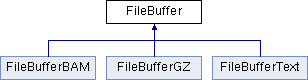
\includegraphics[height=2.000000cm]{classFileBuffer}
\end{center}
\end{figure}
\subsection*{Public Member Functions}
\begin{DoxyCompactItemize}
\item 
\hypertarget{classFileBuffer_ab243cfcb8a68ce791103594e974ee9ba}{
\hyperlink{classFileBuffer_ab243cfcb8a68ce791103594e974ee9ba}{FileBuffer} ()}
\label{classFileBuffer_ab243cfcb8a68ce791103594e974ee9ba}

\begin{DoxyCompactList}\small\item\em Empty class constructor. \end{DoxyCompactList}\item 
\hypertarget{classFileBuffer_ac92d5e7d145ea18fc6a3a6a18c788ebb}{
virtual \hyperlink{classFileBuffer_ac92d5e7d145ea18fc6a3a6a18c788ebb}{$\sim$FileBuffer} ()}
\label{classFileBuffer_ac92d5e7d145ea18fc6a3a6a18c788ebb}

\begin{DoxyCompactList}\small\item\em Class destructor. \end{DoxyCompactList}\item 
\hypertarget{classFileBuffer_a83e9378412806c2646639d2b4c7c457f}{
long int \hyperlink{classFileBuffer_a83e9378412806c2646639d2b4c7c457f}{CountLines} ()}
\label{classFileBuffer_a83e9378412806c2646639d2b4c7c457f}

\begin{DoxyCompactList}\small\item\em Counts the number of lines in the file. \end{DoxyCompactList}\item 
\hypertarget{classFileBuffer_ad460e02c3739484feb72e40bff60a09d}{
virtual void \hyperlink{classFileBuffer_ad460e02c3739484feb72e40bff60a09d}{Reset} ()=0}
\label{classFileBuffer_ad460e02c3739484feb72e40bff60a09d}

\begin{DoxyCompactList}\small\item\em Resets the file pointer (obviously this does not work for standard input) \end{DoxyCompactList}\item 
\hypertarget{classFileBuffer_a48bf46db592b676a68cc33dc10a0e272}{
char $\ast$ \hyperlink{classFileBuffer_a48bf46db592b676a68cc33dc10a0e272}{Get} ()}
\label{classFileBuffer_a48bf46db592b676a68cc33dc10a0e272}

\begin{DoxyCompactList}\small\item\em Returns a pointer to the current line. \end{DoxyCompactList}\item 
\hypertarget{classFileBuffer_a5b6e4589577674a2202be410aebd847d}{
virtual char $\ast$ \hyperlink{classFileBuffer_a5b6e4589577674a2202be410aebd847d}{Next} ()=0}
\label{classFileBuffer_a5b6e4589577674a2202be410aebd847d}

\begin{DoxyCompactList}\small\item\em Read the next line. \end{DoxyCompactList}\end{DoxyCompactItemize}
\subsection*{Public Attributes}
\begin{DoxyCompactItemize}
\item 
\hypertarget{classFileBuffer_a8e4c0122ac4352e5a930248f982da2ca}{
bool \hyperlink{classFileBuffer_a8e4c0122ac4352e5a930248f982da2ca}{is\_\-stdin}}
\label{classFileBuffer_a8e4c0122ac4352e5a930248f982da2ca}

\begin{DoxyCompactList}\small\item\em true if reading from standard input \end{DoxyCompactList}\item 
\hypertarget{classFileBuffer_ab91de85b7f0eab77697c680346c4f61d}{
unsigned long int \hyperlink{classFileBuffer_ab91de85b7f0eab77697c680346c4f61d}{n\_\-line}}
\label{classFileBuffer_ab91de85b7f0eab77697c680346c4f61d}

\begin{DoxyCompactList}\small\item\em keeps track of line number \end{DoxyCompactList}\item 
\hypertarget{classFileBuffer_a416474b62bf29cc6e44dbb3d7db5fb2a}{
char $\ast$ \hyperlink{classFileBuffer_a416474b62bf29cc6e44dbb3d7db5fb2a}{file\_\-name}}
\label{classFileBuffer_a416474b62bf29cc6e44dbb3d7db5fb2a}

\begin{DoxyCompactList}\small\item\em file name \end{DoxyCompactList}\item 
\hypertarget{classFileBuffer_af93bf5b014aac504fca11ab6a2d59fb0}{
char $\ast$ \hyperlink{classFileBuffer_af93bf5b014aac504fca11ab6a2d59fb0}{BUFFER}}
\label{classFileBuffer_af93bf5b014aac504fca11ab6a2d59fb0}

\begin{DoxyCompactList}\small\item\em where input line is stored \end{DoxyCompactList}\item 
\hypertarget{classFileBuffer_a73d2b90a38cc6e8326fbc03b7ff244ef}{
unsigned long int \hyperlink{classFileBuffer_a73d2b90a38cc6e8326fbc03b7ff244ef}{BUFFER\_\-SIZE}}
\label{classFileBuffer_a73d2b90a38cc6e8326fbc03b7ff244ef}

\begin{DoxyCompactList}\small\item\em buffer size (automatically adjusted during execution to accommodate any line size) \end{DoxyCompactList}\end{DoxyCompactItemize}


\subsection{Detailed Description}
Abstract class for reading lines from file. 

The documentation for this class was generated from the following files:\begin{DoxyCompactItemize}
\item 
core.h\item 
core.cpp\end{DoxyCompactItemize}

\hypertarget{classGenomicInterval}{
\section{GenomicInterval Class Reference}
\label{classGenomicInterval}\index{GenomicInterval@{GenomicInterval}}
}
set of CIGAR operations that map to the fragment sequence (SAM format)  


{\tt \#include $<$genomic\_\-intervals.h$>$}

\subsection*{Public Member Functions}
\begin{CompactItemize}
\item 
\hypertarget{classGenomicInterval_09dcaee742ca117a8caaa1c656d0e354}{
\hyperlink{classGenomicInterval_09dcaee742ca117a8caaa1c656d0e354}{GenomicInterval} (char $\ast$chromosome, char strand, long int start, long int stop, unsigned long int \hyperlink{classGenomicInterval_0dbe6195570468c386eea923e30c762c}{n\_\-line}=0)}
\label{classGenomicInterval_09dcaee742ca117a8caaa1c656d0e354}

\begin{CompactList}\small\item\em Class constructor, see example below. \item\end{CompactList}\item 
\hypertarget{classGenomicInterval_c452f2239b17bc72efe4eef12a261514}{
\hyperlink{classGenomicInterval_c452f2239b17bc72efe4eef12a261514}{GenomicInterval} (string chromosome, char strand, long int start, long int stop, unsigned long int \hyperlink{classGenomicInterval_0dbe6195570468c386eea923e30c762c}{n\_\-line}=0)}
\label{classGenomicInterval_c452f2239b17bc72efe4eef12a261514}

\begin{CompactList}\small\item\em Class constructor, see example below. \item\end{CompactList}\item 
\hypertarget{classGenomicInterval_99f413828468dca1eeb5cc806848d98e}{
\hyperlink{classGenomicInterval_99f413828468dca1eeb5cc806848d98e}{GenomicInterval} (char $\ast$inp, char delimiter=' ', unsigned long int \hyperlink{classGenomicInterval_0dbe6195570468c386eea923e30c762c}{n\_\-line}=0)}
\label{classGenomicInterval_99f413828468dca1eeb5cc806848d98e}

\begin{CompactList}\small\item\em Class constructor, see example below. \item\end{CompactList}\item 
\hypertarget{classGenomicInterval_4132f8d27fa5ebe416abe41150974c14}{
\hyperlink{classGenomicInterval_4132f8d27fa5ebe416abe41150974c14}{GenomicInterval} (\hyperlink{classGenomicInterval}{GenomicInterval} $\ast$I)}
\label{classGenomicInterval_4132f8d27fa5ebe416abe41150974c14}

\begin{CompactList}\small\item\em Class constructor, see example below. \item\end{CompactList}\item 
\hypertarget{classGenomicInterval_632a255d16cb13b15b2f2d4f826cace7}{
\hyperlink{classGenomicInterval_632a255d16cb13b15b2f2d4f826cace7}{$\sim$GenomicInterval} ()}
\label{classGenomicInterval_632a255d16cb13b15b2f2d4f826cace7}

\begin{CompactList}\small\item\em Class Destructor. \item\end{CompactList}\item 
\hypertarget{classGenomicInterval_feba30dc21d2e5ed7e460eb1b79f021b}{
void \hyperlink{classGenomicInterval_feba30dc21d2e5ed7e460eb1b79f021b}{PrintInterval} ()}
\label{classGenomicInterval_feba30dc21d2e5ed7e460eb1b79f021b}

\begin{CompactList}\small\item\em Print interval (do not print newline character). \item\end{CompactList}\item 
\hypertarget{classGenomicInterval_968607fbfe88e86760924156f6519d98}{
void \hyperlink{classGenomicInterval_968607fbfe88e86760924156f6519d98}{PrintInterval} (FILE $\ast$file\_\-ptr)}
\label{classGenomicInterval_968607fbfe88e86760924156f6519d98}

\begin{CompactList}\small\item\em Print interval in file (do not print newline character). \item\end{CompactList}\item 
\hypertarget{classGenomicInterval_310800040ea4e328f5899611143caee0}{
void \hyperlink{classGenomicInterval_310800040ea4e328f5899611143caee0}{PrintInterval} (long int start, long int stop)}
\label{classGenomicInterval_310800040ea4e328f5899611143caee0}

\begin{CompactList}\small\item\em Print interval with modified start and stop positions (do not print newline character). \item\end{CompactList}\item 
\hypertarget{classGenomicInterval_70f300009a0cc29b024853fb794d0e9a}{
void \hyperlink{classGenomicInterval_70f300009a0cc29b024853fb794d0e9a}{Print} (bool point=false)}
\label{classGenomicInterval_70f300009a0cc29b024853fb794d0e9a}

\begin{CompactList}\small\item\em Print interval with a newline character at the end. If {\bf point} is 'true', then print every point in the interval separately. \item\end{CompactList}\item 
\hypertarget{classGenomicInterval_dbd1571cf6db0ef646f9b1e095bfcb4e}{
void \hyperlink{classGenomicInterval_dbd1571cf6db0ef646f9b1e095bfcb4e}{PrintWithLabel} (char $\ast$label, bool point=false)}
\label{classGenomicInterval_dbd1571cf6db0ef646f9b1e095bfcb4e}

\begin{CompactList}\small\item\em Print interval with a label in front and newline character at the end. \item\end{CompactList}\item 
\hypertarget{classGenomicInterval_79d1e06f62b4c1eddda7b9fc62733c7b}{
bool \hyperlink{classGenomicInterval_79d1e06f62b4c1eddda7b9fc62733c7b}{IsValid} ()}
\label{classGenomicInterval_79d1e06f62b4c1eddda7b9fc62733c7b}

\begin{CompactList}\small\item\em Check integrity of interval start/stop positions (start$>$=1 and stop$>$=start). \item\end{CompactList}\item 
\hypertarget{classGenomicInterval_b9323c2818c13a25fda953ae18fc97aa}{
bool \hyperlink{classGenomicInterval_b9323c2818c13a25fda953ae18fc97aa}{CheckValid} (bool quiet=false)}
\label{classGenomicInterval_b9323c2818c13a25fda953ae18fc97aa}

\begin{CompactList}\small\item\em Same as \hyperlink{classGenomicInterval_79d1e06f62b4c1eddda7b9fc62733c7b}{GenomicInterval::IsValid}, but it also prints error messages. \item\end{CompactList}\item 
\hypertarget{classGenomicInterval_36dc2d4059337cc03a1211b6b8a7471c}{
bool \hyperlink{classGenomicInterval_36dc2d4059337cc03a1211b6b8a7471c}{IsBefore} (\hyperlink{classGenomicInterval}{GenomicInterval} $\ast$I, bool sorted\_\-by\_\-strand)}
\label{classGenomicInterval_36dc2d4059337cc03a1211b6b8a7471c}

\begin{CompactList}\small\item\em Compares with input interval {\bf I} and returns true if its order is before {\bf I}. The order is determined first by chromosome, then by strand, and finally by start position. \item\end{CompactList}\item 
\hypertarget{classGenomicInterval_8fc5d344a103f145db968e536b30f9cf}{
bool \hyperlink{classGenomicInterval_8fc5d344a103f145db968e536b30f9cf}{IsPosBefore} (\hyperlink{classGenomicInterval}{GenomicInterval} $\ast$I)}
\label{classGenomicInterval_8fc5d344a103f145db968e536b30f9cf}

\begin{CompactList}\small\item\em Compares with input interval {\bf I} and returns true if its position order is before {\bf I}. The position order is determined first by start position and then by stop position. \item\end{CompactList}\item 
\hypertarget{classGenomicInterval_b6febc4c04d4919a9485ce8eeec5129d}{
bool \hyperlink{classGenomicInterval_b6febc4c04d4919a9485ce8eeec5129d}{IsCompatibleWith} (\hyperlink{classGenomicInterval}{GenomicInterval} $\ast$I, bool ignore\_\-strand)}
\label{classGenomicInterval_b6febc4c04d4919a9485ce8eeec5129d}

\begin{CompactList}\small\item\em Compares with input interval {\bf I} and returns true if intervals are in the same chromosome and strand. \item\end{CompactList}\item 
\hypertarget{classGenomicInterval_a1c591b6d3cc3c576cec24a3ab67abfb}{
bool \hyperlink{classGenomicInterval_a1c591b6d3cc3c576cec24a3ab67abfb}{OverlapsWith} (\hyperlink{classGenomicInterval}{GenomicInterval} $\ast$I, bool ignore\_\-strand=false)}
\label{classGenomicInterval_a1c591b6d3cc3c576cec24a3ab67abfb}

\begin{CompactList}\small\item\em Returns 'true' if it overlaps with input interval {\bf I}. \item\end{CompactList}\item 
\hypertarget{classGenomicInterval_c76f5c0d3cae831f6cec9d8a27b1c56d}{
void \hyperlink{classGenomicInterval_c76f5c0d3cae831f6cec9d8a27b1c56d}{SetCoordinates} (long int start, long int stop)}
\label{classGenomicInterval_c76f5c0d3cae831f6cec9d8a27b1c56d}

\begin{CompactList}\small\item\em Set start/stop positions to new values. \item\end{CompactList}\item 
\hypertarget{classGenomicInterval_e068e54e894fb239b61ec6d29e5f70bf}{
long int \hyperlink{classGenomicInterval_e068e54e894fb239b61ec6d29e5f70bf}{GetCoordinate} (char $\ast$op)}
\label{classGenomicInterval_e068e54e894fb239b61ec6d29e5f70bf}

\begin{CompactList}\small\item\em If: op='1' returns start position, op='2' returns stop position, op='5p' returns 5-prime, op='3p' returns 3-prime. \item\end{CompactList}\item 
\hypertarget{classGenomicInterval_7ceb36d952453db9473c7548c885f40a}{
size\_\-t \hyperlink{classGenomicInterval_7ceb36d952453db9473c7548c885f40a}{GetSize} ()}
\label{classGenomicInterval_7ceb36d952453db9473c7548c885f40a}

\begin{CompactList}\small\item\em Returns interval size. \item\end{CompactList}\item 
\hypertarget{classGenomicInterval_ff25b35226220508539b1183d5b9c11d}{
char $\ast$ \hyperlink{classGenomicInterval_ff25b35226220508539b1183d5b9c11d}{GetSeq} (\hyperlink{classChromosomes}{Chromosomes} $\ast$C, bool replace=false)}
\label{classGenomicInterval_ff25b35226220508539b1183d5b9c11d}

\begin{CompactList}\small\item\em Extracts genomic interval sequence from chromosomal sequences supplied in {\bf C}. If parameter {\bf replace} is true, it replaces \char`\"{}N\char`\"{} with lowercase \char`\"{}a\char`\"{}. \item\end{CompactList}\item 
\hypertarget{classGenomicInterval_39cd65d08a0c64a8bbddec32c8decbd3}{
size\_\-t \hyperlink{classGenomicInterval_39cd65d08a0c64a8bbddec32c8decbd3}{GetSeqLength} (\hyperlink{classChromosomes}{Chromosomes} $\ast$C)}
\label{classGenomicInterval_39cd65d08a0c64a8bbddec32c8decbd3}

\begin{CompactList}\small\item\em Returns sequence length excluding 'N' characters. \item\end{CompactList}\item 
\hypertarget{classGenomicInterval_ea112f495d21eda675de671d9ff2e5ad}{
long int \hyperlink{classGenomicInterval_ea112f495d21eda675de671d9ff2e5ad}{CalcOverlap} (\hyperlink{classGenomicInterval}{GenomicInterval} $\ast$I, bool ignore\_\-strand)}
\label{classGenomicInterval_ea112f495d21eda675de671d9ff2e5ad}

\begin{CompactList}\small\item\em Calculates the overlap with input interval {\bf I}. \item\end{CompactList}\item 
\hypertarget{classGenomicInterval_a801336aa07a0029d97d7914a747abd3}{
long int \hyperlink{classGenomicInterval_a801336aa07a0029d97d7914a747abd3}{CalcDistanceFrom} (\hyperlink{classGenomicInterval}{GenomicInterval} $\ast$I, char $\ast$op, char $\ast$I\_\-op)}
\label{classGenomicInterval_a801336aa07a0029d97d7914a747abd3}

\begin{CompactList}\small\item\em Calculates the distance from input interval {\bf I} based on position operators {\bf op} and {\bf I\_\-op}. \item\end{CompactList}\item 
\hypertarget{classGenomicInterval_7856012eda653222a1ac5482510bacc7}{
int \hyperlink{classGenomicInterval_7856012eda653222a1ac5482510bacc7}{CalcDirection} (\hyperlink{classGenomicInterval}{GenomicInterval} $\ast$i, bool sorted\_\-by\_\-strand)}
\label{classGenomicInterval_7856012eda653222a1ac5482510bacc7}

\begin{CompactList}\small\item\em Returns -1 if before interval {\bf i}, +1 if after, and 0 if the intervals overlap. The order is determined first by chromosome, then (optionally) by strand and finally by start position. \item\end{CompactList}\item 
\hypertarget{classGenomicInterval_b14f526a4df4f148e1b843ee0dc10d04}{
void \hyperlink{classGenomicInterval_b14f526a4df4f148e1b843ee0dc10d04}{PrintSeq} (\hyperlink{classChromosomes}{Chromosomes} $\ast$C, bool replace=false)}
\label{classGenomicInterval_b14f526a4df4f148e1b843ee0dc10d04}

\begin{CompactList}\small\item\em Prints genomic interval sequence from chromosomal sequences supplied in {\bf C}. If parameter {\bf replace} is true, it replaces \char`\"{}N\char`\"{} with lowercase \char`\"{}a\char`\"{}. \item\end{CompactList}\item 
\hypertarget{classGenomicInterval_a410816fa04d76edd7caeb9ae2442ae1}{
void \hyperlink{classGenomicInterval_a410816fa04d76edd7caeb9ae2442ae1}{ReverseStrand} ()}
\label{classGenomicInterval_a410816fa04d76edd7caeb9ae2442ae1}

\begin{CompactList}\small\item\em If interval strand is '+', it is changed to '-' and vice versa. \item\end{CompactList}\item 
void \hyperlink{classGenomicInterval_5cc57eb991cca3f1e1b8bd7ca8acaa03}{ShiftPos} (long int start\_\-shift, long int stop\_\-shift, bool shift\_\-5prime)
\begin{CompactList}\small\item\em Shifts interval start/stop positions. First it chooses reference position, and then shifts start and stop positions separately. \item\end{CompactList}\item 
void \hyperlink{classGenomicInterval_96b34b76019001c4751d4c4f868ee24d}{ModifyPos} (char $\ast$position\_\-op, long int position\_\-shift)
\begin{CompactList}\small\item\em Modifies interval start/stop positions. First it chooses which position to keep fixed, and then it shifts the non-fixed position. \item\end{CompactList}\item 
\hypertarget{classGenomicInterval_bf416450f25b579dfb76b2bd6a81aa6a}{
void \hyperlink{classGenomicInterval_bf416450f25b579dfb76b2bd6a81aa6a}{ReversePos} (StringLIntMap $\ast$bounds)}
\label{classGenomicInterval_bf416450f25b579dfb76b2bd6a81aa6a}

\begin{CompactList}\small\item\em Reverses interval start/stop positions with respect to chromosomal bounds, as if the reference point were in the end of the chromosome as opposed to the beginning. \item\end{CompactList}\item 
\hypertarget{classGenomicInterval_1834c0f1217585398de74119d680ab7b}{
bool \hyperlink{classGenomicInterval_1834c0f1217585398de74119d680ab7b}{CheckBounds} (StringLIntMap $\ast$bounds, bool ignore)}
\label{classGenomicInterval_1834c0f1217585398de74119d680ab7b}

\begin{CompactList}\small\item\em Checks if interval start/stop positions comply with chromosomal bounds. \item\end{CompactList}\item 
\hypertarget{classGenomicInterval_c28099b569624adcf3b327e922e5e4e5}{
void \hyperlink{classGenomicInterval_c28099b569624adcf3b327e922e5e4e5}{ApplyBounds} (StringLIntMap $\ast$bounds)}
\label{classGenomicInterval_c28099b569624adcf3b327e922e5e4e5}

\begin{CompactList}\small\item\em Corrects interval start/stop positions so as to comply with chromosomal bounds. \item\end{CompactList}\item 
\hypertarget{classGenomicInterval_c06925f3fcf6b47cec5c6f95aaa379c0}{
void \hyperlink{classGenomicInterval_c06925f3fcf6b47cec5c6f95aaa379c0}{PrintBEDFormat} (char $\ast$color, bool convert\_\-chromosome)}
\label{classGenomicInterval_c06925f3fcf6b47cec5c6f95aaa379c0}

\begin{CompactList}\small\item\em Prints in BED format. If {\bf convert\_\-chromosome} is 'true', then convert from ENSEMBL to UCSC names (by adding 'chr' prefix to each chromosome name, and by converting 'MT' to 'chrM'). \item\end{CompactList}\item 
\hypertarget{classGenomicInterval_75aed02c1df83acb5d7ec89e2a9949bd}{
void \hyperlink{classGenomicInterval_75aed02c1df83acb5d7ec89e2a9949bd}{Randomize} (gsl\_\-rng $\ast$random\_\-generator, StringLIntMap $\ast$bounds)}
\label{classGenomicInterval_75aed02c1df83acb5d7ec89e2a9949bd}

\begin{CompactList}\small\item\em Randomizes interval position within chromosomal bounds. \item\end{CompactList}\item 
void \hyperlink{classGenomicInterval_ab40ad7dd997948e0c04a13164e955d6}{GetOffsetFrom} (\hyperlink{classGenomicInterval}{GenomicInterval} $\ast$ReferenceI, char $\ast$op, bool ignore\_\-strand, long int $\ast$start\_\-offset, long int $\ast$stop\_\-offset)
\begin{CompactList}\small\item\em Computes start/stop offset distances from {\bf ReferenceI}. \item\end{CompactList}\end{CompactItemize}
\subsection*{Public Attributes}
\begin{CompactItemize}
\item 
\hypertarget{classGenomicInterval_0dbe6195570468c386eea923e30c762c}{
unsigned long int \hyperlink{classGenomicInterval_0dbe6195570468c386eea923e30c762c}{n\_\-line}}
\label{classGenomicInterval_0dbe6195570468c386eea923e30c762c}

\begin{CompactList}\small\item\em file line number \item\end{CompactList}\item 
\hypertarget{classGenomicInterval_c489a1195c43cc93d0e192dc91d5a192}{
char $\ast$ \hyperlink{classGenomicInterval_c489a1195c43cc93d0e192dc91d5a192}{CHROMOSOME}}
\label{classGenomicInterval_c489a1195c43cc93d0e192dc91d5a192}

\begin{CompactList}\small\item\em chromosome name (space and tab characters are not allowed) \item\end{CompactList}\item 
\hypertarget{classGenomicInterval_25f6603b48fcc57f97c89fa768b658f9}{
char \hyperlink{classGenomicInterval_25f6603b48fcc57f97c89fa768b658f9}{STRAND}}
\label{classGenomicInterval_25f6603b48fcc57f97c89fa768b658f9}

\begin{CompactList}\small\item\em orientation ('+' or '-') \item\end{CompactList}\item 
\hypertarget{classGenomicInterval_c0abba93599f5cdf4b5a4e7ec5909bbd}{
long int \hyperlink{classGenomicInterval_c0abba93599f5cdf4b5a4e7ec5909bbd}{START}}
\label{classGenomicInterval_c0abba93599f5cdf4b5a4e7ec5909bbd}

\begin{CompactList}\small\item\em interval start position in the chromosome ($>$=1) \item\end{CompactList}\item 
\hypertarget{classGenomicInterval_c5fac21da3939b7976859a54800b93f0}{
long int \hyperlink{classGenomicInterval_c5fac21da3939b7976859a54800b93f0}{STOP}}
\label{classGenomicInterval_c5fac21da3939b7976859a54800b93f0}

\begin{CompactList}\small\item\em interval stop position in the chromosome ($<$=chromosome\_\-size) \item\end{CompactList}\end{CompactItemize}


\subsection{Detailed Description}
set of CIGAR operations that map to the fragment sequence (SAM format) 

This class implements the genomic interval.

Genomic intervals can be constructed from strings that follow this format:

CHROMOSOME {\em $<$SPACE$>$\/} STRAND {\em $<$SPACE$>$\/} START {\em $<$SPACE$>$\/} STOP

Example: 

\begin{Code}\begin{verbatim}    GenomicInterval x("chr1",'+',132034,135932);
    GenomicInterval y("chr1 + 135832 140102");
    cout << "size of interval x = " << x.GetSize() << '\n';
    cout << "size of interval y = " << y.GetSize() << '\n';
    cout << "overlap of x and y = " << x.GetOverlap(&y) << '\n';    
\end{verbatim}
\end{Code}

 

\subsection{Member Function Documentation}
\hypertarget{classGenomicInterval_5cc57eb991cca3f1e1b8bd7ca8acaa03}{
\index{GenomicInterval@{GenomicInterval}!ShiftPos@{ShiftPos}}
\index{ShiftPos@{ShiftPos}!GenomicInterval@{GenomicInterval}}
\subsubsection[ShiftPos]{\setlength{\rightskip}{0pt plus 5cm}void GenomicInterval::ShiftPos (long int {\em start\_\-shift}, \/  long int {\em stop\_\-shift}, \/  bool {\em shift\_\-5prime})}}
\label{classGenomicInterval_5cc57eb991cca3f1e1b8bd7ca8acaa03}


Shifts interval start/stop positions. First it chooses reference position, and then shifts start and stop positions separately. 

\begin{Desc}
\item[Parameters:]
\begin{description}
\item[{\em start\_\-shift}]determines the shift of the start position \item[{\em stop\_\-shift}]determines the shift of the stop position \item[{\em shift\_\-5prime}]if 'true', then the new start position is the old 5-prime position shifted by {\bf start\_\-shift} and the new stop position is the old 3-prime position shifted by {\bf stop\_\-shift} \end{description}
\end{Desc}
\hypertarget{classGenomicInterval_96b34b76019001c4751d4c4f868ee24d}{
\index{GenomicInterval@{GenomicInterval}!ModifyPos@{ModifyPos}}
\index{ModifyPos@{ModifyPos}!GenomicInterval@{GenomicInterval}}
\subsubsection[ModifyPos]{\setlength{\rightskip}{0pt plus 5cm}void GenomicInterval::ModifyPos (char $\ast$ {\em position\_\-op}, \/  long int {\em position\_\-shift})}}
\label{classGenomicInterval_96b34b76019001c4751d4c4f868ee24d}


Modifies interval start/stop positions. First it chooses which position to keep fixed, and then it shifts the non-fixed position. 

\begin{Desc}
\item[Parameters:]
\begin{description}
\item[{\em position\_\-op}]selects fixed position as follows: '1'=start position, 'c'=center position, '5p'=5-prime, '3p'=3-prime \item[{\em position\_\-shift}]determines the shift of the non-fixed position (in the 'c' case, both positions are shifted symmetrically around the center) \end{description}
\end{Desc}
\hypertarget{classGenomicInterval_ab40ad7dd997948e0c04a13164e955d6}{
\index{GenomicInterval@{GenomicInterval}!GetOffsetFrom@{GetOffsetFrom}}
\index{GetOffsetFrom@{GetOffsetFrom}!GenomicInterval@{GenomicInterval}}
\subsubsection[GetOffsetFrom]{\setlength{\rightskip}{0pt plus 5cm}void GenomicInterval::GetOffsetFrom ({\bf GenomicInterval} $\ast$ {\em ReferenceI}, \/  char $\ast$ {\em op}, \/  bool {\em ignore\_\-strand}, \/  long int $\ast$ {\em start\_\-offset}, \/  long int $\ast$ {\em stop\_\-offset})}}
\label{classGenomicInterval_ab40ad7dd997948e0c04a13164e955d6}


Computes start/stop offset distances from {\bf ReferenceI}. 

\begin{Desc}
\item[Parameters:]
\begin{description}
\item[{\em ReferenceI}]pointer to reference interval \item[{\em op}]selects reference point: '1'=start position, '2'=stop position, '5p'=5-prime position, '3p'=3-prime position \item[{\em ignore\_\-strand}]ignore mismatch between test and reference strand \item[{\em start\_\-offset}]return value: the start offset \item[{\em stop\_\-offset}]return value: the stop offset \end{description}
\end{Desc}


The documentation for this class was generated from the following files:\begin{CompactItemize}
\item 
genomic\_\-intervals.h\item 
genomic\_\-intervals.cpp\end{CompactItemize}

\hypertarget{classGenomicIntervalSetAsArray}{
\section{GenomicIntervalSetAsArray Class Reference}
\label{classGenomicIntervalSetAsArray}\index{GenomicIntervalSetAsArray@{GenomicIntervalSetAsArray}}
}
\mbox{[}UNDER DEVELOPMENT\mbox{]} This class implements an array of genomic intervals.  


{\tt \#include $<$genomic\_\-intervals.h$>$}

\subsection*{Public Types}
\begin{CompactItemize}
\item 
\hypertarget{classGenomicIntervalSetAsArray_1a0416c9fac7e9d965ae7fe84f1649c2}{
typedef \hyperlink{classGenomicInterval}{GenomicInterval} $\ast$$\ast$ \hyperlink{classGenomicIntervalSetAsArray_1a0416c9fac7e9d965ae7fe84f1649c2}{iterator}}
\label{classGenomicIntervalSetAsArray_1a0416c9fac7e9d965ae7fe84f1649c2}

\begin{CompactList}\small\item\em iterator defined as a pointer in the array of \hyperlink{classGenomicInterval}{GenomicInterval} \item\end{CompactList}\item 
\hypertarget{classGenomicIntervalSetAsArray_0310f5d79c529b631a5ef71ef186b41c}{
typedef \hyperlink{classGenomicInterval}{GenomicInterval} $\ast$$\ast$ \hyperlink{classGenomicIntervalSetAsArray_0310f5d79c529b631a5ef71ef186b41c}{reverse\_\-iterator}}
\label{classGenomicIntervalSetAsArray_0310f5d79c529b631a5ef71ef186b41c}

\begin{CompactList}\small\item\em reverse\_\-iterator defined as a pointer in the array of \hyperlink{classGenomicInterval}{GenomicInterval} \item\end{CompactList}\end{CompactItemize}
\subsection*{Public Member Functions}
\begin{CompactItemize}
\item 
\hypertarget{classGenomicIntervalSetAsArray_12686a38ae225b2794feb5a3ef1f4430}{
\hyperlink{classGenomicIntervalSetAsArray_12686a38ae225b2794feb5a3ef1f4430}{GenomicIntervalSetAsArray} ()}
\label{classGenomicIntervalSetAsArray_12686a38ae225b2794feb5a3ef1f4430}

\begin{CompactList}\small\item\em Empty class constructor. \item\end{CompactList}\item 
\hypertarget{classGenomicIntervalSetAsArray_05dafd13fef5a9db6339db5c103fef23}{
\hyperlink{classGenomicIntervalSetAsArray_05dafd13fef5a9db6339db5c103fef23}{$\sim$GenomicIntervalSetAsArray} ()}
\label{classGenomicIntervalSetAsArray_05dafd13fef5a9db6339db5c103fef23}

\begin{CompactList}\small\item\em Class destructor. \item\end{CompactList}\item 
\hypertarget{classGenomicIntervalSetAsArray_9e56381009d164d7625199b183845388}{
\hyperlink{classGenomicInterval}{iterator} \hyperlink{classGenomicIntervalSetAsArray_9e56381009d164d7625199b183845388}{begin} ()}
\label{classGenomicIntervalSetAsArray_9e56381009d164d7625199b183845388}

\begin{CompactList}\small\item\em Implementation of \hyperlink{classGenomicIntervalSetAsArray_9e56381009d164d7625199b183845388}{begin()} for this container. \item\end{CompactList}\item 
\hypertarget{classGenomicIntervalSetAsArray_5b6145ceff99907d9075047519482584}{
\hyperlink{classGenomicInterval}{iterator} \hyperlink{classGenomicIntervalSetAsArray_5b6145ceff99907d9075047519482584}{end} ()}
\label{classGenomicIntervalSetAsArray_5b6145ceff99907d9075047519482584}

\begin{CompactList}\small\item\em Implementation of \hyperlink{classGenomicIntervalSetAsArray_5b6145ceff99907d9075047519482584}{end()} for this container. \item\end{CompactList}\item 
\hypertarget{classGenomicIntervalSetAsArray_c077589a55a7dfec9b2e6c38392f7444}{
\hyperlink{classGenomicInterval}{iterator} \hyperlink{classGenomicIntervalSetAsArray_c077589a55a7dfec9b2e6c38392f7444}{rbegin} ()}
\label{classGenomicIntervalSetAsArray_c077589a55a7dfec9b2e6c38392f7444}

\begin{CompactList}\small\item\em Implementation of \hyperlink{classGenomicIntervalSetAsArray_c077589a55a7dfec9b2e6c38392f7444}{rbegin()} for this container. \item\end{CompactList}\item 
\hypertarget{classGenomicIntervalSetAsArray_5b7fc7dc64857dfdadd1198393c0d117}{
\hyperlink{classGenomicInterval}{iterator} \hyperlink{classGenomicIntervalSetAsArray_5b7fc7dc64857dfdadd1198393c0d117}{rend} ()}
\label{classGenomicIntervalSetAsArray_5b7fc7dc64857dfdadd1198393c0d117}

\begin{CompactList}\small\item\em Implementation of \hyperlink{classGenomicIntervalSetAsArray_5b7fc7dc64857dfdadd1198393c0d117}{rend()} for this container. \item\end{CompactList}\item 
\hypertarget{classGenomicIntervalSetAsArray_a74747b36b114c326edfaf1224270d0d}{
\hyperlink{classGenomicInterval}{GenomicInterval} $\ast$ \hyperlink{classGenomicIntervalSetAsArray_a74747b36b114c326edfaf1224270d0d}{front} ()}
\label{classGenomicIntervalSetAsArray_a74747b36b114c326edfaf1224270d0d}

\begin{CompactList}\small\item\em Implementation of \hyperlink{classGenomicIntervalSetAsArray_a74747b36b114c326edfaf1224270d0d}{front()} for this container. \item\end{CompactList}\item 
\hypertarget{classGenomicIntervalSetAsArray_11b483c12111ee96c15fec296c66ee15}{
\hyperlink{classGenomicInterval}{GenomicInterval} $\ast$ \hyperlink{classGenomicIntervalSetAsArray_11b483c12111ee96c15fec296c66ee15}{back} ()}
\label{classGenomicIntervalSetAsArray_11b483c12111ee96c15fec296c66ee15}

\begin{CompactList}\small\item\em Implementation of \hyperlink{classGenomicIntervalSetAsArray_11b483c12111ee96c15fec296c66ee15}{back()} for this container. \item\end{CompactList}\item 
\hypertarget{classGenomicIntervalSetAsArray_d4bfef55744241849841c71d08835403}{
size\_\-t \hyperlink{classGenomicIntervalSetAsArray_d4bfef55744241849841c71d08835403}{size} ()}
\label{classGenomicIntervalSetAsArray_d4bfef55744241849841c71d08835403}

\begin{CompactList}\small\item\em Implementation of \hyperlink{classGenomicIntervalSetAsArray_d4bfef55744241849841c71d08835403}{size()} for this container. \item\end{CompactList}\item 
\hypertarget{classGenomicIntervalSetAsArray_4348e7636cb91405b08374a966e33a7c}{
void \hyperlink{classGenomicIntervalSetAsArray_4348e7636cb91405b08374a966e33a7c}{push\_\-back} (\hyperlink{classGenomicInterval}{GenomicInterval} $\ast$j)}
\label{classGenomicIntervalSetAsArray_4348e7636cb91405b08374a966e33a7c}

\begin{CompactList}\small\item\em Implementation of \hyperlink{classGenomicIntervalSetAsArray_4348e7636cb91405b08374a966e33a7c}{push\_\-back()} for this container. \item\end{CompactList}\item 
\hypertarget{classGenomicIntervalSetAsArray_833395eaf9daa5626879eefa861d9ea5}{
void \hyperlink{classGenomicIntervalSetAsArray_833395eaf9daa5626879eefa861d9ea5}{clear} ()}
\label{classGenomicIntervalSetAsArray_833395eaf9daa5626879eefa861d9ea5}

\begin{CompactList}\small\item\em Implementation of \hyperlink{classGenomicIntervalSetAsArray_833395eaf9daa5626879eefa861d9ea5}{clear()} for this container. \item\end{CompactList}\item 
\hypertarget{classGenomicIntervalSetAsArray_0f8554cfca150d695d15691aa42df7fa}{
\hyperlink{classGenomicInterval}{iterator} \hyperlink{classGenomicIntervalSetAsArray_0f8554cfca150d695d15691aa42df7fa}{erase} (\hyperlink{classGenomicInterval}{iterator} i, \hyperlink{classGenomicInterval}{iterator} j)}
\label{classGenomicIntervalSetAsArray_0f8554cfca150d695d15691aa42df7fa}

\begin{CompactList}\small\item\em Implementation of \hyperlink{classGenomicIntervalSetAsArray_0f8554cfca150d695d15691aa42df7fa}{erase()} for this container (exits with error message). \item\end{CompactList}\item 
\hypertarget{classGenomicIntervalSetAsArray_0aae25ac2e9a7cf50a370703aa99df85}{
\hyperlink{classGenomicInterval}{iterator} \hyperlink{classGenomicIntervalSetAsArray_0aae25ac2e9a7cf50a370703aa99df85}{erase} (\hyperlink{classGenomicInterval}{iterator} i)}
\label{classGenomicIntervalSetAsArray_0aae25ac2e9a7cf50a370703aa99df85}

\begin{CompactList}\small\item\em Implementation of \hyperlink{classGenomicIntervalSetAsArray_0f8554cfca150d695d15691aa42df7fa}{erase()} for this container (exits with error message). \item\end{CompactList}\item 
\hypertarget{classGenomicIntervalSetAsArray_0cd89244c0e75b88f9b56c9b9478d06b}{
\hyperlink{classGenomicInterval}{iterator} \hyperlink{classGenomicIntervalSetAsArray_0cd89244c0e75b88f9b56c9b9478d06b}{insert} (\hyperlink{classGenomicInterval}{iterator} i, \hyperlink{classGenomicInterval}{GenomicInterval} $\ast$u)}
\label{classGenomicIntervalSetAsArray_0cd89244c0e75b88f9b56c9b9478d06b}

\begin{CompactList}\small\item\em Implementation of \hyperlink{classGenomicIntervalSetAsArray_0cd89244c0e75b88f9b56c9b9478d06b}{insert()} for this container (exits with error message). \item\end{CompactList}\end{CompactItemize}
\subsection*{Public Attributes}
\begin{CompactItemize}
\item 
\hypertarget{classGenomicIntervalSetAsArray_9f9558bbaa8d682993a60fa142893998}{
long int \hyperlink{classGenomicIntervalSetAsArray_9f9558bbaa8d682993a60fa142893998}{n\_\-intervals}}
\label{classGenomicIntervalSetAsArray_9f9558bbaa8d682993a60fa142893998}

\begin{CompactList}\small\item\em number of intervals \item\end{CompactList}\item 
\hypertarget{classGenomicIntervalSetAsArray_6580b875cd9804ba59f88c5000f83f09}{
long int \hyperlink{classGenomicIntervalSetAsArray_6580b875cd9804ba59f88c5000f83f09}{max\_\-intervals}}
\label{classGenomicIntervalSetAsArray_6580b875cd9804ba59f88c5000f83f09}

\begin{CompactList}\small\item\em number of maximum allowed intervals (this will be removed) \item\end{CompactList}\item 
\hypertarget{classGenomicIntervalSetAsArray_f7ec8bbfea7748695aa35e6ec467a4b2}{
\hyperlink{classGenomicInterval}{GenomicInterval} $\ast$$\ast$ \hyperlink{classGenomicIntervalSetAsArray_f7ec8bbfea7748695aa35e6ec467a4b2}{I}}
\label{classGenomicIntervalSetAsArray_f7ec8bbfea7748695aa35e6ec467a4b2}

\begin{CompactList}\small\item\em array of \hyperlink{classGenomicInterval}{GenomicInterval} \item\end{CompactList}\end{CompactItemize}


\subsection{Detailed Description}
\mbox{[}UNDER DEVELOPMENT\mbox{]} This class implements an array of genomic intervals. 

The documentation for this class was generated from the following files:\begin{CompactItemize}
\item 
genomic\_\-intervals.h\item 
genomic\_\-intervals.cpp\end{CompactItemize}

\hypertarget{classGenomicRegion}{
\section{GenomicRegion Class Reference}
\label{classGenomicRegion}\index{GenomicRegion@{GenomicRegion}}
}
This class implements the genomic regions (i.e. ordered sets of genomic intervals).  


{\tt \#include $<$genomic\_\-intervals.h$>$}

Inheritance diagram for GenomicRegion::\begin{figure}[H]
\begin{center}
\leavevmode
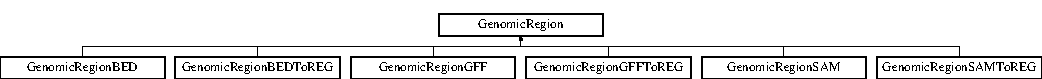
\includegraphics[height=1.06667cm]{classGenomicRegion}
\end{center}
\end{figure}
\subsection*{Public Member Functions}
\begin{CompactItemize}
\item 
\hypertarget{classGenomicRegion_8ff9fe5618b932a1caccbd9072ddaaef}{
\hyperlink{classGenomicRegion_8ff9fe5618b932a1caccbd9072ddaaef}{GenomicRegion} ()}
\label{classGenomicRegion_8ff9fe5618b932a1caccbd9072ddaaef}

\begin{CompactList}\small\item\em Empty class constructor. \item\end{CompactList}\item 
\hypertarget{classGenomicRegion_c45e11c7c0d0477c4b8682ef5266d3d7}{
\hyperlink{classGenomicRegion_c45e11c7c0d0477c4b8682ef5266d3d7}{GenomicRegion} (\hyperlink{classFileBuffer}{FileBuffer} $\ast$B)}
\label{classGenomicRegion_c45e11c7c0d0477c4b8682ef5266d3d7}

\begin{CompactList}\small\item\em Class constructor, see example below. \item\end{CompactList}\item 
\hypertarget{classGenomicRegion_c22559720502ea450aeb4f65c6c789e1}{
\hyperlink{classGenomicRegion_c22559720502ea450aeb4f65c6c789e1}{GenomicRegion} (char $\ast$inp, long int \hyperlink{classGenomicRegion_efe2255aeed5338060190ded05cb9c0c}{n\_\-line}=0)}
\label{classGenomicRegion_c22559720502ea450aeb4f65c6c789e1}

\begin{CompactList}\small\item\em Class constructor, see example below. \item\end{CompactList}\item 
\hypertarget{classGenomicRegion_6de3d0ff71615c36a7311509af56ae79}{
\hyperlink{classGenomicRegion_6de3d0ff71615c36a7311509af56ae79}{GenomicRegion} (char $\ast$label, \hyperlink{classGenomicInterval}{GenomicInterval} $\ast$i)}
\label{classGenomicRegion_6de3d0ff71615c36a7311509af56ae79}

\begin{CompactList}\small\item\em Class constructor. \item\end{CompactList}\item 
\hypertarget{classGenomicRegion_37af413ecbed6ee0d36ecbc40d957947}{
virtual \hyperlink{classGenomicRegion_37af413ecbed6ee0d36ecbc40d957947}{$\sim$GenomicRegion} ()}
\label{classGenomicRegion_37af413ecbed6ee0d36ecbc40d957947}

\begin{CompactList}\small\item\em Class destructor. \item\end{CompactList}\item 
\hypertarget{classGenomicRegion_fd188daab9b4e97ef66883d6971fe103}{
void \hyperlink{classGenomicRegion_fd188daab9b4e97ef66883d6971fe103}{Read} (char $\ast$inp, long int \hyperlink{classGenomicRegion_efe2255aeed5338060190ded05cb9c0c}{n\_\-line}=0, char del1=' ', char del2=',')}
\label{classGenomicRegion_fd188daab9b4e97ef66883d6971fe103}

\begin{CompactList}\small\item\em Reads label and genomic region intervals from input string {\bf inp}. \item\end{CompactList}\item 
\hypertarget{classGenomicRegion_40397d1fab7b00e5f04b9f7e52f0114e}{
virtual void \hyperlink{classGenomicRegion_40397d1fab7b00e5f04b9f7e52f0114e}{Print} (FILE $\ast$file\_\-ptr=stdout)}
\label{classGenomicRegion_40397d1fab7b00e5f04b9f7e52f0114e}

\begin{CompactList}\small\item\em Prints label and genomic region intervals with a newline character at the end. \item\end{CompactList}\item 
\hypertarget{classGenomicRegion_b9ea31af7fbb32f206efe0e64533a5be}{
virtual void \hyperlink{classGenomicRegion_b9ea31af7fbb32f206efe0e64533a5be}{PrintModified} (char $\ast$label, long int start, long int stop)}
\label{classGenomicRegion_b9ea31af7fbb32f206efe0e64533a5be}

\begin{CompactList}\small\item\em Same as \hyperlink{classGenomicRegion_40397d1fab7b00e5f04b9f7e52f0114e}{Print()}, but the label and interval's coordinates are modified. \item\end{CompactList}\item 
\hypertarget{classGenomicRegion_ba987d40590874eebd1dd8bb0c02bdc8}{
virtual void \hyperlink{classGenomicRegion_ba987d40590874eebd1dd8bb0c02bdc8}{PrintIntersection} (\hyperlink{classGenomicRegion}{GenomicRegion} $\ast$r, bool ignore\_\-strand, bool merge\_\-labels)}
\label{classGenomicRegion_ba987d40590874eebd1dd8bb0c02bdc8}

\begin{CompactList}\small\item\em Prints all pairwise intersection with the intervals in region {\bf r} (compatible, sorted and non-overlapping). \item\end{CompactList}\item 
\hypertarget{classGenomicRegion_cfe5347d9c92da801ce7e97416fc8758}{
virtual void \hyperlink{classGenomicRegion_cfe5347d9c92da801ce7e97416fc8758}{PrintConstrained} (\hyperlink{classGenomicRegion}{GenomicRegion} $\ast$r, bool merge\_\-labels=false)}
\label{classGenomicRegion_cfe5347d9c92da801ce7e97416fc8758}

\begin{CompactList}\small\item\em Same as \hyperlink{classGenomicRegion_40397d1fab7b00e5f04b9f7e52f0114e}{Print()}, but the interval is constrained between {\bf r-$>$I.front()-$>$START} and {\bf r-$>$I.back()-$>$STOP}. \item\end{CompactList}\item 
\hypertarget{classGenomicRegion_9c687565a8ed25da5a5ccf08e5e8461e}{
void \hyperlink{classGenomicRegion_9c687565a8ed25da5a5ccf08e5e8461e}{PrintREG} (bool compact=false)}
\label{classGenomicRegion_9c687565a8ed25da5a5ccf08e5e8461e}

\begin{CompactList}\small\item\em Prints label and genomic region intervals with a newline character at the end. \item\end{CompactList}\item 
\hypertarget{classGenomicRegion_9a00b031d4a119181b8b76ffa34a6f47}{
void \hyperlink{classGenomicRegion_9a00b031d4a119181b8b76ffa34a6f47}{PrintQ} (bool reverse=false)}
\label{classGenomicRegion_9a00b031d4a119181b8b76ffa34a6f47}

\begin{CompactList}\small\item\em Prints sequences (SEQ format). \item\end{CompactList}\item 
\hypertarget{classGenomicRegion_68ecc1c8c76e9204f6e27801f0ba3d5f}{
void \hyperlink{classGenomicRegion_68ecc1c8c76e9204f6e27801f0ba3d5f}{PrintError} (string error\_\-msg)}
\label{classGenomicRegion_68ecc1c8c76e9204f6e27801f0ba3d5f}

\begin{CompactList}\small\item\em Prints error message and exits. \item\end{CompactList}\item 
\hypertarget{classGenomicRegion_ad8566a736786134b72e7bf74296e807}{
void \hyperlink{classGenomicRegion_ad8566a736786134b72e7bf74296e807}{DeleteIntervals} (GenomicIntervalSet::iterator i, GenomicIntervalSet::iterator j)}
\label{classGenomicRegion_ad8566a736786134b72e7bf74296e807}

\begin{CompactList}\small\item\em Deletes intervals from iterator {\bf i} to {\bf j}. \item\end{CompactList}\item 
\hypertarget{classGenomicRegion_bc547e770917e859fa434d6c54954916}{
void \hyperlink{classGenomicRegion_bc547e770917e859fa434d6c54954916}{SetLabel} (char $\ast$label)}
\label{classGenomicRegion_bc547e770917e859fa434d6c54954916}

\begin{CompactList}\small\item\em Changes the label. \item\end{CompactList}\item 
\hypertarget{classGenomicRegion_e795532404bad8b93bec632c20d12b9d}{
void \hyperlink{classGenomicRegion_e795532404bad8b93bec632c20d12b9d}{SetStrand} (char strand)}
\label{classGenomicRegion_e795532404bad8b93bec632c20d12b9d}

\begin{CompactList}\small\item\em Interval strands are set to {\bf strand}. \item\end{CompactList}\item 
\hypertarget{classGenomicRegion_815baa00d7d33f179181560a1fe468fc}{
char $\ast$ \hyperlink{classGenomicRegion_815baa00d7d33f179181560a1fe468fc}{GetChromosome} ()}
\label{classGenomicRegion_815baa00d7d33f179181560a1fe468fc}

\begin{CompactList}\small\item\em Returns pointer to chromosome name. \item\end{CompactList}\item 
\hypertarget{classGenomicRegion_5bff7a3e83b0bc9bfb5441270d0ba1ae}{
size\_\-t \hyperlink{classGenomicRegion_5bff7a3e83b0bc9bfb5441270d0ba1ae}{GetSize} ()}
\label{classGenomicRegion_5bff7a3e83b0bc9bfb5441270d0ba1ae}

\begin{CompactList}\small\item\em Returns sum of interval's sizes. \item\end{CompactList}\item 
\hypertarget{classGenomicRegion_719143f1affa44c38493b2cd43448d3b}{
size\_\-t \hyperlink{classGenomicRegion_719143f1affa44c38493b2cd43448d3b}{GetSeqLength} (\hyperlink{classChromosomes}{Chromosomes} $\ast$C)}
\label{classGenomicRegion_719143f1affa44c38493b2cd43448d3b}

\begin{CompactList}\small\item\em Returns genomic region sequence length excluding 'N' characters. \item\end{CompactList}\item 
\hypertarget{classGenomicRegion_fcf7c053989b87f425f084d1f2c078f5}{
char $\ast$ \hyperlink{classGenomicRegion_fcf7c053989b87f425f084d1f2c078f5}{GetSeq} (\hyperlink{classChromosomes}{Chromosomes} $\ast$C, bool replace=false)}
\label{classGenomicRegion_fcf7c053989b87f425f084d1f2c078f5}

\begin{CompactList}\small\item\em Returns genomic region sequence. \item\end{CompactList}\item 
\hypertarget{classGenomicRegion_58c2fe162c1e9bbbd7c90d5abd011ff0}{
bool \hyperlink{classGenomicRegion_58c2fe162c1e9bbbd7c90d5abd011ff0}{IsCompatible} (bool ignore\_\-strand)}
\label{classGenomicRegion_58c2fe162c1e9bbbd7c90d5abd011ff0}

\begin{CompactList}\small\item\em Returns 'true' if all intervals are in the same chromosome and strand. \item\end{CompactList}\item 
\hypertarget{classGenomicRegion_2ebd984a2632314a39a6e9ba2c497105}{
bool \hyperlink{classGenomicRegion_2ebd984a2632314a39a6e9ba2c497105}{IsCompatibleWith} (\hyperlink{classGenomicRegion}{GenomicRegion} $\ast$r, bool ignore\_\-strand)}
\label{classGenomicRegion_2ebd984a2632314a39a6e9ba2c497105}

\begin{CompactList}\small\item\em Returns 'true' if all intervals are compatible with the intervals in {\bf r}. \item\end{CompactList}\item 
\hypertarget{classGenomicRegion_2e0765dfbe651ad583faa8c8a77e047f}{
bool \hyperlink{classGenomicRegion_2e0765dfbe651ad583faa8c8a77e047f}{IsCompatibleSorted} (bool ignore\_\-strand)}
\label{classGenomicRegion_2e0765dfbe651ad583faa8c8a77e047f}

\begin{CompactList}\small\item\em Returns 'true' if intervals are compatible and sorted by chromosome, strand (if {\bf ignore\_\-strand} is false) and start position. \item\end{CompactList}\item 
\hypertarget{classGenomicRegion_fb2db74a3cd85a84533375483e12b96c}{
bool \hyperlink{classGenomicRegion_fb2db74a3cd85a84533375483e12b96c}{IsCompatibleSortedAndNonoverlapping} ()}
\label{classGenomicRegion_fb2db74a3cd85a84533375483e12b96c}

\begin{CompactList}\small\item\em Returns 'true' if intervals are compatible, sorted and non-overlapping. \item\end{CompactList}\item 
\hypertarget{classGenomicRegion_9e3617a0046fe5fa8fce9f9cce8c3c37}{
bool \hyperlink{classGenomicRegion_9e3617a0046fe5fa8fce9f9cce8c3c37}{OverlapsWith} (\hyperlink{classGenomicRegion}{GenomicRegion} $\ast$r, bool ignore\_\-strand)}
\label{classGenomicRegion_9e3617a0046fe5fa8fce9f9cce8c3c37}

\begin{CompactList}\small\item\em Returns 'true' if it overlaps with input region {\bf r}. \item\end{CompactList}\item 
\hypertarget{classGenomicRegion_25634257eb7a2ed379548b17a83414fb}{
bool \hyperlink{classGenomicRegion_25634257eb7a2ed379548b17a83414fb}{IsBefore} (\hyperlink{classGenomicRegion}{GenomicRegion} $\ast$r, bool sorted\_\-by\_\-strand)}
\label{classGenomicRegion_25634257eb7a2ed379548b17a83414fb}

\begin{CompactList}\small\item\em Compares with input region {\bf r} and returns true if its order is before {\bf r}. The order is determined first by chromosome, second by strand, then by start position and finally by stop position. \item\end{CompactList}\item 
\hypertarget{classGenomicRegion_2065cf74a82c2340b1e49e7f7ec0fdd4}{
bool \hyperlink{classGenomicRegion_2065cf74a82c2340b1e49e7f7ec0fdd4}{IsPosBefore} (\hyperlink{classGenomicRegion}{GenomicRegion} $\ast$r)}
\label{classGenomicRegion_2065cf74a82c2340b1e49e7f7ec0fdd4}

\begin{CompactList}\small\item\em Compares with input region {\bf r} and returns true if its position order is before {\bf r}. The position order is determined first by start position and then by stop position. \item\end{CompactList}\item 
\hypertarget{classGenomicRegion_623e28aab180174d43873c4a85342ad4}{
long int \hyperlink{classGenomicRegion_623e28aab180174d43873c4a85342ad4}{CalcOverlap} (\hyperlink{classGenomicRegion}{GenomicRegion} $\ast$r, bool ignore\_\-strand)}
\label{classGenomicRegion_623e28aab180174d43873c4a85342ad4}

\begin{CompactList}\small\item\em Returns the total number of overlapping nucleotides (gaps are not matched) with input region {\bf r}. \item\end{CompactList}\item 
\hypertarget{classGenomicRegion_da548684fc4ae44dd3782aa15eaaf0a8}{
int \hyperlink{classGenomicRegion_da548684fc4ae44dd3782aa15eaaf0a8}{CalcDirection} (\hyperlink{classGenomicInterval}{GenomicInterval} $\ast$i, bool sorted\_\-by\_\-strand)}
\label{classGenomicRegion_da548684fc4ae44dd3782aa15eaaf0a8}

\begin{CompactList}\small\item\em Returns -1 if before interval {\bf i}, +1 if after, otherwise returns 0. The order is determined first by chromosome, then (optionally) by strand and finally by start position. \item\end{CompactList}\item 
\hypertarget{classGenomicRegion_b44366e44dc9a83da65b9593ce90dd32}{
int \hyperlink{classGenomicRegion_b44366e44dc9a83da65b9593ce90dd32}{CalcDirection} (\hyperlink{classGenomicRegion}{GenomicRegion} $\ast$r, bool sorted\_\-by\_\-strand)}
\label{classGenomicRegion_b44366e44dc9a83da65b9593ce90dd32}

\begin{CompactList}\small\item\em Returns -1 if before region {\bf r}, +1 if after, otherwise returns 0. The order is determined first by chromosome, then (optionally) by strand and finally by start position. \item\end{CompactList}\item 
\hypertarget{classGenomicRegion_90b0382a60f0a8532af73fc18f41364b}{
virtual void \hyperlink{classGenomicRegion_90b0382a60f0a8532af73fc18f41364b}{RunAlign} (\hyperlink{classChromosomes}{Chromosomes} $\ast$C)}
\label{classGenomicRegion_90b0382a60f0a8532af73fc18f41364b}

\begin{CompactList}\small\item\em Prints alignments of input sequences to reference genome. \item\end{CompactList}\item 
\hypertarget{classGenomicRegion_405010d9256a3c08c53adee98133cb62}{
virtual void \hyperlink{classGenomicRegion_405010d9256a3c08c53adee98133cb62}{PrintBEDFormat} (char $\ast$color, bool convert\_\-chromosome)}
\label{classGenomicRegion_405010d9256a3c08c53adee98133cb62}

\begin{CompactList}\small\item\em Prints in BED format. If {\bf convert\_\-chromosome} is 'true', then convert from ENSEMBL to UCSC names (by adding 'chr' prefix to each chromosome name, and by converting 'MT' to 'chrM'). \item\end{CompactList}\item 
\hypertarget{classGenomicRegion_11b494e59775ac255ddb469c98f8a8a8}{
virtual bool \hyperlink{classGenomicRegion_11b494e59775ac255ddb469c98f8a8a8}{ApplyBounds} (StringLIntMap $\ast$bounds)}
\label{classGenomicRegion_11b494e59775ac255ddb469c98f8a8a8}

\begin{CompactList}\small\item\em Corrects interval start/stop positions so as to comply with chromosomal bounds. \item\end{CompactList}\item 
\hypertarget{classGenomicRegion_1e9a85a086afbe2608411450c9a4c5e6}{
virtual void \hyperlink{classGenomicRegion_1e9a85a086afbe2608411450c9a4c5e6}{Center} ()}
\label{classGenomicRegion_1e9a85a086afbe2608411450c9a4c5e6}

\begin{CompactList}\small\item\em Replace each interval in the region with the corresponding center interval. \item\end{CompactList}\item 
\hypertarget{classGenomicRegion_c2c426782bd7c0d302b7a77bb1ff047f}{
virtual void \hyperlink{classGenomicRegion_c2c426782bd7c0d302b7a77bb1ff047f}{Connect} ()}
\label{classGenomicRegion_c2c426782bd7c0d302b7a77bb1ff047f}

\begin{CompactList}\small\item\em Replace region with a single interval from minimum start to maximum stop position. \item\end{CompactList}\item 
\hypertarget{classGenomicRegion_869de97ecf059355fe5a5b572b5c2575}{
virtual void \hyperlink{classGenomicRegion_869de97ecf059355fe5a5b572b5c2575}{Diff} ()}
\label{classGenomicRegion_869de97ecf059355fe5a5b572b5c2575}

\begin{CompactList}\small\item\em Replace regions with the corresponding gap intervals between successive intervals (e.g. used to compute intron boundaries). \item\end{CompactList}\item 
\hypertarget{classGenomicRegion_98695d5d1056d693a1c635b197f4b8bf}{
virtual void \hyperlink{classGenomicRegion_98695d5d1056d693a1c635b197f4b8bf}{RunCalcDistances} (char $\ast$op1, char $\ast$op2)}
\label{classGenomicRegion_98695d5d1056d693a1c635b197f4b8bf}

\begin{CompactList}\small\item\em Print distance between successive intervals. \item\end{CompactList}\item 
\hypertarget{classGenomicRegion_0785438db56d7b7cc7539470e85434dd}{
virtual void \hyperlink{classGenomicRegion_0785438db56d7b7cc7539470e85434dd}{Divide} ()}
\label{classGenomicRegion_0785438db56d7b7cc7539470e85434dd}

\begin{CompactList}\small\item\em Divide intervals divided in half (i.e. two intervals for each original interval in the genomic region). \item\end{CompactList}\item 
\hypertarget{classGenomicRegion_45fe5d619f2e21644eacb6984aa47eff}{
virtual void \hyperlink{classGenomicRegion_45fe5d619f2e21644eacb6984aa47eff}{RunDivide} ()}
\label{classGenomicRegion_45fe5d619f2e21644eacb6984aa47eff}

\begin{CompactList}\small\item\em Print intervals divided in half (i.e. two intervals for each original interval in the genomic region). \item\end{CompactList}\item 
\hypertarget{classGenomicRegion_048d2182b212789b182c2c82a7ac131e}{
virtual void \hyperlink{classGenomicRegion_048d2182b212789b182c2c82a7ac131e}{Fix} ()}
\label{classGenomicRegion_048d2182b212789b182c2c82a7ac131e}

\begin{CompactList}\small\item\em Removes rogue intervals (e.g. start$>$stop). \item\end{CompactList}\item 
\hypertarget{classGenomicRegion_8075e77ab6296b59506857cc21ee4c9d}{
virtual void \hyperlink{classGenomicRegion_8075e77ab6296b59506857cc21ee4c9d}{Intersect} ()}
\label{classGenomicRegion_8075e77ab6296b59506857cc21ee4c9d}

\begin{CompactList}\small\item\em Print intersection among all intervals, i.e. maximum start to minimum stop position. \item\end{CompactList}\item 
\hypertarget{classGenomicRegion_08db190bc63e6f1d6fc90679dc5e6868}{
void \hyperlink{classGenomicRegion_08db190bc63e6f1d6fc90679dc5e6868}{RunSize} ()}
\label{classGenomicRegion_08db190bc63e6f1d6fc90679dc5e6868}

\begin{CompactList}\small\item\em Prints region label and sum of intervals' sizes. \item\end{CompactList}\item 
virtual void \hyperlink{classGenomicRegion_0721b07af0850057e4ab9cd416ecac2f}{ModifyPos} (char $\ast$position\_\-op, long int position\_\-shift)
\begin{CompactList}\small\item\em Modifies interval start/stop positions. First it chooses which position to keep fixed, and then it shifts the non-fixed position. \item\end{CompactList}\item 
\hypertarget{classGenomicRegion_222b3b8f567c306ee5a71ea3a720ef43}{
virtual void \hyperlink{classGenomicRegion_222b3b8f567c306ee5a71ea3a720ef43}{Randomize} (gsl\_\-rng $\ast$random\_\-generator, StringLIntMap $\ast$bounds)}
\label{classGenomicRegion_222b3b8f567c306ee5a71ea3a720ef43}

\begin{CompactList}\small\item\em Randomizes interval position within chromosomal bounds. \item\end{CompactList}\item 
\hypertarget{classGenomicRegion_6120af435fb9ee68cb5a3d5066a4fda4}{
void \hyperlink{classGenomicRegion_6120af435fb9ee68cb5a3d5066a4fda4}{ReversePos} (StringLIntMap $\ast$bounds)}
\label{classGenomicRegion_6120af435fb9ee68cb5a3d5066a4fda4}

\begin{CompactList}\small\item\em Reverses interval start/stop positions with respect to chromosomal bounds, as if the reference point were in the end of the chromosome as opposed to the beginning. \item\end{CompactList}\item 
\hypertarget{classGenomicRegion_461fbb00db1b45061e641f37614fb146}{
virtual void \hyperlink{classGenomicRegion_461fbb00db1b45061e641f37614fb146}{Select} (bool first, bool last, bool from5p, bool from3p)}
\label{classGenomicRegion_461fbb00db1b45061e641f37614fb146}

\begin{CompactList}\small\item\em Selects a subset of intervals according to their relative positions. \item\end{CompactList}\item 
virtual void \hyperlink{classGenomicRegion_0ee8c165839c79afdc586f8b5e07788e}{ShiftPos} (long int start\_\-shift, long int stop\_\-shift, bool strand\_\-aware)
\begin{CompactList}\small\item\em Shifts interval start/stop positions. First it chooses reference position, and then shifts start and stop positions separately. \item\end{CompactList}\item 
\hypertarget{classGenomicRegion_b2c52ae40b34f3607f4558add94c25fd}{
virtual void \hyperlink{classGenomicRegion_b2c52ae40b34f3607f4558add94c25fd}{RunShuffle} (gsl\_\-rng $\ast$random\_\-generator, \hyperlink{classGenomicRegionSet}{GenomicRegionSet} $\ast$refReg, StringLIntMap $\ast$index, StringVecLIntMap $\ast$loc)}
\label{classGenomicRegion_b2c52ae40b34f3607f4558add94c25fd}

\begin{CompactList}\small\item\em Prints shuffled region within specified reference regions in {\bf refReg}. \item\end{CompactList}\item 
\hypertarget{classGenomicRegion_03959dc5b5695d817b5a40b47f30a4aa}{
virtual void \hyperlink{classGenomicRegion_03959dc5b5695d817b5a40b47f30a4aa}{Sort} ()}
\label{classGenomicRegion_03959dc5b5695d817b5a40b47f30a4aa}

\begin{CompactList}\small\item\em Sort intervals according to start position (only for compatible intervals). \item\end{CompactList}\item 
\hypertarget{classGenomicRegion_1686d4f4d2962b22d506a25a5887c31c}{
virtual void \hyperlink{classGenomicRegion_1686d4f4d2962b22d506a25a5887c31c}{RunSplit} ()}
\label{classGenomicRegion_1686d4f4d2962b22d506a25a5887c31c}

\begin{CompactList}\small\item\em Print region intervals on separate lines. \item\end{CompactList}\item 
\hypertarget{classGenomicRegion_e19cd6eaa883e6517ba12567cd756320}{
virtual void \hyperlink{classGenomicRegion_e19cd6eaa883e6517ba12567cd756320}{ModifyStrand} (char $\ast$strand\_\-op)}
\label{classGenomicRegion_e19cd6eaa883e6517ba12567cd756320}

\begin{CompactList}\small\item\em Modified strand information: '+'=only forward, '-'=only reverse, 'r'=reverse strands from '+' to '-' and vice versa, 'b'=both strands. \item\end{CompactList}\item 
\hypertarget{classGenomicRegion_05cb47d38946b780f7eb585074ccf393}{
virtual void \hyperlink{classGenomicRegion_05cb47d38946b780f7eb585074ccf393}{Union} ()}
\label{classGenomicRegion_05cb47d38946b780f7eb585074ccf393}

\begin{CompactList}\small\item\em Compute intervals' union. \item\end{CompactList}\item 
\hypertarget{classGenomicRegion_3d90c15accabfd5c0279f27f3513ba7c}{
virtual void \hyperlink{classGenomicRegion_3d90c15accabfd5c0279f27f3513ba7c}{RunUnion} ()}
\label{classGenomicRegion_3d90c15accabfd5c0279f27f3513ba7c}

\begin{CompactList}\small\item\em Print intervals' union. \item\end{CompactList}\item 
\hypertarget{classGenomicRegion_3962ea71432f3977b1ac501e4e878480}{
virtual void \hyperlink{classGenomicRegion_3962ea71432f3977b1ac501e4e878480}{PrintWindows} (long int win\_\-step, long int win\_\-size)}
\label{classGenomicRegion_3962ea71432f3977b1ac501e4e878480}

\begin{CompactList}\small\item\em Print sliding windows (implemented only for single-interval regions). \item\end{CompactList}\item 
\hypertarget{classGenomicRegion_a2a5b753401e9f9d64a30cfbbdf23f60}{
void \hyperlink{classGenomicRegion_a2a5b753401e9f9d64a30cfbbdf23f60}{PrintRemoveN} (\hyperlink{classChromosomes}{Chromosomes} $\ast$C)}
\label{classGenomicRegion_a2a5b753401e9f9d64a30cfbbdf23f60}

\begin{CompactList}\small\item\em Remove sub-intervals that correspond to sequences of 'N' characters. \item\end{CompactList}\item 
\hypertarget{classGenomicRegion_4b52d78052e0109b1fceafe450cfdedd}{
void \hyperlink{classGenomicRegion_4b52d78052e0109b1fceafe450cfdedd}{PrintSeq} (\hyperlink{classChromosomes}{Chromosomes} $\ast$C, bool replace=false)}
\label{classGenomicRegion_4b52d78052e0109b1fceafe450cfdedd}

\begin{CompactList}\small\item\em Prints region label, intervals and extracted sequence in SEQ format. \item\end{CompactList}\item 
void \hyperlink{classGenomicRegion_33d1e5544b3fb81e8c19468b91920b1d}{PrintOffsetFormat} (char $\ast$op, bool fraction)
\begin{CompactList}\small\item\em Calculates the offset distances of interval start and stop position with respect to the first interval in the set. \item\end{CompactList}\item 
\hypertarget{classGenomicRegion_7a8ac4f469447256253bdbdcb1b4a956}{
void \hyperlink{classGenomicRegion_7a8ac4f469447256253bdbdcb1b4a956}{PrintSeqLength} (\hyperlink{classChromosomes}{Chromosomes} $\ast$C)}
\label{classGenomicRegion_7a8ac4f469447256253bdbdcb1b4a956}

\begin{CompactList}\small\item\em Prints region label and sequence length (excluding 'N' characters). \item\end{CompactList}\item 
\hypertarget{classGenomicRegion_77fa696d55d538b365d15a7a30391132}{
void \hyperlink{classGenomicRegion_77fa696d55d538b365d15a7a30391132}{PrintVerifySeq} (\hyperlink{classChromosomes}{Chromosomes} $\ast$C, bool ignore)}
\label{classGenomicRegion_77fa696d55d538b365d15a7a30391132}

\begin{CompactList}\small\item\em Verifies extracted sequence against region label. \item\end{CompactList}\item 
\hypertarget{classGenomicRegion_9304039f70c5110b961cc9de77974d09}{
void \hyperlink{classGenomicRegion_9304039f70c5110b961cc9de77974d09}{ReverseStrand} ()}
\label{classGenomicRegion_9304039f70c5110b961cc9de77974d09}

\begin{CompactList}\small\item\em If interval strand is '+', it is changed to '-' and vice versa. \item\end{CompactList}\item 
\hypertarget{classGenomicRegion_50f5ba99404da1cdae6a8632a19ff837}{
\hyperlink{classGenomicRegion}{GenomicRegion} $\ast$ \hyperlink{classGenomicRegion_50f5ba99404da1cdae6a8632a19ff837}{Constrain} (\hyperlink{classGenomicRegion}{GenomicRegion} $\ast$r, char $\ast$label=NULL)}
\label{classGenomicRegion_50f5ba99404da1cdae6a8632a19ff837}

\begin{CompactList}\small\item\em Returns a version of this genomic region constrained by the start/stop coordinates. \item\end{CompactList}\item 
\hypertarget{classGenomicRegion_44cf789afda4e77749019045050e5ec7}{
virtual \hyperlink{classGenomicRegion}{GenomicRegion} $\ast$ \hyperlink{classGenomicRegion_44cf789afda4e77749019045050e5ec7}{Diff} (\hyperlink{classGenomicRegion}{GenomicRegion} $\ast$r)}
\label{classGenomicRegion_44cf789afda4e77749019045050e5ec7}

\begin{CompactList}\small\item\em Returns the difference of this genomic region and region {\bf r}. \item\end{CompactList}\end{CompactItemize}
\subsection*{Public Attributes}
\begin{CompactItemize}
\item 
\hypertarget{classGenomicRegion_efe2255aeed5338060190ded05cb9c0c}{
unsigned long int \hyperlink{classGenomicRegion_efe2255aeed5338060190ded05cb9c0c}{n\_\-line}}
\label{classGenomicRegion_efe2255aeed5338060190ded05cb9c0c}

\begin{CompactList}\small\item\em keeps track of line number \item\end{CompactList}\item 
\hypertarget{classGenomicRegion_7eeba95c1e87e100346688681e30ff24}{
char $\ast$ \hyperlink{classGenomicRegion_7eeba95c1e87e100346688681e30ff24}{LABEL}}
\label{classGenomicRegion_7eeba95c1e87e100346688681e30ff24}

\begin{CompactList}\small\item\em genomic region label \item\end{CompactList}\item 
\hypertarget{classGenomicRegion_b10b86b03c258958818b00c21e3672a9}{
GenomicIntervalSet \hyperlink{classGenomicRegion_b10b86b03c258958818b00c21e3672a9}{I}}
\label{classGenomicRegion_b10b86b03c258958818b00c21e3672a9}

\begin{CompactList}\small\item\em set of intervals \item\end{CompactList}\end{CompactItemize}


\subsection{Detailed Description}
This class implements the genomic regions (i.e. ordered sets of genomic intervals). 

Example: 

\begin{Code}\begin{verbatim}    GenomicRegionREG x("Region#1\tchr1 + 132034 135932 chr1 + 135832 140102");          // standard REG format
    GenomicRegionREG y("Region#2\tchr1 + 132034,135832 135932,140102");                         // compact REG format
    cout << "x = \n"; x.Print();
    cout << "y = \n"; y.Print(); 
\end{verbatim}
\end{Code}

 

\subsection{Member Function Documentation}
\hypertarget{classGenomicRegion_0721b07af0850057e4ab9cd416ecac2f}{
\index{GenomicRegion@{GenomicRegion}!ModifyPos@{ModifyPos}}
\index{ModifyPos@{ModifyPos}!GenomicRegion@{GenomicRegion}}
\subsubsection[ModifyPos]{\setlength{\rightskip}{0pt plus 5cm}void GenomicRegion::ModifyPos (char $\ast$ {\em position\_\-op}, \/  long int {\em position\_\-shift})\hspace{0.3cm}{\tt  \mbox{[}virtual\mbox{]}}}}
\label{classGenomicRegion_0721b07af0850057e4ab9cd416ecac2f}


Modifies interval start/stop positions. First it chooses which position to keep fixed, and then it shifts the non-fixed position. 

\begin{Desc}
\item[Parameters:]
\begin{description}
\item[{\em position\_\-op}]selects fixed position as follows: '1'=start position, 'c'=center position, '5p'=5-prime, '3p'=3-prime \item[{\em position\_\-shift}]determines the shift of the non-fixed position (in the 'c' case, both positions are shifted symmetrically around the center) \end{description}
\end{Desc}


Reimplemented in \hyperlink{classGenomicRegionBED_c515c70f443db400f911452ed359433b}{GenomicRegionBED}, and \hyperlink{classGenomicRegionSAM_353207352073db00dee0a9b620dca197}{GenomicRegionSAM}.\hypertarget{classGenomicRegion_0ee8c165839c79afdc586f8b5e07788e}{
\index{GenomicRegion@{GenomicRegion}!ShiftPos@{ShiftPos}}
\index{ShiftPos@{ShiftPos}!GenomicRegion@{GenomicRegion}}
\subsubsection[ShiftPos]{\setlength{\rightskip}{0pt plus 5cm}void GenomicRegion::ShiftPos (long int {\em start\_\-shift}, \/  long int {\em stop\_\-shift}, \/  bool {\em strand\_\-aware})\hspace{0.3cm}{\tt  \mbox{[}virtual\mbox{]}}}}
\label{classGenomicRegion_0ee8c165839c79afdc586f8b5e07788e}


Shifts interval start/stop positions. First it chooses reference position, and then shifts start and stop positions separately. 

\begin{Desc}
\item[Parameters:]
\begin{description}
\item[{\em start\_\-shift}]determines the shift of the start position \item[{\em stop\_\-shift}]determines the shift of the stop position \item[{\em strand\_\-aware}]if 'true', then start=5-prime and stop=3-prime \end{description}
\end{Desc}


Reimplemented in \hyperlink{classGenomicRegionBED_fd2f05cec2af5186794f40f221e040b1}{GenomicRegionBED}, and \hyperlink{classGenomicRegionSAM_fb2701ba1a521ae2c07ea0ace2f9ee77}{GenomicRegionSAM}.\hypertarget{classGenomicRegion_33d1e5544b3fb81e8c19468b91920b1d}{
\index{GenomicRegion@{GenomicRegion}!PrintOffsetFormat@{PrintOffsetFormat}}
\index{PrintOffsetFormat@{PrintOffsetFormat}!GenomicRegion@{GenomicRegion}}
\subsubsection[PrintOffsetFormat]{\setlength{\rightskip}{0pt plus 5cm}void GenomicRegion::PrintOffsetFormat (char $\ast$ {\em op}, \/  bool {\em fraction})}}
\label{classGenomicRegion_33d1e5544b3fb81e8c19468b91920b1d}


Calculates the offset distances of interval start and stop position with respect to the first interval in the set. 

\begin{Desc}
\item[Parameters:]
\begin{description}
\item[{\em op}]determines reference point as follows: '1'=start position, '2'=stop position, '5p'=5-prime position, '3p'=3-prime position \item[{\em fraction}]if 'true', offsets are reported as a fraction of the total region length \end{description}
\end{Desc}


The documentation for this class was generated from the following files:\begin{CompactItemize}
\item 
genomic\_\-intervals.h\item 
genomic\_\-intervals.cpp\end{CompactItemize}

\hypertarget{classGenomicRegionBED}{
\section{GenomicRegionBED Class Reference}
\label{classGenomicRegionBED}\index{GenomicRegionBED@{GenomicRegionBED}}
}
This class processes genomic regions in BED format.  


{\tt \#include $<$genomic\_\-intervals.h$>$}

Inheritance diagram for GenomicRegionBED::\begin{figure}[H]
\begin{center}
\leavevmode
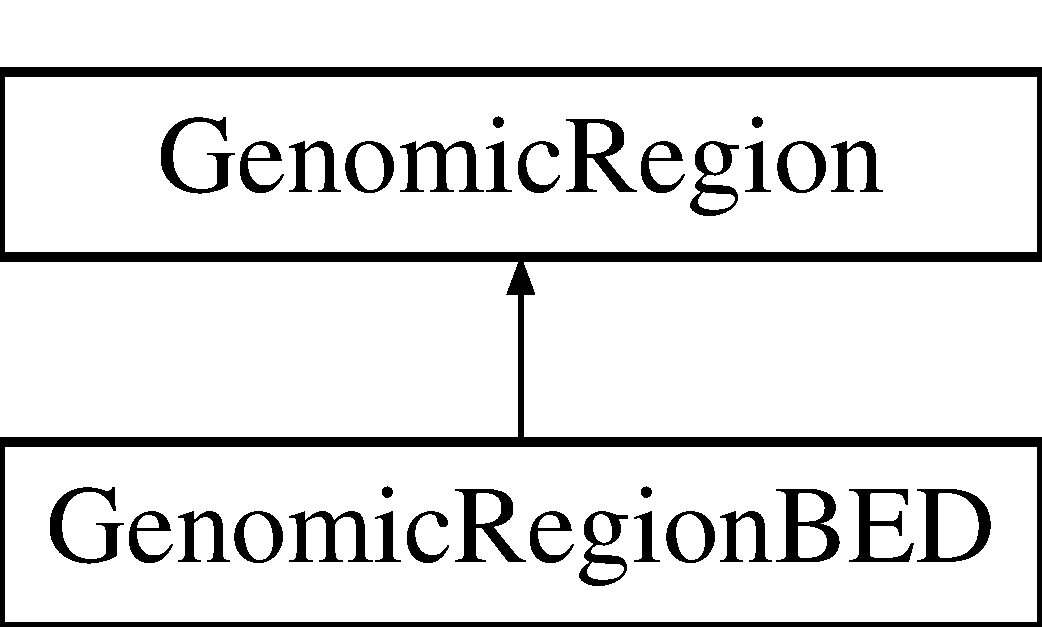
\includegraphics[height=2cm]{classGenomicRegionBED}
\end{center}
\end{figure}
\subsection*{Public Member Functions}
\begin{CompactItemize}
\item 
\hypertarget{classGenomicRegionBED_89d54edc5809d113202c9f09f82e1057}{
\hyperlink{classGenomicRegionBED_89d54edc5809d113202c9f09f82e1057}{GenomicRegionBED} (\hyperlink{classFileBuffer}{FileBuffer} $\ast$B)}
\label{classGenomicRegionBED_89d54edc5809d113202c9f09f82e1057}

\begin{CompactList}\small\item\em Class constructor, see example below. \item\end{CompactList}\item 
\hypertarget{classGenomicRegionBED_4d7c87327c1074258ac1e6b5ac87c9dd}{
\hyperlink{classGenomicRegionBED_4d7c87327c1074258ac1e6b5ac87c9dd}{GenomicRegionBED} (char $\ast$inp, long int \hyperlink{classGenomicRegion_efe2255aeed5338060190ded05cb9c0c}{n\_\-line}=0)}
\label{classGenomicRegionBED_4d7c87327c1074258ac1e6b5ac87c9dd}

\begin{CompactList}\small\item\em Class constructor, see example below. \item\end{CompactList}\item 
\hypertarget{classGenomicRegionBED_a6e68da10b635bcd84bf320b94a4d414}{
\hyperlink{classGenomicRegionBED_a6e68da10b635bcd84bf320b94a4d414}{GenomicRegionBED} (char $\ast$label, \hyperlink{classGenomicInterval}{GenomicInterval} $\ast$i)}
\label{classGenomicRegionBED_a6e68da10b635bcd84bf320b94a4d414}

\begin{CompactList}\small\item\em Class constructor. \item\end{CompactList}\item 
\hypertarget{classGenomicRegionBED_a27241b7fbdb90e0b4b1e411045d080f}{
\hyperlink{classGenomicRegionBED_a27241b7fbdb90e0b4b1e411045d080f}{$\sim$GenomicRegionBED} ()}
\label{classGenomicRegionBED_a27241b7fbdb90e0b4b1e411045d080f}

\begin{CompactList}\small\item\em Class destructor. \item\end{CompactList}\item 
\hypertarget{classGenomicRegionBED_707a1744e040214d78d37b928f1f0252}{
void \hyperlink{classGenomicRegionBED_707a1744e040214d78d37b928f1f0252}{Read} (char $\ast$inp, long int \hyperlink{classGenomicRegion_efe2255aeed5338060190ded05cb9c0c}{n\_\-line}=0)}
\label{classGenomicRegionBED_707a1744e040214d78d37b928f1f0252}

\begin{CompactList}\small\item\em Reads BED format from input string {\bf inp}. \item\end{CompactList}\item 
\hypertarget{classGenomicRegionBED_ffbd8eb279f10f9b45189e2388fe7e89}{
void \hyperlink{classGenomicRegionBED_ffbd8eb279f10f9b45189e2388fe7e89}{Print} (FILE $\ast$file\_\-ptr=stdout)}
\label{classGenomicRegionBED_ffbd8eb279f10f9b45189e2388fe7e89}

\begin{CompactList}\small\item\em Prints label and genomic region intervals with a newline character at the end. \item\end{CompactList}\item 
\hypertarget{classGenomicRegionBED_e194ce2d67eafe222f10172ee376de94}{
void \hyperlink{classGenomicRegionBED_e194ce2d67eafe222f10172ee376de94}{Print} (FILE $\ast$file\_\-ptr, char $\ast$color, bool convert\_\-chromosome)}
\label{classGenomicRegionBED_e194ce2d67eafe222f10172ee376de94}

\begin{CompactList}\small\item\em Same as generic \hyperlink{classGenomicRegionBED_ffbd8eb279f10f9b45189e2388fe7e89}{Print()} except that it modifies the color and the chromosome names. \item\end{CompactList}\item 
\hypertarget{classGenomicRegionBED_04eceeb473bee498747bdd68d8ba8806}{
void \hyperlink{classGenomicRegionBED_04eceeb473bee498747bdd68d8ba8806}{PrintIntersection} (\hyperlink{classGenomicRegion}{GenomicRegion} $\ast$r, bool ignore\_\-strand, bool merge\_\-labels)}
\label{classGenomicRegionBED_04eceeb473bee498747bdd68d8ba8806}

\begin{CompactList}\small\item\em Prints all pairwise intersection with the intervals in region {\bf r} (compatible, sorted and non-overlapping). \item\end{CompactList}\item 
\hypertarget{classGenomicRegionBED_25a8584259b6a8d47aa8c46795de1880}{
void \hyperlink{classGenomicRegionBED_25a8584259b6a8d47aa8c46795de1880}{PrintConstrained} (\hyperlink{classGenomicRegion}{GenomicRegion} $\ast$r, bool merge\_\-labels=false)}
\label{classGenomicRegionBED_25a8584259b6a8d47aa8c46795de1880}

\begin{CompactList}\small\item\em Same as \hyperlink{classGenomicRegionBED_ffbd8eb279f10f9b45189e2388fe7e89}{Print()}, but the interval is constrained between {\bf start} and {\bf stop}. \item\end{CompactList}\item 
\hypertarget{classGenomicRegionBED_aebba3c31c0fa88e594706f490030549}{
void \hyperlink{classGenomicRegionBED_aebba3c31c0fa88e594706f490030549}{PrintModified} (char $\ast$label, long int start, long int stop)}
\label{classGenomicRegionBED_aebba3c31c0fa88e594706f490030549}

\begin{CompactList}\small\item\em Same as \hyperlink{classGenomicRegionBED_ffbd8eb279f10f9b45189e2388fe7e89}{Print()}, but the label and interval's coordinates are modified. \item\end{CompactList}\item 
\hypertarget{classGenomicRegionBED_01bd886cfa67a3adae10c67dee941924}{
void \hyperlink{classGenomicRegionBED_01bd886cfa67a3adae10c67dee941924}{UpdateThick} ()}
\label{classGenomicRegionBED_01bd886cfa67a3adae10c67dee941924}

\begin{CompactList}\small\item\em Auxiliary function: updates thickStart/thickEnd variables to honor changes in coordinates. \item\end{CompactList}\item 
\hypertarget{classGenomicRegionBED_513fb071e2626be58837052daf86bab5}{
void \hyperlink{classGenomicRegionBED_513fb071e2626be58837052daf86bab5}{PrintBEDFormat} (char $\ast$color, bool convert\_\-chromosome)}
\label{classGenomicRegionBED_513fb071e2626be58837052daf86bab5}

\begin{CompactList}\small\item\em Prints in BED format. If {\bf convert\_\-chromosome} is 'true', then convert from ENSEMBL to UCSC names (by adding 'chr' prefix to each chromosome name, and by converting 'MT' to 'chrM'). \item\end{CompactList}\item 
\hypertarget{classGenomicRegionBED_5056b98f57933e2d24fd6d601f5499ef}{
void \hyperlink{classGenomicRegionBED_5056b98f57933e2d24fd6d601f5499ef}{ApplyBounds} (StringLIntMap $\ast$bounds)}
\label{classGenomicRegionBED_5056b98f57933e2d24fd6d601f5499ef}

\begin{CompactList}\small\item\em Corrects interval start/stop positions so as to comply with chromosomal bounds. \item\end{CompactList}\item 
\hypertarget{classGenomicRegionBED_35c692c1343327d9cb450cfa1276096f}{
void \hyperlink{classGenomicRegionBED_35c692c1343327d9cb450cfa1276096f}{Center} ()}
\label{classGenomicRegionBED_35c692c1343327d9cb450cfa1276096f}

\begin{CompactList}\small\item\em Replace each interval in the region with the corresponding center interval. \item\end{CompactList}\item 
\hypertarget{classGenomicRegionBED_d55a9ffea8b0924bac3d11a5722cdfd2}{
void \hyperlink{classGenomicRegionBED_d55a9ffea8b0924bac3d11a5722cdfd2}{Connect} ()}
\label{classGenomicRegionBED_d55a9ffea8b0924bac3d11a5722cdfd2}

\begin{CompactList}\small\item\em Replace region with a single interval from minimum start to maximum stop position. \item\end{CompactList}\item 
\hypertarget{classGenomicRegionBED_9580179a120834e71ac90e56e5f35aa9}{
void \hyperlink{classGenomicRegionBED_9580179a120834e71ac90e56e5f35aa9}{Diff} ()}
\label{classGenomicRegionBED_9580179a120834e71ac90e56e5f35aa9}

\begin{CompactList}\small\item\em Replace regions with the corresponding gap intervals between successive intervals (e.g. used to compute intron boundaries). \item\end{CompactList}\item 
\hypertarget{classGenomicRegionBED_833d50369e61f64603c63b6a05f3d80b}{
void \hyperlink{classGenomicRegionBED_833d50369e61f64603c63b6a05f3d80b}{RunCalcDistances} (char $\ast$op1, char $\ast$op2)}
\label{classGenomicRegionBED_833d50369e61f64603c63b6a05f3d80b}

\begin{CompactList}\small\item\em Print distance between successive intervals. \item\end{CompactList}\item 
\hypertarget{classGenomicRegionBED_be056ec84d2d6890479d47559839bab4}{
void \hyperlink{classGenomicRegionBED_be056ec84d2d6890479d47559839bab4}{Divide} ()}
\label{classGenomicRegionBED_be056ec84d2d6890479d47559839bab4}

\begin{CompactList}\small\item\em Divide intervals divided in half (i.e. two intervals for each original interval in the genomic region). \item\end{CompactList}\item 
\hypertarget{classGenomicRegionBED_5f456b4af154c98968370568828d6e3d}{
void \hyperlink{classGenomicRegionBED_5f456b4af154c98968370568828d6e3d}{RunDivide} ()}
\label{classGenomicRegionBED_5f456b4af154c98968370568828d6e3d}

\begin{CompactList}\small\item\em Print intervals divided in half (i.e. two intervals for each original interval in the genomic region). \item\end{CompactList}\item 
\hypertarget{classGenomicRegionBED_ac069dcf513265f7756b72c106f2765c}{
void \hyperlink{classGenomicRegionBED_ac069dcf513265f7756b72c106f2765c}{Fix} ()}
\label{classGenomicRegionBED_ac069dcf513265f7756b72c106f2765c}

\begin{CompactList}\small\item\em Removes rogue intervals (e.g. start$>$stop). \item\end{CompactList}\item 
\hypertarget{classGenomicRegionBED_cf815a65712e82bf3f8c596c795f55c4}{
void \hyperlink{classGenomicRegionBED_cf815a65712e82bf3f8c596c795f55c4}{Intersect} ()}
\label{classGenomicRegionBED_cf815a65712e82bf3f8c596c795f55c4}

\begin{CompactList}\small\item\em Print intersection among all intervals, i.e. maximum start to minimum stop position. \item\end{CompactList}\item 
void \hyperlink{classGenomicRegionBED_c515c70f443db400f911452ed359433b}{ModifyPos} (char $\ast$position\_\-op, long int position\_\-shift)
\begin{CompactList}\small\item\em Modifies interval start/stop positions. First it chooses which position to keep fixed, and then it shifts the non-fixed position. \item\end{CompactList}\item 
\hypertarget{classGenomicRegionBED_920d47deb095506c311da2b2324e7a14}{
void \hyperlink{classGenomicRegionBED_920d47deb095506c311da2b2324e7a14}{Randomize} (gsl\_\-rng $\ast$random\_\-generator, StringLIntMap $\ast$bounds)}
\label{classGenomicRegionBED_920d47deb095506c311da2b2324e7a14}

\begin{CompactList}\small\item\em Randomizes interval position within chromosomal bounds. \item\end{CompactList}\item 
\hypertarget{classGenomicRegionBED_dec7408315765bbdb21465a26400422b}{
void \hyperlink{classGenomicRegionBED_dec7408315765bbdb21465a26400422b}{Select} (bool first, bool last, bool from5p, bool from3p)}
\label{classGenomicRegionBED_dec7408315765bbdb21465a26400422b}

\begin{CompactList}\small\item\em Selects a subset of intervals according to their relative positions. \item\end{CompactList}\item 
void \hyperlink{classGenomicRegionBED_97d00cb29eb1f379b9e6ee17197530c7}{ShiftPos} (long int start\_\-shift, long int stop\_\-shift, bool shift\_\-5prime)
\begin{CompactList}\small\item\em Shifts interval start/stop positions. First it chooses reference position, and then shifts start and stop positions separately. \item\end{CompactList}\item 
\hypertarget{classGenomicRegionBED_f3793387aa335bf68042f9245bc5992d}{
void \hyperlink{classGenomicRegionBED_f3793387aa335bf68042f9245bc5992d}{RunShuffle} (gsl\_\-rng $\ast$random\_\-generator, \hyperlink{classGenomicRegionSet}{GenomicRegionSet} $\ast$refReg, StringLIntMap $\ast$index, StringVecLIntMap $\ast$loc)}
\label{classGenomicRegionBED_f3793387aa335bf68042f9245bc5992d}

\begin{CompactList}\small\item\em Prints shuffled region within specified reference regions in {\bf refReg}. \item\end{CompactList}\item 
\hypertarget{classGenomicRegionBED_fd1a61c04f76782abdc83074ae0f7bd3}{
void \hyperlink{classGenomicRegionBED_fd1a61c04f76782abdc83074ae0f7bd3}{Sort} ()}
\label{classGenomicRegionBED_fd1a61c04f76782abdc83074ae0f7bd3}

\begin{CompactList}\small\item\em Sort intervals according to start position (only for compatible intervals). \item\end{CompactList}\item 
\hypertarget{classGenomicRegionBED_bd3b8e4969c2ff2639eb344de7b224f9}{
void \hyperlink{classGenomicRegionBED_bd3b8e4969c2ff2639eb344de7b224f9}{RunSplit} ()}
\label{classGenomicRegionBED_bd3b8e4969c2ff2639eb344de7b224f9}

\begin{CompactList}\small\item\em Print region intervals on separate lines. \item\end{CompactList}\item 
\hypertarget{classGenomicRegionBED_605f5bf86254547d117ed0c3f5c64587}{
void \hyperlink{classGenomicRegionBED_605f5bf86254547d117ed0c3f5c64587}{Union} ()}
\label{classGenomicRegionBED_605f5bf86254547d117ed0c3f5c64587}

\begin{CompactList}\small\item\em Compute intervals' union. \item\end{CompactList}\item 
\hypertarget{classGenomicRegionBED_3ebdc24dd97c7b106205d932970de535}{
void \hyperlink{classGenomicRegionBED_3ebdc24dd97c7b106205d932970de535}{PrintWindows} (long int win\_\-step, long int win\_\-size)}
\label{classGenomicRegionBED_3ebdc24dd97c7b106205d932970de535}

\begin{CompactList}\small\item\em Print sliding windows (implemented only for single-interval regions). \item\end{CompactList}\item 
\hypertarget{classGenomicRegionBED_0c4b2a8a590ce1dfbef142d03d53fe5d}{
\hyperlink{classGenomicRegionBED}{GenomicRegionBED} $\ast$ \hyperlink{classGenomicRegionBED_0c4b2a8a590ce1dfbef142d03d53fe5d}{Constrain} (\hyperlink{classGenomicRegion}{GenomicRegion} $\ast$r, char $\ast$label=NULL)}
\label{classGenomicRegionBED_0c4b2a8a590ce1dfbef142d03d53fe5d}

\begin{CompactList}\small\item\em Returns a version of this genomic region constrained by the start/stop coordinates. \item\end{CompactList}\item 
\hypertarget{classGenomicRegionBED_6db4aa9e6d1655bf116095d295b27269}{
\hyperlink{classGenomicRegion}{GenomicRegion} $\ast$ \hyperlink{classGenomicRegionBED_6db4aa9e6d1655bf116095d295b27269}{Diff} (\hyperlink{classGenomicRegion}{GenomicRegion} $\ast$r)}
\label{classGenomicRegionBED_6db4aa9e6d1655bf116095d295b27269}

\begin{CompactList}\small\item\em Returns the difference of this genomic region and region {\bf r}. \item\end{CompactList}\end{CompactItemize}
\subsection*{Public Attributes}
\begin{CompactItemize}
\item 
\hypertarget{classGenomicRegionBED_60878391f6fb1e0ad0ac9bc88a7625d3}{
long int \hyperlink{classGenomicRegionBED_60878391f6fb1e0ad0ac9bc88a7625d3}{n\_\-tokens}}
\label{classGenomicRegionBED_60878391f6fb1e0ad0ac9bc88a7625d3}

\begin{CompactList}\small\item\em number of tokens \item\end{CompactList}\item 
\hypertarget{classGenomicRegionBED_fa7ba810a0d1673f5dbabcf85c7bbb95}{
long int \hyperlink{classGenomicRegionBED_fa7ba810a0d1673f5dbabcf85c7bbb95}{score}}
\label{classGenomicRegionBED_fa7ba810a0d1673f5dbabcf85c7bbb95}

\begin{CompactList}\small\item\em score field \item\end{CompactList}\item 
\hypertarget{classGenomicRegionBED_52fc75b347dfe6696e7ad2beeeb623a9}{
char $\ast$ \hyperlink{classGenomicRegionBED_52fc75b347dfe6696e7ad2beeeb623a9}{itemRgb}}
\label{classGenomicRegionBED_52fc75b347dfe6696e7ad2beeeb623a9}

\begin{CompactList}\small\item\em color field \item\end{CompactList}\item 
\hypertarget{classGenomicRegionBED_019dfaebedc17e8859b36c3359287faa}{
long int \hyperlink{classGenomicRegionBED_019dfaebedc17e8859b36c3359287faa}{thickStart}}
\label{classGenomicRegionBED_019dfaebedc17e8859b36c3359287faa}

\begin{CompactList}\small\item\em thickStart field \item\end{CompactList}\item 
\hypertarget{classGenomicRegionBED_5333a7fdc1f21db508aa7af4f50553ba}{
long int \hyperlink{classGenomicRegionBED_5333a7fdc1f21db508aa7af4f50553ba}{thickEnd}}
\label{classGenomicRegionBED_5333a7fdc1f21db508aa7af4f50553ba}

\begin{CompactList}\small\item\em thickEnd field \item\end{CompactList}\end{CompactItemize}


\subsection{Detailed Description}
This class processes genomic regions in BED format. 

Example: 

\begin{Code}\begin{verbatim}    GenomicRegionBED x("chr1 132033 140102 Region#1 1000 + 132033 140102 0 2 3899,4104 0,3965");
    cout << "x = \n"; x.Print();
\end{verbatim}
\end{Code}

 

\subsection{Member Function Documentation}
\hypertarget{classGenomicRegionBED_c515c70f443db400f911452ed359433b}{
\index{GenomicRegionBED@{GenomicRegionBED}!ModifyPos@{ModifyPos}}
\index{ModifyPos@{ModifyPos}!GenomicRegionBED@{GenomicRegionBED}}
\subsubsection[ModifyPos]{\setlength{\rightskip}{0pt plus 5cm}void GenomicRegionBED::ModifyPos (char $\ast$ {\em position\_\-op}, \/  long int {\em position\_\-shift})\hspace{0.3cm}{\tt  \mbox{[}virtual\mbox{]}}}}
\label{classGenomicRegionBED_c515c70f443db400f911452ed359433b}


Modifies interval start/stop positions. First it chooses which position to keep fixed, and then it shifts the non-fixed position. 

\begin{Desc}
\item[Parameters:]
\begin{description}
\item[{\em position\_\-op}]selects fixed position as follows: '1'=start position, 'c'=center position, '5p'=5-prime, '3p'=3-prime \item[{\em position\_\-shift}]determines the shift of the non-fixed position (in the 'c' case, both positions are shifted symmetrically around the center) \end{description}
\end{Desc}


Reimplemented from \hyperlink{classGenomicRegion_0721b07af0850057e4ab9cd416ecac2f}{GenomicRegion}.\hypertarget{classGenomicRegionBED_97d00cb29eb1f379b9e6ee17197530c7}{
\index{GenomicRegionBED@{GenomicRegionBED}!ShiftPos@{ShiftPos}}
\index{ShiftPos@{ShiftPos}!GenomicRegionBED@{GenomicRegionBED}}
\subsubsection[ShiftPos]{\setlength{\rightskip}{0pt plus 5cm}void GenomicRegionBED::ShiftPos (long int {\em start\_\-shift}, \/  long int {\em stop\_\-shift}, \/  bool {\em shift\_\-5prime})\hspace{0.3cm}{\tt  \mbox{[}virtual\mbox{]}}}}
\label{classGenomicRegionBED_97d00cb29eb1f379b9e6ee17197530c7}


Shifts interval start/stop positions. First it chooses reference position, and then shifts start and stop positions separately. 

\begin{Desc}
\item[Parameters:]
\begin{description}
\item[{\em start\_\-shift}]determines the shift of the start position \item[{\em stop\_\-shift}]determines the shift of the stop position \item[{\em shift\_\-5prime}]if 'true', then the new start position is the old 5-prime position shifted by {\bf start\_\-shift} and the new stop position is the old 3-prime position shifted by {\bf stop\_\-shift} \end{description}
\end{Desc}


Reimplemented from \hyperlink{classGenomicRegion_dc42fea61283fa8134d65467b2292405}{GenomicRegion}.

The documentation for this class was generated from the following files:\begin{CompactItemize}
\item 
genomic\_\-intervals.h\item 
genomic\_\-intervals.cpp\end{CompactItemize}

\hypertarget{classGenomicRegionBEDToREG}{
\section{GenomicRegionBEDToREG Class Reference}
\label{classGenomicRegionBEDToREG}\index{GenomicRegionBEDToREG@{GenomicRegionBEDToREG}}
}
This class reads BED files but converts them internally to the REG format, so all operations are performed on the REG format.  


{\tt \#include $<$genomic\_\-intervals.h$>$}

Inheritance diagram for GenomicRegionBEDToREG::\begin{figure}[H]
\begin{center}
\leavevmode
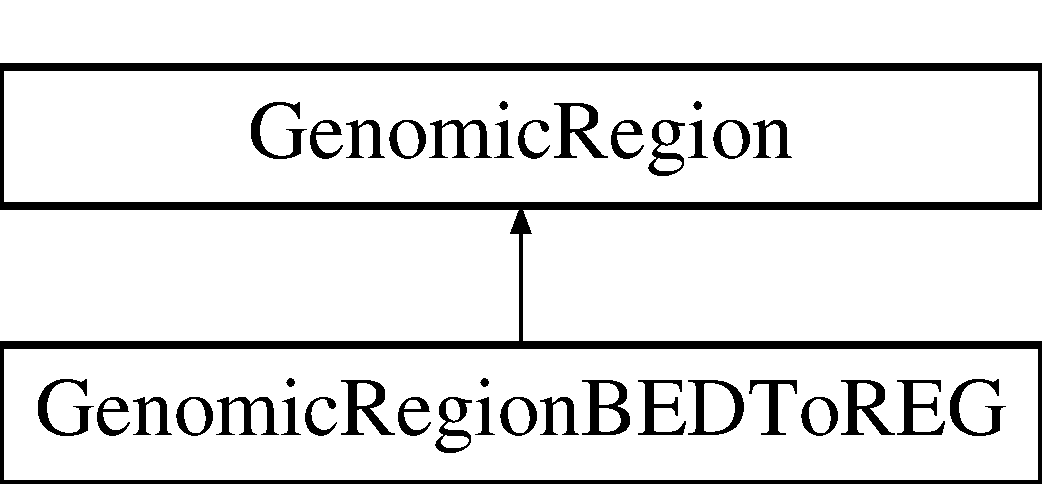
\includegraphics[height=2cm]{classGenomicRegionBEDToREG}
\end{center}
\end{figure}
\subsection*{Public Member Functions}
\begin{CompactItemize}
\item 
\hypertarget{classGenomicRegionBEDToREG_964b37e08c0c513d974e14cadaba5d20}{
\hyperlink{classGenomicRegionBEDToREG_964b37e08c0c513d974e14cadaba5d20}{GenomicRegionBEDToREG} (\hyperlink{classFileBuffer}{FileBuffer} $\ast$B)}
\label{classGenomicRegionBEDToREG_964b37e08c0c513d974e14cadaba5d20}

\begin{CompactList}\small\item\em Class constructor, see example below. \item\end{CompactList}\item 
\hypertarget{classGenomicRegionBEDToREG_b0fa681e5f8ddc81b0e27786bd86b9d9}{
\hyperlink{classGenomicRegionBEDToREG_b0fa681e5f8ddc81b0e27786bd86b9d9}{GenomicRegionBEDToREG} (char $\ast$inp, long int \hyperlink{classGenomicRegion_efe2255aeed5338060190ded05cb9c0c}{n\_\-line}=0)}
\label{classGenomicRegionBEDToREG_b0fa681e5f8ddc81b0e27786bd86b9d9}

\begin{CompactList}\small\item\em Class constructor, see example below. \item\end{CompactList}\item 
\hypertarget{classGenomicRegionBEDToREG_59650c4d898e5835271627bf8c45c609}{
\hyperlink{classGenomicRegionBEDToREG_59650c4d898e5835271627bf8c45c609}{$\sim$GenomicRegionBEDToREG} ()}
\label{classGenomicRegionBEDToREG_59650c4d898e5835271627bf8c45c609}

\begin{CompactList}\small\item\em Class destructor. \item\end{CompactList}\item 
\hypertarget{classGenomicRegionBEDToREG_3f18f7f3946f2258b30e9796fafee093}{
void \hyperlink{classGenomicRegionBEDToREG_3f18f7f3946f2258b30e9796fafee093}{Read} (char $\ast$inp, long int \hyperlink{classGenomicRegion_efe2255aeed5338060190ded05cb9c0c}{n\_\-line}=0)}
\label{classGenomicRegionBEDToREG_3f18f7f3946f2258b30e9796fafee093}

\begin{CompactList}\small\item\em Reads BED format from input string {\bf inp}. \item\end{CompactList}\end{CompactItemize}


\subsection{Detailed Description}
This class reads BED files but converts them internally to the REG format, so all operations are performed on the REG format. 

Example: 

\begin{Code}\begin{verbatim}    GenomicRegionBEDToREG x("chr1 132033 140102 Region#1 1000 + 132033 140102 0 2 3899,4104 0,3965");
    cout << "x = \n"; x.Print();
\end{verbatim}
\end{Code}

 

The documentation for this class was generated from the following files:\begin{CompactItemize}
\item 
genomic\_\-intervals.h\item 
genomic\_\-intervals.cpp\end{CompactItemize}

\hypertarget{classGenomicRegionGFF}{
\section{GenomicRegionGFF Class Reference}
\label{classGenomicRegionGFF}\index{GenomicRegionGFF@{GenomicRegionGFF}}
}


This class processes genomic regions in SAM format.  




{\ttfamily \#include $<$genomic\_\-intervals.h$>$}

Inheritance diagram for GenomicRegionGFF:\begin{figure}[H]
\begin{center}
\leavevmode
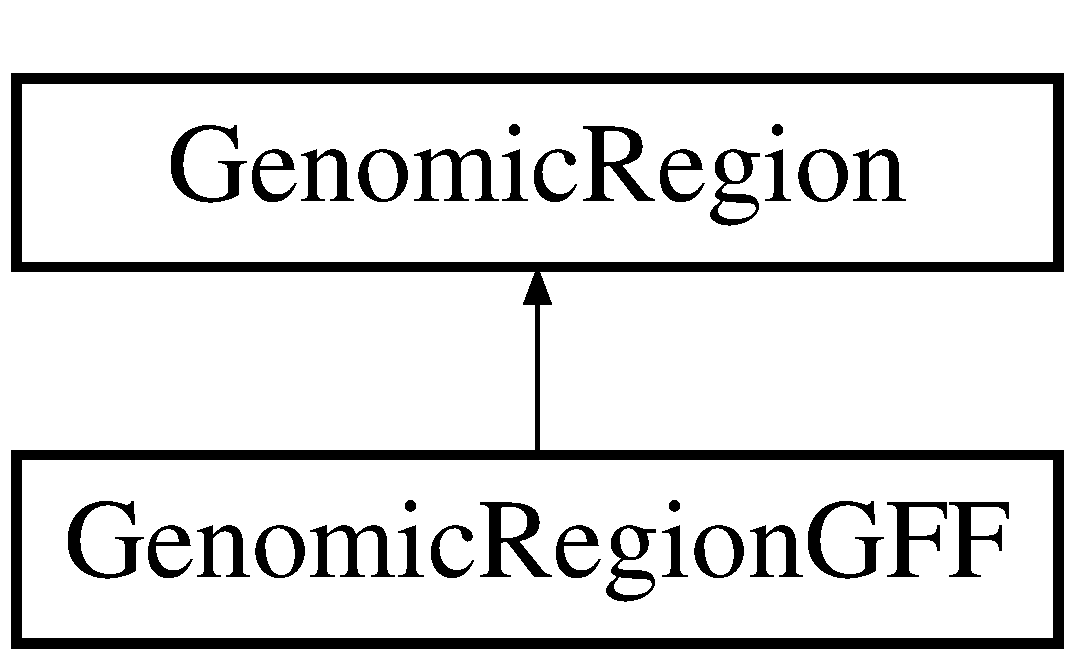
\includegraphics[height=2.000000cm]{classGenomicRegionGFF}
\end{center}
\end{figure}
\subsection*{Public Member Functions}
\begin{DoxyCompactItemize}
\item 
\hypertarget{classGenomicRegionGFF_a9a49f0dc39116964f774e7ce78cfc827}{
\hyperlink{classGenomicRegionGFF_a9a49f0dc39116964f774e7ce78cfc827}{GenomicRegionGFF} (\hyperlink{classFileBuffer}{FileBuffer} $\ast$B)}
\label{classGenomicRegionGFF_a9a49f0dc39116964f774e7ce78cfc827}

\begin{DoxyCompactList}\small\item\em Class constructor. \end{DoxyCompactList}\item 
\hypertarget{classGenomicRegionGFF_a59dee8d6f9e73b1da46386497030beb2}{
\hyperlink{classGenomicRegionGFF_a59dee8d6f9e73b1da46386497030beb2}{GenomicRegionGFF} (char $\ast$inp, long int \hyperlink{classGenomicRegion_aefe2255aeed5338060190ded05cb9c0c}{n\_\-line}=0)}
\label{classGenomicRegionGFF_a59dee8d6f9e73b1da46386497030beb2}

\begin{DoxyCompactList}\small\item\em Class constructor. \end{DoxyCompactList}\item 
\hypertarget{classGenomicRegionGFF_a3885d42a347283a5fed52791988076ad}{
\hyperlink{classGenomicRegionGFF_a3885d42a347283a5fed52791988076ad}{$\sim$GenomicRegionGFF} ()}
\label{classGenomicRegionGFF_a3885d42a347283a5fed52791988076ad}

\begin{DoxyCompactList}\small\item\em Class destructor. \end{DoxyCompactList}\item 
\hypertarget{classGenomicRegionGFF_aeb1390d42b388e32d98f58f57a5c169c}{
void \hyperlink{classGenomicRegionGFF_aeb1390d42b388e32d98f58f57a5c169c}{Read} (char $\ast$inp, long int \hyperlink{classGenomicRegion_aefe2255aeed5338060190ded05cb9c0c}{n\_\-line}=0)}
\label{classGenomicRegionGFF_aeb1390d42b388e32d98f58f57a5c169c}

\begin{DoxyCompactList}\small\item\em Reads GFF format from input string {\bfseries inp} \end{DoxyCompactList}\item 
\hypertarget{classGenomicRegionGFF_a3ffa71d729e4ff060a15a6bab1e924c8}{
void \hyperlink{classGenomicRegionGFF_a3ffa71d729e4ff060a15a6bab1e924c8}{Print} (FILE $\ast$file\_\-ptr=stdout)}
\label{classGenomicRegionGFF_a3ffa71d729e4ff060a15a6bab1e924c8}

\begin{DoxyCompactList}\small\item\em Prints label and genomic region intervals with a newline character at the end. \end{DoxyCompactList}\item 
\hypertarget{classGenomicRegionGFF_a96539f4372048c9f0d87826f5856a8ef}{
void \hyperlink{classGenomicRegionGFF_a96539f4372048c9f0d87826f5856a8ef}{PrintConstrained} (\hyperlink{classGenomicRegion}{GenomicRegion} $\ast$r, bool merge\_\-labels=false)}
\label{classGenomicRegionGFF_a96539f4372048c9f0d87826f5856a8ef}

\begin{DoxyCompactList}\small\item\em Same as \hyperlink{classGenomicRegionGFF_a3ffa71d729e4ff060a15a6bab1e924c8}{Print()}, but the interval is constrained between {\bfseries start} and {\bfseries stop} \end{DoxyCompactList}\item 
\hypertarget{classGenomicRegionGFF_a4b331cd12506aa4793a2cf6ea7620936}{
void \hyperlink{classGenomicRegionGFF_a4b331cd12506aa4793a2cf6ea7620936}{PrintModified} (char $\ast$label, long int start, long int stop)}
\label{classGenomicRegionGFF_a4b331cd12506aa4793a2cf6ea7620936}

\begin{DoxyCompactList}\small\item\em Same as \hyperlink{classGenomicRegionGFF_a3ffa71d729e4ff060a15a6bab1e924c8}{Print()}, but the label and interval's coordinates are modified. \end{DoxyCompactList}\item 
\hypertarget{classGenomicRegionGFF_aee70fcc81c9a6629bf0aa1ec37cb1d64}{
void \hyperlink{classGenomicRegionGFF_aee70fcc81c9a6629bf0aa1ec37cb1d64}{Diff} ()}
\label{classGenomicRegionGFF_aee70fcc81c9a6629bf0aa1ec37cb1d64}

\begin{DoxyCompactList}\small\item\em Replace regions with the corresponding gap intervals between successive intervals (e.g. used to compute intron boundaries) \end{DoxyCompactList}\item 
\hypertarget{classGenomicRegionGFF_a0ff4768578a03011fabad309072fade4}{
void \hyperlink{classGenomicRegionGFF_a0ff4768578a03011fabad309072fade4}{RunCalcDistances} (char $\ast$op1, char $\ast$op2)}
\label{classGenomicRegionGFF_a0ff4768578a03011fabad309072fade4}

\begin{DoxyCompactList}\small\item\em Print distance between successive intervals. \end{DoxyCompactList}\item 
\hypertarget{classGenomicRegionGFF_a77975c03dd39b404098eb519e81f67d4}{
void \hyperlink{classGenomicRegionGFF_a77975c03dd39b404098eb519e81f67d4}{Divide} ()}
\label{classGenomicRegionGFF_a77975c03dd39b404098eb519e81f67d4}

\begin{DoxyCompactList}\small\item\em Divide intervals divided in half (i.e. two intervals for each original interval in the genomic region) \end{DoxyCompactList}\item 
\hypertarget{classGenomicRegionGFF_ad4acc1231677efd876084ef36db82de1}{
void \hyperlink{classGenomicRegionGFF_ad4acc1231677efd876084ef36db82de1}{RunDivide} ()}
\label{classGenomicRegionGFF_ad4acc1231677efd876084ef36db82de1}

\begin{DoxyCompactList}\small\item\em Print intervals divided in half (i.e. two intervals for each original interval in the genomic region) \end{DoxyCompactList}\item 
\hypertarget{classGenomicRegionGFF_ad35d9b6e9c57270c0d5648ae9f702959}{
void \hyperlink{classGenomicRegionGFF_ad35d9b6e9c57270c0d5648ae9f702959}{Intersect} ()}
\label{classGenomicRegionGFF_ad35d9b6e9c57270c0d5648ae9f702959}

\begin{DoxyCompactList}\small\item\em Print intersection among all intervals, i.e. maximum start to minimum stop position. \end{DoxyCompactList}\item 
\hypertarget{classGenomicRegionGFF_aaa9b1271561e2d62ef1be6464e589cf4}{
void \hyperlink{classGenomicRegionGFF_aaa9b1271561e2d62ef1be6464e589cf4}{Select} (bool first, bool last, bool from5p, bool from3p)}
\label{classGenomicRegionGFF_aaa9b1271561e2d62ef1be6464e589cf4}

\begin{DoxyCompactList}\small\item\em Selects a subset of intervals according to their relative positions. \end{DoxyCompactList}\item 
\hypertarget{classGenomicRegionGFF_abc08552b0ad4ca512f79064b8cd64e54}{
void \hyperlink{classGenomicRegionGFF_abc08552b0ad4ca512f79064b8cd64e54}{RunSplit} ()}
\label{classGenomicRegionGFF_abc08552b0ad4ca512f79064b8cd64e54}

\begin{DoxyCompactList}\small\item\em Print region intervals on separate lines. \end{DoxyCompactList}\item 
\hypertarget{classGenomicRegionGFF_a3815f1b27aef231a674c527e11f25880}{
void \hyperlink{classGenomicRegionGFF_a3815f1b27aef231a674c527e11f25880}{PrintWindows} (long int win\_\-step, long int win\_\-size)}
\label{classGenomicRegionGFF_a3815f1b27aef231a674c527e11f25880}

\begin{DoxyCompactList}\small\item\em Print sliding windows (implemented only for single-\/interval regions) \end{DoxyCompactList}\end{DoxyCompactItemize}
\subsection*{Public Attributes}
\begin{DoxyCompactItemize}
\item 
\hypertarget{classGenomicRegionGFF_aaec963f555e7e807fb5046566622f5ee}{
long int \hyperlink{classGenomicRegionGFF_aaec963f555e7e807fb5046566622f5ee}{n\_\-tokens}}
\label{classGenomicRegionGFF_aaec963f555e7e807fb5046566622f5ee}

\begin{DoxyCompactList}\small\item\em number of TAB-\/separated fields in GFF entry (= 11) \end{DoxyCompactList}\item 
\hypertarget{classGenomicRegionGFF_a2f0d4a5f15d8a756233436af03341734}{
char $\ast$ \hyperlink{classGenomicRegionGFF_a2f0d4a5f15d8a756233436af03341734}{SOURCE}}
\label{classGenomicRegionGFF_a2f0d4a5f15d8a756233436af03341734}

\begin{DoxyCompactList}\small\item\em feature source \end{DoxyCompactList}\item 
\hypertarget{classGenomicRegionGFF_a0de447fbfad3da5b7a9cf07a5a6980f0}{
char $\ast$ \hyperlink{classGenomicRegionGFF_a0de447fbfad3da5b7a9cf07a5a6980f0}{FEATURE}}
\label{classGenomicRegionGFF_a0de447fbfad3da5b7a9cf07a5a6980f0}

\begin{DoxyCompactList}\small\item\em feture type \end{DoxyCompactList}\item 
\hypertarget{classGenomicRegionGFF_a0e92da1f0fd153504e0630f27229ba4d}{
char $\ast$ \hyperlink{classGenomicRegionGFF_a0e92da1f0fd153504e0630f27229ba4d}{SCORE}}
\label{classGenomicRegionGFF_a0e92da1f0fd153504e0630f27229ba4d}

\begin{DoxyCompactList}\small\item\em score \end{DoxyCompactList}\item 
\hypertarget{classGenomicRegionGFF_a42122a69eec385e0106e3861cb3b98f3}{
char \hyperlink{classGenomicRegionGFF_a42122a69eec385e0106e3861cb3b98f3}{FRAME}}
\label{classGenomicRegionGFF_a42122a69eec385e0106e3861cb3b98f3}

\begin{DoxyCompactList}\small\item\em coding frame \end{DoxyCompactList}\item 
\hypertarget{classGenomicRegionGFF_a625a023f1bb24fc597e723919a036073}{
char $\ast$ \hyperlink{classGenomicRegionGFF_a625a023f1bb24fc597e723919a036073}{COMMENT}}
\label{classGenomicRegionGFF_a625a023f1bb24fc597e723919a036073}

\begin{DoxyCompactList}\small\item\em comment \end{DoxyCompactList}\end{DoxyCompactItemize}


\subsection{Detailed Description}
This class processes genomic regions in SAM format. 

The documentation for this class was generated from the following files:\begin{DoxyCompactItemize}
\item 
genomic\_\-intervals.h\item 
genomic\_\-intervals.cpp\end{DoxyCompactItemize}

\hypertarget{classGenomicRegionGFFToREG}{
\section{GenomicRegionGFFToREG Class Reference}
\label{classGenomicRegionGFFToREG}\index{GenomicRegionGFFToREG@{GenomicRegionGFFToREG}}
}
This class reads GFF files but converts them internally to the REG format, so all operations are performed on the REG format.  


{\tt \#include $<$genomic\_\-intervals.h$>$}

Inheritance diagram for GenomicRegionGFFToREG::\begin{figure}[H]
\begin{center}
\leavevmode
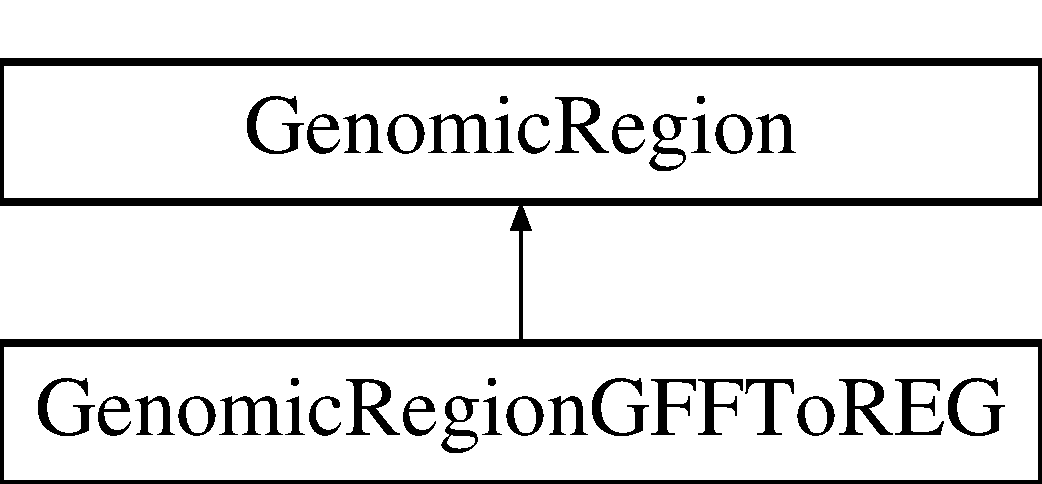
\includegraphics[height=2cm]{classGenomicRegionGFFToREG}
\end{center}
\end{figure}
\subsection*{Public Member Functions}
\begin{CompactItemize}
\item 
\hypertarget{classGenomicRegionGFFToREG_8ad38850fd8e7e19aabca0bf2ba62d55}{
\hyperlink{classGenomicRegionGFFToREG_8ad38850fd8e7e19aabca0bf2ba62d55}{GenomicRegionGFFToREG} (\hyperlink{classFileBuffer}{FileBuffer} $\ast$B)}
\label{classGenomicRegionGFFToREG_8ad38850fd8e7e19aabca0bf2ba62d55}

\begin{CompactList}\small\item\em Class constructor, see example below. \item\end{CompactList}\item 
\hypertarget{classGenomicRegionGFFToREG_fa25d23d19de119347fe6970913398b8}{
\hyperlink{classGenomicRegionGFFToREG_fa25d23d19de119347fe6970913398b8}{GenomicRegionGFFToREG} (char $\ast$inp, long int \hyperlink{classGenomicRegion_efe2255aeed5338060190ded05cb9c0c}{n\_\-line}=0)}
\label{classGenomicRegionGFFToREG_fa25d23d19de119347fe6970913398b8}

\begin{CompactList}\small\item\em Class constructor, see example below. \item\end{CompactList}\item 
\hypertarget{classGenomicRegionGFFToREG_5a41c3de64cd8ad69952b77805816c5e}{
\hyperlink{classGenomicRegionGFFToREG_5a41c3de64cd8ad69952b77805816c5e}{$\sim$GenomicRegionGFFToREG} ()}
\label{classGenomicRegionGFFToREG_5a41c3de64cd8ad69952b77805816c5e}

\begin{CompactList}\small\item\em Class destructor. \item\end{CompactList}\item 
\hypertarget{classGenomicRegionGFFToREG_bc519dd06e8d03711b90679ec279be3b}{
void \hyperlink{classGenomicRegionGFFToREG_bc519dd06e8d03711b90679ec279be3b}{Read} (char $\ast$inp, long int \hyperlink{classGenomicRegion_efe2255aeed5338060190ded05cb9c0c}{n\_\-line}=0)}
\label{classGenomicRegionGFFToREG_bc519dd06e8d03711b90679ec279be3b}

\begin{CompactList}\small\item\em Reads GFF format from input string {\bf inp}. \item\end{CompactList}\end{CompactItemize}


\subsection{Detailed Description}
This class reads GFF files but converts them internally to the REG format, so all operations are performed on the REG format. 

The documentation for this class was generated from the following files:\begin{CompactItemize}
\item 
genomic\_\-intervals.h\item 
genomic\_\-intervals.cpp\end{CompactItemize}

\hypertarget{classGenomicRegionSAM}{
\section{GenomicRegionSAM Class Reference}
\label{classGenomicRegionSAM}\index{GenomicRegionSAM@{GenomicRegionSAM}}
}
This class processes genomic regions in SAM format.  


{\tt \#include $<$genomic\_\-intervals.h$>$}

Inheritance diagram for GenomicRegionSAM::\begin{figure}[H]
\begin{center}
\leavevmode
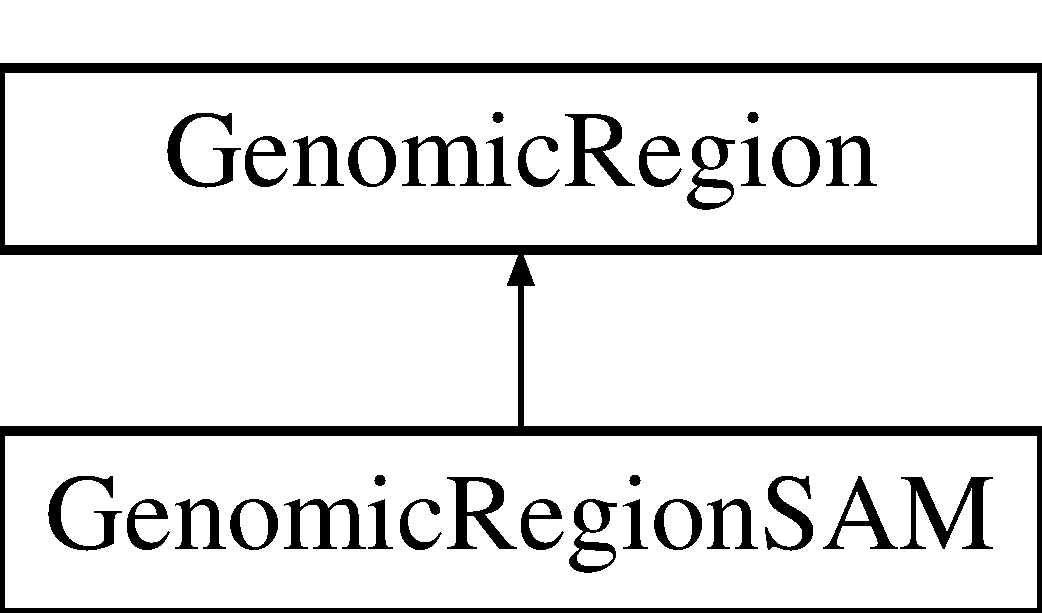
\includegraphics[height=2cm]{classGenomicRegionSAM}
\end{center}
\end{figure}
\subsection*{Public Types}
\begin{CompactItemize}
\item 
\hypertarget{classGenomicRegionSAM_adf8580c5362304ab4866fa76a59df96}{
typedef vector$<$ pair$<$ long int, char $>$ $>$ \hyperlink{classGenomicRegionSAM_adf8580c5362304ab4866fa76a59df96}{CIGARTokens}}
\label{classGenomicRegionSAM_adf8580c5362304ab4866fa76a59df96}

\begin{CompactList}\small\item\em This type is used for storing CIGAR tokens, i.e. (token\_\-type, token\_\-length). \item\end{CompactList}\end{CompactItemize}
\subsection*{Public Member Functions}
\begin{CompactItemize}
\item 
\hypertarget{classGenomicRegionSAM_e6b0828926a573743e7292567346c1a1}{
\hyperlink{classGenomicRegionSAM_e6b0828926a573743e7292567346c1a1}{GenomicRegionSAM} (\hyperlink{classFileBuffer}{FileBuffer} $\ast$B)}
\label{classGenomicRegionSAM_e6b0828926a573743e7292567346c1a1}

\begin{CompactList}\small\item\em Class constructor. \item\end{CompactList}\item 
\hypertarget{classGenomicRegionSAM_25247d97947a54583fb17d493df4a0cf}{
\hyperlink{classGenomicRegionSAM_25247d97947a54583fb17d493df4a0cf}{GenomicRegionSAM} (char $\ast$inp, long int \hyperlink{classGenomicRegion_efe2255aeed5338060190ded05cb9c0c}{n\_\-line}=0)}
\label{classGenomicRegionSAM_25247d97947a54583fb17d493df4a0cf}

\begin{CompactList}\small\item\em Class constructor. \item\end{CompactList}\item 
\hypertarget{classGenomicRegionSAM_1d11cc22134d13dbf67ffe4c7220888d}{
\hyperlink{classGenomicRegionSAM_1d11cc22134d13dbf67ffe4c7220888d}{$\sim$GenomicRegionSAM} ()}
\label{classGenomicRegionSAM_1d11cc22134d13dbf67ffe4c7220888d}

\begin{CompactList}\small\item\em Class destructor. \item\end{CompactList}\item 
\hypertarget{classGenomicRegionSAM_096d90b6743400daf1acb50bcf17086a}{
void \hyperlink{classGenomicRegionSAM_096d90b6743400daf1acb50bcf17086a}{Read} (char $\ast$inp, long int \hyperlink{classGenomicRegion_efe2255aeed5338060190ded05cb9c0c}{n\_\-line}=0)}
\label{classGenomicRegionSAM_096d90b6743400daf1acb50bcf17086a}

\begin{CompactList}\small\item\em Reads SAM format from input string {\bf inp}. \item\end{CompactList}\item 
\hypertarget{classGenomicRegionSAM_4381c6486f767b6e4055cb729beee181}{
void \hyperlink{classGenomicRegionSAM_4381c6486f767b6e4055cb729beee181}{Print} (FILE $\ast$file\_\-ptr=stdout)}
\label{classGenomicRegionSAM_4381c6486f767b6e4055cb729beee181}

\begin{CompactList}\small\item\em Prints label and genomic region intervals with a newline character at the end. \item\end{CompactList}\item 
\hypertarget{classGenomicRegionSAM_df8beab78f541121e7b56957afffa4ac}{
void \hyperlink{classGenomicRegionSAM_df8beab78f541121e7b56957afffa4ac}{PrintConstrained} (\hyperlink{classGenomicRegion}{GenomicRegion} $\ast$r, bool merge\_\-labels=false)}
\label{classGenomicRegionSAM_df8beab78f541121e7b56957afffa4ac}

\begin{CompactList}\small\item\em Same as \hyperlink{classGenomicRegionSAM_4381c6486f767b6e4055cb729beee181}{Print()}, but the interval is constrained between {\bf start} and {\bf stop}. \item\end{CompactList}\item 
\hypertarget{classGenomicRegionSAM_ecf1d74c572e85bbe9bca0b30c6a6dda}{
void \hyperlink{classGenomicRegionSAM_ecf1d74c572e85bbe9bca0b30c6a6dda}{PrintModified} (char $\ast$label, long int start, long int stop)}
\label{classGenomicRegionSAM_ecf1d74c572e85bbe9bca0b30c6a6dda}

\begin{CompactList}\small\item\em Same as \hyperlink{classGenomicRegionSAM_4381c6486f767b6e4055cb729beee181}{Print()}, but the label and interval's coordinates are modified. \item\end{CompactList}\item 
\hypertarget{classGenomicRegionSAM_6d0949a836520073de57e0f968a6b819}{
char \hyperlink{classGenomicRegionSAM_6d0949a836520073de57e0f968a6b819}{CalcStrandFromFlag} (unsigned long int flag)}
\label{classGenomicRegionSAM_6d0949a836520073de57e0f968a6b819}

\begin{CompactList}\small\item\em Extracts the strand from the FLAG field. \item\end{CompactList}\item 
\hypertarget{classGenomicRegionSAM_f583a963f7fb0eb071c1b640c660813a}{
void \hyperlink{classGenomicRegionSAM_f583a963f7fb0eb071c1b640c660813a}{UpdateFlagFromStrand} (char strand)}
\label{classGenomicRegionSAM_f583a963f7fb0eb071c1b640c660813a}

\begin{CompactList}\small\item\em Updates the FLAG field given a new strand. \item\end{CompactList}\item 
\hypertarget{classGenomicRegionSAM_ea563a4a484784ad231399a3b56c7056}{
void \hyperlink{classGenomicRegionSAM_ea563a4a484784ad231399a3b56c7056}{PrintGappedSequence} (char $\ast$seq, char $\ast$gap\_\-token\_\-types, bool lowercase\_\-for\_\-sort\_\-clipping=true)}
\label{classGenomicRegionSAM_ea563a4a484784ad231399a3b56c7056}

\begin{CompactList}\small\item\em Prints gapped sequence. \item\end{CompactList}\item 
\hypertarget{classGenomicRegionSAM_9446540150b384ca0d3dbba630c9c6a6}{
char $\ast$ \hyperlink{classGenomicRegionSAM_9446540150b384ca0d3dbba630c9c6a6}{GetGappedSequence} (char $\ast$seq, char $\ast$gap\_\-token\_\-types, bool lowercase\_\-for\_\-sort\_\-clipping=true)}
\label{classGenomicRegionSAM_9446540150b384ca0d3dbba630c9c6a6}

\begin{CompactList}\small\item\em Returns gapped sequence. \item\end{CompactList}\item 
\hypertarget{classGenomicRegionSAM_621b3dd6f4d03a5223bd26a57af14f7e}{
void \hyperlink{classGenomicRegionSAM_621b3dd6f4d03a5223bd26a57af14f7e}{InvalidateSeqData} ()}
\label{classGenomicRegionSAM_621b3dd6f4d03a5223bd26a57af14f7e}

\begin{CompactList}\small\item\em Sets CIGAR, SEQ and QUAL fields to \char`\"{}$\ast$\char`\"{} and removes OPTIONAL field; also \hyperlink{classGenomicRegionSAM_281e35ef1bd0b7da811d9b8957f3d08f}{GenomicRegionSAM::n\_\-tokens} is set to 11. \item\end{CompactList}\item 
\hypertarget{classGenomicRegionSAM_34b0387b9656e48d0c4046d62fe085e1}{
void \hyperlink{classGenomicRegionSAM_34b0387b9656e48d0c4046d62fe085e1}{TokenizeCIGAR} ()}
\label{classGenomicRegionSAM_34b0387b9656e48d0c4046d62fe085e1}

\begin{CompactList}\small\item\em Computes and stores CIGAR tokens in \hyperlink{classGenomicRegionSAM_47afdde68b89cf4ea199bc91d4954a92}{GenomicRegionSAM::T}. \item\end{CompactList}\item 
\hypertarget{classGenomicRegionSAM_50198fead1c40caadf76f40b61a3c14a}{
long int \hyperlink{classGenomicRegionSAM_50198fead1c40caadf76f40b61a3c14a}{GetNextTokenOfCIGAR} (char $\ast$$\ast$cigar, char $\ast$type)}
\label{classGenomicRegionSAM_50198fead1c40caadf76f40b61a3c14a}

\begin{CompactList}\small\item\em Returns next token in CIGAR string. \item\end{CompactList}\item 
\hypertarget{classGenomicRegionSAM_965bb3cc1217e6c859a07dd23090c2a0}{
void \hyperlink{classGenomicRegionSAM_965bb3cc1217e6c859a07dd23090c2a0}{UpdateCigarFromIntervals} ()}
\label{classGenomicRegionSAM_965bb3cc1217e6c859a07dd23090c2a0}

\begin{CompactList}\small\item\em Update CIGAR string based only on interval information (chooses simplest possible CIGAR). \item\end{CompactList}\item 
\hypertarget{classGenomicRegionSAM_5de5d05dfccd33149153a299c1cb2f6b}{
long int \hyperlink{classGenomicRegionSAM_5de5d05dfccd33149153a299c1cb2f6b}{CalcFragmentLengthFromCIGAR} ()}
\label{classGenomicRegionSAM_5de5d05dfccd33149153a299c1cb2f6b}

\begin{CompactList}\small\item\em Calculate interval length from CIGAR string. \item\end{CompactList}\item 
\hypertarget{classGenomicRegionSAM_acff4cd74a3b8c450f9f90c6b23412c4}{
long int \hyperlink{classGenomicRegionSAM_acff4cd74a3b8c450f9f90c6b23412c4}{CalcReferenceLengthFromCIGAR} ()}
\label{classGenomicRegionSAM_acff4cd74a3b8c450f9f90c6b23412c4}

\begin{CompactList}\small\item\em Calculate interval length from CIGAR string. \item\end{CompactList}\item 
\hypertarget{classGenomicRegionSAM_17e8e7054ffe7205d7c34926b60526d8}{
char $\ast$ \hyperlink{classGenomicRegionSAM_17e8e7054ffe7205d7c34926b60526d8}{TrimCIGAR} (long int d\_\-ref\_\-start, long int d\_\-ref\_\-stop)}
\label{classGenomicRegionSAM_17e8e7054ffe7205d7c34926b60526d8}

\begin{CompactList}\small\item\em Trim CIGAR string from left and right by a given distance (measured on the reference sequence). \item\end{CompactList}\item 
\hypertarget{classGenomicRegionSAM_0ff4472118291a8034efc929c784680c}{
char $\ast$ \hyperlink{classGenomicRegionSAM_0ff4472118291a8034efc929c784680c}{TrimSequence} (char $\ast$seq, long int d\_\-ref\_\-start, long int d\_\-ref\_\-stop)}
\label{classGenomicRegionSAM_0ff4472118291a8034efc929c784680c}

\begin{CompactList}\small\item\em Trim input {\bf seq} from left and right (used for trimming both SEQ and QUAL fields). \item\end{CompactList}\item 
\hypertarget{classGenomicRegionSAM_97b9fec94e5f21490d839b3f99235a96}{
void \hyperlink{classGenomicRegionSAM_97b9fec94e5f21490d839b3f99235a96}{RunAlign} (\hyperlink{classChromosomes}{Chromosomes} $\ast$C)}
\label{classGenomicRegionSAM_97b9fec94e5f21490d839b3f99235a96}

\begin{CompactList}\small\item\em Prints alignments of input sequences to reference genome. \item\end{CompactList}\item 
\hypertarget{classGenomicRegionSAM_5d82c1d84432274392416f87bfac655a}{
void \hyperlink{classGenomicRegionSAM_5d82c1d84432274392416f87bfac655a}{ApplyBounds} (StringLIntMap $\ast$bounds)}
\label{classGenomicRegionSAM_5d82c1d84432274392416f87bfac655a}

\begin{CompactList}\small\item\em Corrects interval start/stop positions so as to comply with chromosomal bounds. \item\end{CompactList}\item 
\hypertarget{classGenomicRegionSAM_52fa8c0420b16fe92f54427365f72899}{
void \hyperlink{classGenomicRegionSAM_52fa8c0420b16fe92f54427365f72899}{Center} ()}
\label{classGenomicRegionSAM_52fa8c0420b16fe92f54427365f72899}

\begin{CompactList}\small\item\em Replace each interval in the region with the corresponding center interval. \item\end{CompactList}\item 
\hypertarget{classGenomicRegionSAM_d765c84814151be0e710fefb37c7949a}{
void \hyperlink{classGenomicRegionSAM_d765c84814151be0e710fefb37c7949a}{Connect} ()}
\label{classGenomicRegionSAM_d765c84814151be0e710fefb37c7949a}

\begin{CompactList}\small\item\em Replace region with a single interval from minimum start to maximum stop position. \item\end{CompactList}\item 
\hypertarget{classGenomicRegionSAM_ca38b04fa916ae4c9c28c36f537136ba}{
void \hyperlink{classGenomicRegionSAM_ca38b04fa916ae4c9c28c36f537136ba}{Diff} ()}
\label{classGenomicRegionSAM_ca38b04fa916ae4c9c28c36f537136ba}

\begin{CompactList}\small\item\em Replace regions with the corresponding gap intervals between successive intervals (e.g. used to compute intron boundaries). \item\end{CompactList}\item 
\hypertarget{classGenomicRegionSAM_fc9c7ec17be517dd5b1ad7cb62f58826}{
void \hyperlink{classGenomicRegionSAM_fc9c7ec17be517dd5b1ad7cb62f58826}{RunCalcDistances} (char $\ast$op1, char $\ast$op2)}
\label{classGenomicRegionSAM_fc9c7ec17be517dd5b1ad7cb62f58826}

\begin{CompactList}\small\item\em Print distance between successive intervals. \item\end{CompactList}\item 
\hypertarget{classGenomicRegionSAM_7c16ba87be562950021d3f19eb14ac5e}{
void \hyperlink{classGenomicRegionSAM_7c16ba87be562950021d3f19eb14ac5e}{Divide} ()}
\label{classGenomicRegionSAM_7c16ba87be562950021d3f19eb14ac5e}

\begin{CompactList}\small\item\em Divide intervals divided in half (i.e. two intervals for each original interval in the genomic region). \item\end{CompactList}\item 
\hypertarget{classGenomicRegionSAM_dd2ada73e241f593dcdcdfca97df1eb5}{
void \hyperlink{classGenomicRegionSAM_dd2ada73e241f593dcdcdfca97df1eb5}{RunDivide} ()}
\label{classGenomicRegionSAM_dd2ada73e241f593dcdcdfca97df1eb5}

\begin{CompactList}\small\item\em Print intervals divided in half (i.e. two intervals for each original interval in the genomic region). \item\end{CompactList}\item 
\hypertarget{classGenomicRegionSAM_d955a6a512678613b4a42d2db0d3f549}{
void \hyperlink{classGenomicRegionSAM_d955a6a512678613b4a42d2db0d3f549}{Fix} ()}
\label{classGenomicRegionSAM_d955a6a512678613b4a42d2db0d3f549}

\begin{CompactList}\small\item\em Removes rogue intervals (e.g. start$>$stop). \item\end{CompactList}\item 
\hypertarget{classGenomicRegionSAM_4f26b01325ebd4e20c9bf3247d5fa733}{
void \hyperlink{classGenomicRegionSAM_4f26b01325ebd4e20c9bf3247d5fa733}{Intersect} ()}
\label{classGenomicRegionSAM_4f26b01325ebd4e20c9bf3247d5fa733}

\begin{CompactList}\small\item\em Print intersection among all intervals, i.e. maximum start to minimum stop position. \item\end{CompactList}\item 
\hypertarget{classGenomicRegionSAM_538b8fc9969f24da6911ec39c8d70a3b}{
void \hyperlink{classGenomicRegionSAM_538b8fc9969f24da6911ec39c8d70a3b}{Randomize} (gsl\_\-rng $\ast$random\_\-generator, StringLIntMap $\ast$bounds)}
\label{classGenomicRegionSAM_538b8fc9969f24da6911ec39c8d70a3b}

\begin{CompactList}\small\item\em Randomizes interval position within chromosomal bounds. \item\end{CompactList}\item 
void \hyperlink{classGenomicRegionSAM_353207352073db00dee0a9b620dca197}{ModifyPos} (char $\ast$position\_\-op, long int position\_\-shift)
\begin{CompactList}\small\item\em Modifies interval start/stop positions. First it chooses which position to keep fixed, and then it shifts the non-fixed position. \item\end{CompactList}\item 
\hypertarget{classGenomicRegionSAM_4dce925fdb55dcc7ef3dad890bc25408}{
void \hyperlink{classGenomicRegionSAM_4dce925fdb55dcc7ef3dad890bc25408}{Select} (bool first, bool last, bool from5p, bool from3p)}
\label{classGenomicRegionSAM_4dce925fdb55dcc7ef3dad890bc25408}

\begin{CompactList}\small\item\em Selects a subset of intervals according to their relative positions. \item\end{CompactList}\item 
void \hyperlink{classGenomicRegionSAM_fb2701ba1a521ae2c07ea0ace2f9ee77}{ShiftPos} (long int start\_\-shift, long int stop\_\-shift, bool strand\_\-aware)
\begin{CompactList}\small\item\em Shifts interval start/stop positions. First it chooses reference position, and then shifts start and stop positions separately. \item\end{CompactList}\item 
\hypertarget{classGenomicRegionSAM_b31fed1760d543fa3a38bb16a064dcf9}{
void \hyperlink{classGenomicRegionSAM_b31fed1760d543fa3a38bb16a064dcf9}{RunShuffle} (gsl\_\-rng $\ast$random\_\-generator, \hyperlink{classGenomicRegionSet}{GenomicRegionSet} $\ast$refReg, StringLIntMap $\ast$index, StringVecLIntMap $\ast$loc)}
\label{classGenomicRegionSAM_b31fed1760d543fa3a38bb16a064dcf9}

\begin{CompactList}\small\item\em Prints shuffled region within specified reference regions in {\bf refReg}. \item\end{CompactList}\item 
\hypertarget{classGenomicRegionSAM_8a27afdcdf11895d7b3f32bd8eed68ae}{
void \hyperlink{classGenomicRegionSAM_8a27afdcdf11895d7b3f32bd8eed68ae}{Sort} ()}
\label{classGenomicRegionSAM_8a27afdcdf11895d7b3f32bd8eed68ae}

\begin{CompactList}\small\item\em Sort intervals according to start position (only for compatible intervals). \item\end{CompactList}\item 
\hypertarget{classGenomicRegionSAM_e195a95ba837bfd9673093f1d451b39c}{
void \hyperlink{classGenomicRegionSAM_e195a95ba837bfd9673093f1d451b39c}{RunSplit} ()}
\label{classGenomicRegionSAM_e195a95ba837bfd9673093f1d451b39c}

\begin{CompactList}\small\item\em Print region intervals on separate lines. \item\end{CompactList}\item 
\hypertarget{classGenomicRegionSAM_beb76df49bb89ecf0f3074805d9fe7b2}{
void \hyperlink{classGenomicRegionSAM_beb76df49bb89ecf0f3074805d9fe7b2}{ModifyStrand} (char $\ast$strand\_\-op)}
\label{classGenomicRegionSAM_beb76df49bb89ecf0f3074805d9fe7b2}

\begin{CompactList}\small\item\em Modified strand information: '+'=only forward, '-'=only reverse, 'r'=reverse strands from '+' to '-' and vice versa, 'b'=both strands. \item\end{CompactList}\item 
\hypertarget{classGenomicRegionSAM_6161ba10d2a4871cc43aa5bc597a787b}{
void \hyperlink{classGenomicRegionSAM_6161ba10d2a4871cc43aa5bc597a787b}{Union} ()}
\label{classGenomicRegionSAM_6161ba10d2a4871cc43aa5bc597a787b}

\begin{CompactList}\small\item\em Compute intervals' union. \item\end{CompactList}\item 
\hypertarget{classGenomicRegionSAM_27027bc80a3b5a864ebafd415a6ef5a6}{
void \hyperlink{classGenomicRegionSAM_27027bc80a3b5a864ebafd415a6ef5a6}{PrintWindows} (long int win\_\-step, long int win\_\-size)}
\label{classGenomicRegionSAM_27027bc80a3b5a864ebafd415a6ef5a6}

\begin{CompactList}\small\item\em Print sliding windows (implemented only for single-interval regions). \item\end{CompactList}\end{CompactItemize}
\subsection*{Public Attributes}
\begin{CompactItemize}
\item 
\hypertarget{classGenomicRegionSAM_281e35ef1bd0b7da811d9b8957f3d08f}{
long int \hyperlink{classGenomicRegionSAM_281e35ef1bd0b7da811d9b8957f3d08f}{n\_\-tokens}}
\label{classGenomicRegionSAM_281e35ef1bd0b7da811d9b8957f3d08f}

\begin{CompactList}\small\item\em number of TAB-separated fields in SAM entry ($>$= 12) \item\end{CompactList}\item 
\hypertarget{classGenomicRegionSAM_200d7f7044dd69311eceb851a3c315e5}{
unsigned long int \hyperlink{classGenomicRegionSAM_200d7f7044dd69311eceb851a3c315e5}{FLAG}}
\label{classGenomicRegionSAM_200d7f7044dd69311eceb851a3c315e5}

\begin{CompactList}\small\item\em bitwise FLAG \item\end{CompactList}\item 
\hypertarget{classGenomicRegionSAM_edacdd8319f4b614229a41b80d4c6f67}{
long int \hyperlink{classGenomicRegionSAM_edacdd8319f4b614229a41b80d4c6f67}{MAPQ}}
\label{classGenomicRegionSAM_edacdd8319f4b614229a41b80d4c6f67}

\begin{CompactList}\small\item\em MAPping Quality. \item\end{CompactList}\item 
\hypertarget{classGenomicRegionSAM_a5acff481ae565db4976e66933212726}{
char $\ast$ \hyperlink{classGenomicRegionSAM_a5acff481ae565db4976e66933212726}{CIGAR}}
\label{classGenomicRegionSAM_a5acff481ae565db4976e66933212726}

\begin{CompactList}\small\item\em CIGAR string. \item\end{CompactList}\item 
\hypertarget{classGenomicRegionSAM_f723505bfafff1a1fa616479023d0c3c}{
char $\ast$ \hyperlink{classGenomicRegionSAM_f723505bfafff1a1fa616479023d0c3c}{RNEXT}}
\label{classGenomicRegionSAM_f723505bfafff1a1fa616479023d0c3c}

\begin{CompactList}\small\item\em Reference name of the mate/next fragment. \item\end{CompactList}\item 
\hypertarget{classGenomicRegionSAM_d6f88b4324ba508b86102641d819661f}{
long int \hyperlink{classGenomicRegionSAM_d6f88b4324ba508b86102641d819661f}{PNEXT}}
\label{classGenomicRegionSAM_d6f88b4324ba508b86102641d819661f}

\begin{CompactList}\small\item\em Position of the mate/next fragment. \item\end{CompactList}\item 
\hypertarget{classGenomicRegionSAM_f180854a186be37eab49520edaa1262f}{
long int \hyperlink{classGenomicRegionSAM_f180854a186be37eab49520edaa1262f}{TLEN}}
\label{classGenomicRegionSAM_f180854a186be37eab49520edaa1262f}

\begin{CompactList}\small\item\em observed Template LENgth \item\end{CompactList}\item 
\hypertarget{classGenomicRegionSAM_6c2887ed1fa3a25d801641ea1b139032}{
char $\ast$ \hyperlink{classGenomicRegionSAM_6c2887ed1fa3a25d801641ea1b139032}{SEQ}}
\label{classGenomicRegionSAM_6c2887ed1fa3a25d801641ea1b139032}

\begin{CompactList}\small\item\em fragment SEQuence \item\end{CompactList}\item 
\hypertarget{classGenomicRegionSAM_b43ca5f2fbfdee520f1424c3a9fd0706}{
char $\ast$ \hyperlink{classGenomicRegionSAM_b43ca5f2fbfdee520f1424c3a9fd0706}{QUAL}}
\label{classGenomicRegionSAM_b43ca5f2fbfdee520f1424c3a9fd0706}

\begin{CompactList}\small\item\em ASCII of Phred-scaled base QUALity+33. \item\end{CompactList}\item 
\hypertarget{classGenomicRegionSAM_1622a8804462bad83b1c49d25eeacb49}{
char $\ast$ \hyperlink{classGenomicRegionSAM_1622a8804462bad83b1c49d25eeacb49}{OPTIONAL}}
\label{classGenomicRegionSAM_1622a8804462bad83b1c49d25eeacb49}

\begin{CompactList}\small\item\em all SAM fields after the 12th mandatory field \item\end{CompactList}\item 
\hypertarget{classGenomicRegionSAM_47afdde68b89cf4ea199bc91d4954a92}{
\hyperlink{classGenomicRegionSAM_adf8580c5362304ab4866fa76a59df96}{CIGARTokens} \hyperlink{classGenomicRegionSAM_47afdde68b89cf4ea199bc91d4954a92}{T}}
\label{classGenomicRegionSAM_47afdde68b89cf4ea199bc91d4954a92}

\begin{CompactList}\small\item\em CIGAR tokens. \item\end{CompactList}\end{CompactItemize}


\subsection{Detailed Description}
This class processes genomic regions in SAM format. 

\subsection{Member Function Documentation}
\hypertarget{classGenomicRegionSAM_353207352073db00dee0a9b620dca197}{
\index{GenomicRegionSAM@{GenomicRegionSAM}!ModifyPos@{ModifyPos}}
\index{ModifyPos@{ModifyPos}!GenomicRegionSAM@{GenomicRegionSAM}}
\subsubsection[ModifyPos]{\setlength{\rightskip}{0pt plus 5cm}void GenomicRegionSAM::ModifyPos (char $\ast$ {\em position\_\-op}, \/  long int {\em position\_\-shift})\hspace{0.3cm}{\tt  \mbox{[}virtual\mbox{]}}}}
\label{classGenomicRegionSAM_353207352073db00dee0a9b620dca197}


Modifies interval start/stop positions. First it chooses which position to keep fixed, and then it shifts the non-fixed position. 

\begin{Desc}
\item[Parameters:]
\begin{description}
\item[{\em position\_\-op}]selects fixed position as follows: '1'=start position, 'c'=center position, '5p'=5-prime, '3p'=3-prime \item[{\em position\_\-shift}]determines the shift of the non-fixed position (in the 'c' case, both positions are shifted symmetrically around the center) \end{description}
\end{Desc}


Reimplemented from \hyperlink{classGenomicRegion_0721b07af0850057e4ab9cd416ecac2f}{GenomicRegion}.\hypertarget{classGenomicRegionSAM_fb2701ba1a521ae2c07ea0ace2f9ee77}{
\index{GenomicRegionSAM@{GenomicRegionSAM}!ShiftPos@{ShiftPos}}
\index{ShiftPos@{ShiftPos}!GenomicRegionSAM@{GenomicRegionSAM}}
\subsubsection[ShiftPos]{\setlength{\rightskip}{0pt plus 5cm}void GenomicRegionSAM::ShiftPos (long int {\em start\_\-shift}, \/  long int {\em stop\_\-shift}, \/  bool {\em strand\_\-aware})\hspace{0.3cm}{\tt  \mbox{[}virtual\mbox{]}}}}
\label{classGenomicRegionSAM_fb2701ba1a521ae2c07ea0ace2f9ee77}


Shifts interval start/stop positions. First it chooses reference position, and then shifts start and stop positions separately. 

\begin{Desc}
\item[Parameters:]
\begin{description}
\item[{\em start\_\-shift}]determines the shift of the start position \item[{\em stop\_\-shift}]determines the shift of the stop position \item[{\em strand\_\-aware}]if 'true', then start=5-prime and stop=3-prime \end{description}
\end{Desc}


Reimplemented from \hyperlink{classGenomicRegion_0ee8c165839c79afdc586f8b5e07788e}{GenomicRegion}.

The documentation for this class was generated from the following files:\begin{CompactItemize}
\item 
genomic\_\-intervals.h\item 
genomic\_\-intervals.cpp\end{CompactItemize}

\hypertarget{classGenomicRegionSAMToREG}{
\section{GenomicRegionSAMToREG Class Reference}
\label{classGenomicRegionSAMToREG}\index{GenomicRegionSAMToREG@{GenomicRegionSAMToREG}}
}


This class reads SAM files but converts them internally to the REG format, so all operations are performed on the REG format.  




{\ttfamily \#include $<$genomic\_\-intervals.h$>$}

Inheritance diagram for GenomicRegionSAMToREG:\begin{figure}[H]
\begin{center}
\leavevmode
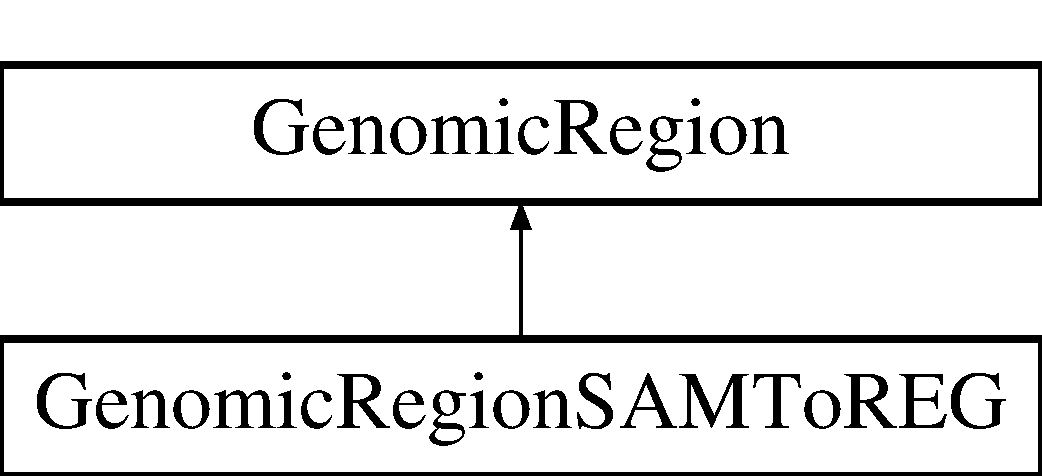
\includegraphics[height=2.000000cm]{classGenomicRegionSAMToREG}
\end{center}
\end{figure}
\subsection*{Public Member Functions}
\begin{DoxyCompactItemize}
\item 
\hypertarget{classGenomicRegionSAMToREG_a67555a42a7bba86d7e0389a09d1e3407}{
\hyperlink{classGenomicRegionSAMToREG_a67555a42a7bba86d7e0389a09d1e3407}{GenomicRegionSAMToREG} (\hyperlink{classFileBuffer}{FileBuffer} $\ast$B)}
\label{classGenomicRegionSAMToREG_a67555a42a7bba86d7e0389a09d1e3407}

\begin{DoxyCompactList}\small\item\em Class constructor, see example below. \end{DoxyCompactList}\item 
\hypertarget{classGenomicRegionSAMToREG_ad29083be26f4117ba4af3f265716b9ad}{
\hyperlink{classGenomicRegionSAMToREG_ad29083be26f4117ba4af3f265716b9ad}{GenomicRegionSAMToREG} (char $\ast$inp, long int \hyperlink{classGenomicRegion_aefe2255aeed5338060190ded05cb9c0c}{n\_\-line}=0)}
\label{classGenomicRegionSAMToREG_ad29083be26f4117ba4af3f265716b9ad}

\begin{DoxyCompactList}\small\item\em Class constructor, see example below. \end{DoxyCompactList}\item 
\hypertarget{classGenomicRegionSAMToREG_a19dea1653efdc013f4425a43470eab02}{
\hyperlink{classGenomicRegionSAMToREG_a19dea1653efdc013f4425a43470eab02}{$\sim$GenomicRegionSAMToREG} ()}
\label{classGenomicRegionSAMToREG_a19dea1653efdc013f4425a43470eab02}

\begin{DoxyCompactList}\small\item\em Class destructor. \end{DoxyCompactList}\item 
\hypertarget{classGenomicRegionSAMToREG_ab4a3b874cafac1537a7d7287cae39e76}{
void \hyperlink{classGenomicRegionSAMToREG_ab4a3b874cafac1537a7d7287cae39e76}{Read} (char $\ast$inp, long int \hyperlink{classGenomicRegion_aefe2255aeed5338060190ded05cb9c0c}{n\_\-line}=0)}
\label{classGenomicRegionSAMToREG_ab4a3b874cafac1537a7d7287cae39e76}

\begin{DoxyCompactList}\small\item\em Reads SAM format from input string {\bfseries inp} \end{DoxyCompactList}\item 
\hypertarget{classGenomicRegionSAMToREG_acc2044e03dc7e75bdcada1eb1e77a5ea}{
char \hyperlink{classGenomicRegionSAMToREG_acc2044e03dc7e75bdcada1eb1e77a5ea}{CalcStrandFromFlag} (unsigned long int flag)}
\label{classGenomicRegionSAMToREG_acc2044e03dc7e75bdcada1eb1e77a5ea}

\begin{DoxyCompactList}\small\item\em Extracts the strand from the FLAG field. \end{DoxyCompactList}\item 
\hypertarget{classGenomicRegionSAMToREG_adbc035818bcc64cc715b16c34b314799}{
long int \hyperlink{classGenomicRegionSAMToREG_adbc035818bcc64cc715b16c34b314799}{GetNextTokenOfCIGAR} (char $\ast$$\ast$cigar, char $\ast$type)}
\label{classGenomicRegionSAMToREG_adbc035818bcc64cc715b16c34b314799}

\begin{DoxyCompactList}\small\item\em Returns next token in CIGAR string. \end{DoxyCompactList}\end{DoxyCompactItemize}


\subsection{Detailed Description}
This class reads SAM files but converts them internally to the REG format, so all operations are performed on the REG format. 

The documentation for this class was generated from the following files:\begin{DoxyCompactItemize}
\item 
genomic\_\-intervals.h\item 
genomic\_\-intervals.cpp\end{DoxyCompactItemize}

\hypertarget{classGenomicRegionSet}{
\section{GenomicRegionSet Class Reference}
\label{classGenomicRegionSet}\index{GenomicRegionSet@{GenomicRegionSet}}
}
This class is used to read and manipulate a set of genomic regions from a file or from standard input.  


{\tt \#include $<$genomic\_\-intervals.h$>$}

Inheritance diagram for GenomicRegionSet::\begin{figure}[H]
\begin{center}
\leavevmode
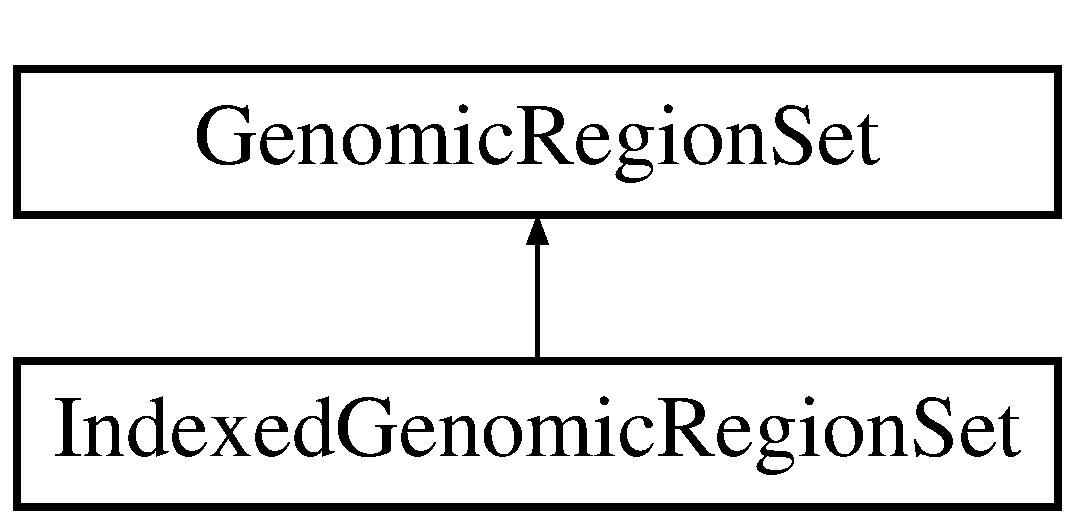
\includegraphics[height=2cm]{classGenomicRegionSet}
\end{center}
\end{figure}
\subsection*{Public Member Functions}
\begin{CompactItemize}
\item 
\hypertarget{classGenomicRegionSet_afc417b2a9a27f3ad833828be5720e92}{
\hyperlink{classGenomicRegionSet_afc417b2a9a27f3ad833828be5720e92}{GenomicRegionSet} (char $\ast$\hyperlink{classGenomicRegionSet_7c593d1beab775590d5b810097644583}{file}, unsigned long int \hyperlink{classGenomicRegionSet_4d60b5403d2d6aaeda541ed45625b245}{buffer\_\-size}, bool \hyperlink{classGenomicRegionSet_2646e9e6d5da1693b4bea36a5acc082e}{verbose}, bool \hyperlink{classGenomicRegionSet_de43c6cd72b95da75395129b00a52687}{load\_\-in\_\-memory}=true)}
\label{classGenomicRegionSet_afc417b2a9a27f3ad833828be5720e92}

\begin{CompactList}\small\item\em Class constructor, see example below. \item\end{CompactList}\item 
\hypertarget{classGenomicRegionSet_8d18f09bd536bae9f2a2494d4cc19f65}{
\hyperlink{classGenomicRegionSet_8d18f09bd536bae9f2a2494d4cc19f65}{GenomicRegionSet} (FILE $\ast$\hyperlink{classGenomicRegionSet_4ca6c6268e39fdea2add6e6381c66962}{file\_\-ptr}, unsigned long int \hyperlink{classGenomicRegionSet_4d60b5403d2d6aaeda541ed45625b245}{buffer\_\-size}, bool \hyperlink{classGenomicRegionSet_2646e9e6d5da1693b4bea36a5acc082e}{verbose}, bool \hyperlink{classGenomicRegionSet_de43c6cd72b95da75395129b00a52687}{load\_\-in\_\-memory}=true)}
\label{classGenomicRegionSet_8d18f09bd536bae9f2a2494d4cc19f65}

\begin{CompactList}\small\item\em Class constructor, see example below. \item\end{CompactList}\item 
\hypertarget{classGenomicRegionSet_3fc7c6dc31cffcedf97a7b69a7f3c2c8}{
virtual \hyperlink{classGenomicRegionSet_3fc7c6dc31cffcedf97a7b69a7f3c2c8}{$\sim$GenomicRegionSet} ()}
\label{classGenomicRegionSet_3fc7c6dc31cffcedf97a7b69a7f3c2c8}

\begin{CompactList}\small\item\em Class destructor. \item\end{CompactList}\item 
\hypertarget{classGenomicRegionSet_6992ccc0c4dd8be0ad4be9b991ab9f36}{
void \hyperlink{classGenomicRegionSet_6992ccc0c4dd8be0ad4be9b991ab9f36}{ProcessFileHeader} (bool hide)}
\label{classGenomicRegionSet_6992ccc0c4dd8be0ad4be9b991ab9f36}

\begin{CompactList}\small\item\em Processes file header. \item\end{CompactList}\item 
\hypertarget{classGenomicRegionSet_5721a1d9ca4ca18ddbcad1e563d42019}{
void \hyperlink{classGenomicRegionSet_5721a1d9ca4ca18ddbcad1e563d42019}{DetectFileFormat} ()}
\label{classGenomicRegionSet_5721a1d9ca4ca18ddbcad1e563d42019}

\begin{CompactList}\small\item\em Detects input format. \item\end{CompactList}\item 
\hypertarget{classGenomicRegionSet_4e8e101aebcedd6a5892d463fe830450}{
\hyperlink{classGenomicRegion}{GenomicRegion} $\ast$ \hyperlink{classGenomicRegionSet_4e8e101aebcedd6a5892d463fe830450}{CreateGenomicRegion} (\hyperlink{classFileBuffer}{FileBuffer} $\ast$\hyperlink{classGenomicRegionSet_df3a5598e31ddbb5b381125925362085}{buffer})}
\label{classGenomicRegionSet_4e8e101aebcedd6a5892d463fe830450}

\begin{CompactList}\small\item\em Creates new genomic region based on input format. \item\end{CompactList}\item 
\hypertarget{classGenomicRegionSet_94b1955e7a4127efaceba25429af7568}{
void \hyperlink{classGenomicRegionSet_94b1955e7a4127efaceba25429af7568}{Init} ()}
\label{classGenomicRegionSet_94b1955e7a4127efaceba25429af7568}

\begin{CompactList}\small\item\em Initializes data structures. \item\end{CompactList}\item 
\hypertarget{classGenomicRegionSet_ae7295913424148013df6a154c5458aa}{
void \hyperlink{classGenomicRegionSet_ae7295913424148013df6a154c5458aa}{Reset} ()}
\label{classGenomicRegionSet_ae7295913424148013df6a154c5458aa}

\begin{CompactList}\small\item\em Resets file; note, that this is not possible if the regions are being read from the standard input. \item\end{CompactList}\item 
\hypertarget{classGenomicRegionSet_06e2e8f91623c01e6e00500888b9ba3d}{
\hyperlink{classGenomicRegion}{GenomicRegion} $\ast$ \hyperlink{classGenomicRegionSet_06e2e8f91623c01e6e00500888b9ba3d}{Begin} ()}
\label{classGenomicRegionSet_06e2e8f91623c01e6e00500888b9ba3d}

\begin{CompactList}\small\item\em Returns pointer to the first region in the set; note, that this is not possible if the regions are being read from the standard input. \item\end{CompactList}\item 
\hypertarget{classGenomicRegionSet_77031066d2648c8935c291ef227b37be}{
virtual \hyperlink{classGenomicRegion}{GenomicRegion} $\ast$ \hyperlink{classGenomicRegionSet_77031066d2648c8935c291ef227b37be}{Get} ()}
\label{classGenomicRegionSet_77031066d2648c8935c291ef227b37be}

\begin{CompactList}\small\item\em Returns pointer to current region in the set. \item\end{CompactList}\item 
\hypertarget{classGenomicRegionSet_4f7501a27d13cae65247686182b78d51}{
virtual \hyperlink{classGenomicRegion}{GenomicRegion} $\ast$ \hyperlink{classGenomicRegionSet_4f7501a27d13cae65247686182b78d51}{Next} ()}
\label{classGenomicRegionSet_4f7501a27d13cae65247686182b78d51}

\begin{CompactList}\small\item\em Moves pointer to next region in the set; if \hyperlink{classGenomicRegionSet_de43c6cd72b95da75395129b00a52687}{GenomicRegionSet::load\_\-in\_\-memory} is 'false', it deletes the current region. \item\end{CompactList}\item 
\hyperlink{classGenomicRegion}{GenomicRegion} $\ast$ \hyperlink{classGenomicRegionSet_c11134b4ccc2ad002ef20ac12d3b70b8}{Next} (bool sorted\_\-by\_\-strand, bool retain\_\-current=false)
\begin{CompactList}\small\item\em Same as \hyperlink{classGenomicRegionSet_4f7501a27d13cae65247686182b78d51}{Next()} but allows user to check sort order and/or retain the current region into memory. \item\end{CompactList}\item 
\hypertarget{classGenomicRegionSet_8993c741ef2513ba5c5b88eb390f1f99}{
void \hyperlink{classGenomicRegionSet_8993c741ef2513ba5c5b88eb390f1f99}{Release} (\hyperlink{classGenomicRegion}{GenomicRegion} $\ast$r)}
\label{classGenomicRegionSet_8993c741ef2513ba5c5b88eb390f1f99}

\begin{CompactList}\small\item\em Deletes genomic region from memory. \item\end{CompactList}\item 
\hypertarget{classGenomicRegionSet_d7dfea15eb8968d376771d74e042f3a1}{
\hyperlink{classGenomicRegion}{GenomicRegion} $\ast$ \hyperlink{classGenomicRegionSet_d7dfea15eb8968d376771d74e042f3a1}{GetRetain} ()}
\label{classGenomicRegionSet_d7dfea15eb8968d376771d74e042f3a1}

\begin{CompactList}\small\item\em \mbox{[}DEPRECATED\mbox{]} Returns current region, and protects its from deletion by \hyperlink{classGenomicRegionSet_4f7501a27d13cae65247686182b78d51}{GenomicRegionSet::Next()}. \item\end{CompactList}\item 
\hypertarget{classGenomicRegionSet_39c746333affb32acffbf0f31b7f6fcf}{
void \hyperlink{classGenomicRegionSet_39c746333affb32acffbf0f31b7f6fcf}{PrintError} (string error\_\-msg)}
\label{classGenomicRegionSet_39c746333affb32acffbf0f31b7f6fcf}

\begin{CompactList}\small\item\em Prints error message. \item\end{CompactList}\item 
\hypertarget{classGenomicRegionSet_260acb32612d31325099c9e53366c9d2}{
long int \hyperlink{classGenomicRegionSet_260acb32612d31325099c9e53366c9d2}{CountRegions} (bool use\_\-label\_\-counts)}
\label{classGenomicRegionSet_260acb32612d31325099c9e53366c9d2}

\begin{CompactList}\small\item\em Counts the number of regions in the set. If {\bf use\_\-label\_\-counts}, the region labels are assumed to be numbers, and the sum of these numbers is reported. \item\end{CompactList}\item 
\hypertarget{classGenomicRegionSet_78c6f4879ac131e6db2094f21b466a98}{
void \hyperlink{classGenomicRegionSet_78c6f4879ac131e6db2094f21b466a98}{RunGlobalAnnotate} (StringLIntMap $\ast$bounds)}
\label{classGenomicRegionSet_78c6f4879ac131e6db2094f21b466a98}

\begin{CompactList}\small\item\em Annotate input region neighborhoods as upstream, downstream, etc. \item\end{CompactList}\item 
\hypertarget{classGenomicRegionSet_619b51265f7bf5d6c92144de689ca8a2}{
void \hyperlink{classGenomicRegionSet_619b51265f7bf5d6c92144de689ca8a2}{RunGlobalCluster} (bool merge=false)}
\label{classGenomicRegionSet_619b51265f7bf5d6c92144de689ca8a2}

\begin{CompactList}\small\item\em Cluster input regions based on pair-wise overlaps (note that this is computationally intensive). \item\end{CompactList}\item 
\hypertarget{classGenomicRegionSet_3d550572975732566378797ac1d8119b}{
void \hyperlink{classGenomicRegionSet_3d550572975732566378797ac1d8119b}{RunGlobalCalcDistances} (char $\ast$op1, char $\ast$op2)}
\label{classGenomicRegionSet_3d550572975732566378797ac1d8119b}

\begin{CompactList}\small\item\em Print distance between successive regions. \item\end{CompactList}\item 
\hypertarget{classGenomicRegionSet_2d6dc99608a1d4938b421fa5a85f5477}{
void \hyperlink{classGenomicRegionSet_2d6dc99608a1d4938b421fa5a85f5477}{RunGlobalSort} ()}
\label{classGenomicRegionSet_2d6dc99608a1d4938b421fa5a85f5477}

\begin{CompactList}\small\item\em Prints sorted region set. \item\end{CompactList}\item 
\hypertarget{classGenomicRegionSet_1056659ccda2e39febb6b87d858a88c4}{
void \hyperlink{classGenomicRegionSet_1056659ccda2e39febb6b87d858a88c4}{RunGlobalInvert} (StringLIntMap $\ast$bounds)}
\label{classGenomicRegionSet_1056659ccda2e39febb6b87d858a88c4}

\begin{CompactList}\small\item\em Prints the difference between chromosome intervals and input region set (input region set must be sorted). \item\end{CompactList}\item 
\hypertarget{classGenomicRegionSet_b9783fb4fead289c7fe107f9bec1865b}{
void \hyperlink{classGenomicRegionSet_b9783fb4fead289c7fe107f9bec1865b}{RunGlobalLink} (bool sorted\_\-by\_\-strand, long int max\_\-difference)}
\label{classGenomicRegionSet_b9783fb4fead289c7fe107f9bec1865b}

\begin{CompactList}\small\item\em Links successive regions if they overlap (input region set must be sorted). \item\end{CompactList}\item 
\hypertarget{classGenomicRegionSet_40dd79548f9d0333f1169bd17a6e9465}{
void \hyperlink{classGenomicRegionSet_40dd79548f9d0333f1169bd17a6e9465}{RunGlobalPartition} ()}
\label{classGenomicRegionSet_40dd79548f9d0333f1169bd17a6e9465}

\begin{CompactList}\small\item\em Partitions overlapping regions into a non-overlapping region set (input region set must be sorted). \item\end{CompactList}\item 
\hypertarget{classGenomicRegionSet_83853c6af4b779a37de284751d09348d}{
void \hyperlink{classGenomicRegionSet_83853c6af4b779a37de284751d09348d}{RunGlobalTest} (bool sorted\_\-by\_\-strand)}
\label{classGenomicRegionSet_83853c6af4b779a37de284751d09348d}

\begin{CompactList}\small\item\em Tests if input region set is sorted. \item\end{CompactList}\item 
\hypertarget{classGenomicRegionSet_53885e10c5dc9aa51ebece77dae63313}{
void \hyperlink{classGenomicRegionSet_53885e10c5dc9aa51ebece77dae63313}{RunGlobalMerge} (long int merge\_\-win)}
\label{classGenomicRegionSet_53885e10c5dc9aa51ebece77dae63313}

\begin{CompactList}\small\item\em Merges successive regions if they are separated by a distance of {\bf merge\_\-win} or less (input region set must be sorted). \item\end{CompactList}\item 
\hypertarget{classGenomicRegionSet_962bb1b26543df14b324d7ab4dd8e404}{
void \hyperlink{classGenomicRegionSet_962bb1b26543df14b324d7ab4dd8e404}{RunGlobalReverseOrder} ()}
\label{classGenomicRegionSet_962bb1b26543df14b324d7ab4dd8e404}

\begin{CompactList}\small\item\em Reverses the order of reverse-strand regions (for this operation, the entire region set must be loaded in memory). \item\end{CompactList}\item 
\hypertarget{classGenomicRegionSet_b8abdbc3c1f4530dc1992fb0766ba5a4}{
void \hyperlink{classGenomicRegionSet_b8abdbc3c1f4530dc1992fb0766ba5a4}{PrintDensities} (\hyperlink{classGenomicRegionSet}{GenomicRegionSet} \&Index, bool report\_\-exact\_\-boundaries)}
\label{classGenomicRegionSet_b8abdbc3c1f4530dc1992fb0766ba5a4}

\begin{CompactList}\small\item\em Computes densities of input regions in index regions in {\bf Index}. This is OBSOLETE, use class \hyperlink{classGenomicRegionSetOverlapScanner}{GenomicRegionSetOverlapScanner} instead. \item\end{CompactList}\item 
\hypertarget{classGenomicRegionSet_14610521cc47631b1459c2e3488b0eec}{
void \hyperlink{classGenomicRegionSet_14610521cc47631b1459c2e3488b0eec}{RunGlobalScan} (StringLIntMap $\ast$bounds, long int win\_\-step, long int win\_\-size)}
\label{classGenomicRegionSet_14610521cc47631b1459c2e3488b0eec}

\begin{CompactList}\small\item\em Scans input regions in sliding windows and reports count distribution (input regions must be sorted). \item\end{CompactList}\item 
void \hyperlink{classGenomicRegionSet_45cac26bedec4d983127b93d2096f735}{RunGlobalScanCount} (StringLIntMap $\ast$bounds, char $\ast$ref\_\-reg\_\-file, long int win\_\-step, long int win\_\-size, bool ignore\_\-reverse\_\-strand, char preprocess, bool use\_\-labels\_\-as\_\-values, long int min\_\-reads)
\begin{CompactList}\small\item\em Scans input regions in sliding windows (input regions must be sorted). See also class \hyperlink{classGenomicRegionSetScanner}{GenomicRegionSetScanner}. \item\end{CompactList}\item 
\hypertarget{classGenomicRegionSet_6377c10b1e9903ff5ae3b0ff9fe20e4d}{
void \hyperlink{classGenomicRegionSet_6377c10b1e9903ff5ae3b0ff9fe20e4d}{RunConvertToWIG} (char $\ast$title, char $\ast$color, char $\ast$position, char $\ast$options, long int span, bool convert\_\-chromosome)}
\label{classGenomicRegionSet_6377c10b1e9903ff5ae3b0ff9fe20e4d}

\begin{CompactList}\small\item\em Prints in Wiggle format. If {\bf convert\_\-chromosome} is 'true', then convert from ENSEMBL to UCSC names (by adding 'chr' prefix to each chromosome name, and by converting 'MT' to 'chrM'). \item\end{CompactList}\item 
\hypertarget{classGenomicRegionSet_da3da7ef918c09867341cda32881d63e}{
void \hyperlink{classGenomicRegionSet_da3da7ef918c09867341cda32881d63e}{RunAlign} (\hyperlink{classChromosomes}{Chromosomes} $\ast$C)}
\label{classGenomicRegionSet_da3da7ef918c09867341cda32881d63e}

\begin{CompactList}\small\item\em Prints alignments of input sequences to reference genome. \item\end{CompactList}\item 
\hypertarget{classGenomicRegionSet_18669fb4dfdf1287aaf9cfceb8329cb5}{
void \hyperlink{classGenomicRegionSet_18669fb4dfdf1287aaf9cfceb8329cb5}{RunConvertToBED} (char $\ast$title, char $\ast$color, char $\ast$position, bool convert\_\-chromosome)}
\label{classGenomicRegionSet_18669fb4dfdf1287aaf9cfceb8329cb5}

\begin{CompactList}\small\item\em Converts to BED format. If {\bf convert\_\-chromosome} is 'true', then convert from ENSEMBL to UCSC names (by adding 'chr' prefix to each chromosome name, and by converting 'MT' to 'chrM'). \item\end{CompactList}\item 
\hypertarget{classGenomicRegionSet_d7ad039dd702837f37c2cdfebd9b2845}{
void \hyperlink{classGenomicRegionSet_d7ad039dd702837f37c2cdfebd9b2845}{RunBounds} (StringLIntMap $\ast$bounds)}
\label{classGenomicRegionSet_d7ad039dd702837f37c2cdfebd9b2845}

\begin{CompactList}\small\item\em Corrects interval start/stop positions so as to comply with chromosomal bounds. \item\end{CompactList}\item 
\hypertarget{classGenomicRegionSet_1aa8f41f0978e9b66c6f11c0ccb95a0b}{
void \hyperlink{classGenomicRegionSet_1aa8f41f0978e9b66c6f11c0ccb95a0b}{RunCenter} ()}
\label{classGenomicRegionSet_1aa8f41f0978e9b66c6f11c0ccb95a0b}

\begin{CompactList}\small\item\em Print intervals' center. \item\end{CompactList}\item 
\hypertarget{classGenomicRegionSet_752b7d4d2ac3568e7bdb13edbfc00af3}{
void \hyperlink{classGenomicRegionSet_752b7d4d2ac3568e7bdb13edbfc00af3}{RunConnect} ()}
\label{classGenomicRegionSet_752b7d4d2ac3568e7bdb13edbfc00af3}

\begin{CompactList}\small\item\em Print connected intervals as a single interval from minimum start to maximum stop position. \item\end{CompactList}\item 
\hypertarget{classGenomicRegionSet_90256738bd85501460874ab8e69b894b}{
void \hyperlink{classGenomicRegionSet_90256738bd85501460874ab8e69b894b}{RunDiff} ()}
\label{classGenomicRegionSet_90256738bd85501460874ab8e69b894b}

\begin{CompactList}\small\item\em Print gap intervals between successive intervals (e.g. for computing intron boundaries). \item\end{CompactList}\item 
\hypertarget{classGenomicRegionSet_22f3fce9421a0f80c96ec0a9346fec19}{
void \hyperlink{classGenomicRegionSet_22f3fce9421a0f80c96ec0a9346fec19}{RunCalcDistances} (char $\ast$op1, char $\ast$op2)}
\label{classGenomicRegionSet_22f3fce9421a0f80c96ec0a9346fec19}

\begin{CompactList}\small\item\em Print distances between successive intervals of each region (i.e. local operation). \item\end{CompactList}\item 
\hypertarget{classGenomicRegionSet_9acb3424739ed62c0efddad01536ad18}{
void \hyperlink{classGenomicRegionSet_9acb3424739ed62c0efddad01536ad18}{RunDivide} ()}
\label{classGenomicRegionSet_9acb3424739ed62c0efddad01536ad18}

\begin{CompactList}\small\item\em Print intervals divided in half (i.e. two intervals for each original interval in the genomic region). \item\end{CompactList}\item 
\hypertarget{classGenomicRegionSet_efa09dc62c768a06e4ca1f56fd683be5}{
void \hyperlink{classGenomicRegionSet_efa09dc62c768a06e4ca1f56fd683be5}{RunFix} ()}
\label{classGenomicRegionSet_efa09dc62c768a06e4ca1f56fd683be5}

\begin{CompactList}\small\item\em Removes rogue intervals (e.g. start$>$stop). \item\end{CompactList}\item 
\hypertarget{classGenomicRegionSet_e598cd9c5f94555a04e43f9fe6334aec}{
void \hyperlink{classGenomicRegionSet_e598cd9c5f94555a04e43f9fe6334aec}{RunIntersection} ()}
\label{classGenomicRegionSet_e598cd9c5f94555a04e43f9fe6334aec}

\begin{CompactList}\small\item\em Print intersection among all intervals, i.e. maximum start to minimum stop position. \item\end{CompactList}\item 
\hypertarget{classGenomicRegionSet_b1e96bd7781dac63a1745a8cf5ac5538}{
void \hyperlink{classGenomicRegionSet_b1e96bd7781dac63a1745a8cf5ac5538}{RunSize} ()}
\label{classGenomicRegionSet_b1e96bd7781dac63a1745a8cf5ac5538}

\begin{CompactList}\small\item\em Prints region label and sum of intervals' sizes. \item\end{CompactList}\item 
void \hyperlink{classGenomicRegionSet_11f1e58c92e9b0b2e3feb5821cff1a55}{RunModifyPos} (char $\ast$position\_\-op, long int position\_\-shift)
\begin{CompactList}\small\item\em Modifies interval start/stop positions. First it chooses which position to keep fixed, and then it shifts the non-fixed position. \item\end{CompactList}\item 
\hypertarget{classGenomicRegionSet_8f71dd5fa48a0878751cd78a3b485daf}{
void \hyperlink{classGenomicRegionSet_8f71dd5fa48a0878751cd78a3b485daf}{RunConvertToREG} (bool compact=false)}
\label{classGenomicRegionSet_8f71dd5fa48a0878751cd78a3b485daf}

\begin{CompactList}\small\item\em Prints label and genomic region intervals with a newline character at the end for all regions in the set. \item\end{CompactList}\item 
\hypertarget{classGenomicRegionSet_1b2b9edad211ca961f319921d38bfbf6}{
void \hyperlink{classGenomicRegionSet_1b2b9edad211ca961f319921d38bfbf6}{RunRandomize} (gsl\_\-rng $\ast$random\_\-generator, StringLIntMap $\ast$bounds)}
\label{classGenomicRegionSet_1b2b9edad211ca961f319921d38bfbf6}

\begin{CompactList}\small\item\em Randomizes interval position within chromosomal bounds. \item\end{CompactList}\item 
\hypertarget{classGenomicRegionSet_7b522944fe4f7f489c99fb76ce7f576c}{
void \hyperlink{classGenomicRegionSet_7b522944fe4f7f489c99fb76ce7f576c}{RunSelect} (bool first, bool last, bool from5p, bool from3p)}
\label{classGenomicRegionSet_7b522944fe4f7f489c99fb76ce7f576c}

\begin{CompactList}\small\item\em Selects a subset of intervals according to their relative positions. \item\end{CompactList}\item 
void \hyperlink{classGenomicRegionSet_d4b42becffb21de5e89129476c79c851}{RunShiftPos} (long int start\_\-shift, long int stop\_\-shift, bool shift\_\-5prime)
\begin{CompactList}\small\item\em Shifts interval start/stop positions. First it chooses reference position, and then shifts start and stop positions separately. \item\end{CompactList}\item 
\hypertarget{classGenomicRegionSet_53143cb3271c65fb289faece622cd8bd}{
void \hyperlink{classGenomicRegionSet_53143cb3271c65fb289faece622cd8bd}{RunSort} ()}
\label{classGenomicRegionSet_53143cb3271c65fb289faece622cd8bd}

\begin{CompactList}\small\item\em Print sorted intervals according to start position (only for compatible intervals). \item\end{CompactList}\item 
\hypertarget{classGenomicRegionSet_570e56362af1b30e7f5cb149ea42e54e}{
void \hyperlink{classGenomicRegionSet_570e56362af1b30e7f5cb149ea42e54e}{RunSplit} ()}
\label{classGenomicRegionSet_570e56362af1b30e7f5cb149ea42e54e}

\begin{CompactList}\small\item\em Split regions into intervals which are printed on separate lines. \item\end{CompactList}\item 
\hypertarget{classGenomicRegionSet_f1146729843b82d7637e0adc1b07e51a}{
void \hyperlink{classGenomicRegionSet_f1146729843b82d7637e0adc1b07e51a}{RunModifyStrand} (char $\ast$strand\_\-op, bool sorted)}
\label{classGenomicRegionSet_f1146729843b82d7637e0adc1b07e51a}

\begin{CompactList}\small\item\em Print region with modified strands: '+'=only forward, '-'=only reverse, 'r'=reverse strands from '+' to '-' and vice versa; if {\bf sorted} is 'true', it calls \hyperlink{classGenomicRegionSet_7c0a328896b88a0c837f60e89fd85584}{GenomicRegionSet::RunModifyStrandSorted} instead. \item\end{CompactList}\item 
\hypertarget{classGenomicRegionSet_7c0a328896b88a0c837f60e89fd85584}{
void \hyperlink{classGenomicRegionSet_7c0a328896b88a0c837f60e89fd85584}{RunModifyStrandSorted} (char $\ast$strand\_\-op)}
\label{classGenomicRegionSet_7c0a328896b88a0c837f60e89fd85584}

\begin{CompactList}\small\item\em Same as \hyperlink{classGenomicRegionSet_f1146729843b82d7637e0adc1b07e51a}{GenomicRegionSet::RunModifyStrand} but returns a sorted region set (note: it only works if the original region set is sorted). \item\end{CompactList}\item 
\hypertarget{classGenomicRegionSet_015049fd0bd08587cbdbb49332ee352d}{
void \hyperlink{classGenomicRegionSet_015049fd0bd08587cbdbb49332ee352d}{RunShuffle} (gsl\_\-rng $\ast$random\_\-generator, char $\ast$ref\_\-reg\_\-file)}
\label{classGenomicRegionSet_015049fd0bd08587cbdbb49332ee352d}

\begin{CompactList}\small\item\em Shuffles input regions within specified reference regions loaded from file {\bf ref\_\-reg\_\-file}. \item\end{CompactList}\item 
\hypertarget{classGenomicRegionSet_b281c8ab57c4181a06161182031c9df4}{
void \hyperlink{classGenomicRegionSet_b281c8ab57c4181a06161182031c9df4}{RunUnion} ()}
\label{classGenomicRegionSet_b281c8ab57c4181a06161182031c9df4}

\begin{CompactList}\small\item\em Print intervals' union. \item\end{CompactList}\item 
\hypertarget{classGenomicRegionSet_a326d5adcc97f47ed2de35353b60b393}{
void \hyperlink{classGenomicRegionSet_a326d5adcc97f47ed2de35353b60b393}{RunSlidingWindows} (long int win\_\-step, long int win\_\-size)}
\label{classGenomicRegionSet_a326d5adcc97f47ed2de35353b60b393}

\begin{CompactList}\small\item\em Print sliding windows (implemented only for single-interval regions). \item\end{CompactList}\item 
\hypertarget{classGenomicRegionSet_b219b834c232c091982b066a2163f76a}{
void \hyperlink{classGenomicRegionSet_b219b834c232c091982b066a2163f76a}{RunExtractSeq} (\hyperlink{classChromosomes}{Chromosomes} $\ast$C, bool replace=false)}
\label{classGenomicRegionSet_b219b834c232c091982b066a2163f76a}

\begin{CompactList}\small\item\em Prints region label, intervals and extracted sequence in SEQ format. \item\end{CompactList}\item 
\hypertarget{classGenomicRegionSet_de00553eb76b71f68e540739bdc776f4}{
void \hyperlink{classGenomicRegionSet_de00553eb76b71f68e540739bdc776f4}{PrintBEDGraphFormat} (char $\ast$title, char $\ast$color, char $\ast$position, bool convert\_\-chromosome)}
\label{classGenomicRegionSet_de00553eb76b71f68e540739bdc776f4}

\begin{CompactList}\small\item\em Prints in BEDGraph format. If {\bf convert\_\-chromosome} is 'true', then convert from ENSEMBL to UCSC names (by adding 'chr' prefix to each chromosome name, and by converting 'MT' to 'chrM'). \item\end{CompactList}\item 
\hypertarget{classGenomicRegionSet_3da972129b9b69577bbe0bb9837bbea3}{
void \hyperlink{classGenomicRegionSet_3da972129b9b69577bbe0bb9837bbea3}{PrintSeqLength} (\hyperlink{classChromosomes}{Chromosomes} $\ast$C)}
\label{classGenomicRegionSet_3da972129b9b69577bbe0bb9837bbea3}

\begin{CompactList}\small\item\em Prints region label and sequence length excluding 'N' characters. \item\end{CompactList}\item 
void \hyperlink{classGenomicRegionSet_6dc7150acdd7a0614f8a8497da687d0e}{PrintRemoveN} (\hyperlink{classChromosomes}{Chromosomes} $\ast$C)
\begin{CompactList}\small\item\em Print sequence with no alignment gaps (requires SEQ input). \item\end{CompactList}\item 
void \hyperlink{classGenomicRegionSet_e27a5c9f17f08afae277603e33d4fb91}{PrintOffsetFormat} (char $\ast$op, bool fraction)
\begin{CompactList}\small\item\em Calculates the offset distances of interval start and stop position with respect to the first interval in the set. \item\end{CompactList}\item 
\hypertarget{classGenomicRegionSet_c8de83151ba0cc30ca1b72e83ecea82f}{
void \hyperlink{classGenomicRegionSet_c8de83151ba0cc30ca1b72e83ecea82f}{PrintReversePos} (StringLIntMap $\ast$bounds)}
\label{classGenomicRegionSet_c8de83151ba0cc30ca1b72e83ecea82f}

\begin{CompactList}\small\item\em Reverses interval start/stop positions with respect to chromosomal bounds, as if the reference point were in the end of the chromosome as opposed to the beginning. \item\end{CompactList}\item 
\hypertarget{classGenomicRegionSet_dfbad7f0acf42c2179bd33103e5d183c}{
void \hyperlink{classGenomicRegionSet_dfbad7f0acf42c2179bd33103e5d183c}{PrintSearch} (char $\ast$pattern, bool header, bool summary)}
\label{classGenomicRegionSet_dfbad7f0acf42c2179bd33103e5d183c}

\begin{CompactList}\small\item\em Search sequence for short pattern (requires SEQ input). \item\end{CompactList}\item 
\hypertarget{classGenomicRegionSet_4c197a09ffcace2ec2736aa089eec448}{
void \hyperlink{classGenomicRegionSet_4c197a09ffcace2ec2736aa089eec448}{PrintVerifySeq} (\hyperlink{classChromosomes}{Chromosomes} $\ast$C, bool ignore)}
\label{classGenomicRegionSet_4c197a09ffcace2ec2736aa089eec448}

\begin{CompactList}\small\item\em Verifies extracted sequence against region label. \item\end{CompactList}\end{CompactItemize}
\subsection*{Public Attributes}
\begin{CompactItemize}
\item 
\hypertarget{classGenomicRegionSet_7c593d1beab775590d5b810097644583}{
char $\ast$ \hyperlink{classGenomicRegionSet_7c593d1beab775590d5b810097644583}{file}}
\label{classGenomicRegionSet_7c593d1beab775590d5b810097644583}

\begin{CompactList}\small\item\em file name ('NULL' if reading from standard input) \item\end{CompactList}\item 
\hypertarget{classGenomicRegionSet_4ca6c6268e39fdea2add6e6381c66962}{
FILE $\ast$ \hyperlink{classGenomicRegionSet_4ca6c6268e39fdea2add6e6381c66962}{file\_\-ptr}}
\label{classGenomicRegionSet_4ca6c6268e39fdea2add6e6381c66962}

\begin{CompactList}\small\item\em file pointer ('NULL' if reading from standard input) \item\end{CompactList}\item 
\hypertarget{classGenomicRegionSet_4d60b5403d2d6aaeda541ed45625b245}{
unsigned long int \hyperlink{classGenomicRegionSet_4d60b5403d2d6aaeda541ed45625b245}{buffer\_\-size}}
\label{classGenomicRegionSet_4d60b5403d2d6aaeda541ed45625b245}

\begin{CompactList}\small\item\em line buffer size (automatically adjusted during execution to ensure the entire line is read) \item\end{CompactList}\item 
\hypertarget{classGenomicRegionSet_2646e9e6d5da1693b4bea36a5acc082e}{
bool \hyperlink{classGenomicRegionSet_2646e9e6d5da1693b4bea36a5acc082e}{verbose}}
\label{classGenomicRegionSet_2646e9e6d5da1693b4bea36a5acc082e}

\begin{CompactList}\small\item\em verbose mode \item\end{CompactList}\item 
\hypertarget{classGenomicRegionSet_bd0fc2542e717e5855e03d3b3892f027}{
bool \hyperlink{classGenomicRegionSet_bd0fc2542e717e5855e03d3b3892f027}{from\_\-stdin}}
\label{classGenomicRegionSet_bd0fc2542e717e5855e03d3b3892f027}

\begin{CompactList}\small\item\em 'true' if reading from standard input \item\end{CompactList}\item 
\hypertarget{classGenomicRegionSet_de43c6cd72b95da75395129b00a52687}{
bool \hyperlink{classGenomicRegionSet_de43c6cd72b95da75395129b00a52687}{load\_\-in\_\-memory}}
\label{classGenomicRegionSet_de43c6cd72b95da75395129b00a52687}

\begin{CompactList}\small\item\em 'true' if the entire region set is loaded in memory \item\end{CompactList}\item 
\hypertarget{classGenomicRegionSet_ea8b5c9bae036da50d4e8720d2e13231}{
bool \hyperlink{classGenomicRegionSet_ea8b5c9bae036da50d4e8720d2e13231}{use\_\-interval\_\-array}}
\label{classGenomicRegionSet_ea8b5c9bae036da50d4e8720d2e13231}

\begin{CompactList}\small\item\em if 'true' use an array for storing genomic regions' intervals (for time efficiency) \item\end{CompactList}\item 
\hypertarget{classGenomicRegionSet_a4494ed2ae3f7594c29b18c39fed6748}{
string \hyperlink{classGenomicRegionSet_a4494ed2ae3f7594c29b18c39fed6748}{format}}
\label{classGenomicRegionSet_a4494ed2ae3f7594c29b18c39fed6748}

\begin{CompactList}\small\item\em input format \item\end{CompactList}\item 
\hypertarget{classGenomicRegionSet_08d9a35a7688ac2c193b53c9a8693c6e}{
\hyperlink{classProgress}{Progress} \hyperlink{classGenomicRegionSet_08d9a35a7688ac2c193b53c9a8693c6e}{progress}}
\label{classGenomicRegionSet_08d9a35a7688ac2c193b53c9a8693c6e}

\begin{CompactList}\small\item\em keeps track of progress of computation \item\end{CompactList}\item 
\hypertarget{classGenomicRegionSet_df3a5598e31ddbb5b381125925362085}{
\hyperlink{classFileBuffer}{FileBuffer} $\ast$ \hyperlink{classGenomicRegionSet_df3a5598e31ddbb5b381125925362085}{buffer}}
\label{classGenomicRegionSet_df3a5598e31ddbb5b381125925362085}

\begin{CompactList}\small\item\em pointer to the buffer class used to read the region sets \item\end{CompactList}\item 
\hypertarget{classGenomicRegionSet_5293292428aa06145b38be4b96ab05e4}{
long int \hyperlink{classGenomicRegionSet_5293292428aa06145b38be4b96ab05e4}{n\_\-regions}}
\label{classGenomicRegionSet_5293292428aa06145b38be4b96ab05e4}

\begin{CompactList}\small\item\em number of regions ('1' if the regions are not loaded in memory) \item\end{CompactList}\item 
\hypertarget{classGenomicRegionSet_206d91b443832800afc04f786d15971d}{
\hyperlink{classGenomicRegion}{GenomicRegion} $\ast$$\ast$ \hyperlink{classGenomicRegionSet_206d91b443832800afc04f786d15971d}{R}}
\label{classGenomicRegionSet_206d91b443832800afc04f786d15971d}

\begin{CompactList}\small\item\em array where the regions are stored; if the region set is not entirely loaded in memory, only {\bf R\mbox{[}0\mbox{]}} is used \item\end{CompactList}\item 
\hypertarget{classGenomicRegionSet_d89185b88d5b37161cc65bc84b421c0e}{
long int \hyperlink{classGenomicRegionSet_d89185b88d5b37161cc65bc84b421c0e}{r\_\-index}}
\label{classGenomicRegionSet_d89185b88d5b37161cc65bc84b421c0e}

\begin{CompactList}\small\item\em index pointing to the current region in {\bf R} \item\end{CompactList}\end{CompactItemize}
\subsection*{Private Member Functions}
\begin{CompactItemize}
\item 
\hypertarget{classGenomicRegionSet_cd823956ec9f510ee3d52b08eec1b2f6}{
\hyperlink{classGenomicRegionSet}{GenomicRegionSet} $\ast$ \hyperlink{classGenomicRegionSet_cd823956ec9f510ee3d52b08eec1b2f6}{StoreInTempFile} ()}
\label{classGenomicRegionSet_cd823956ec9f510ee3d52b08eec1b2f6}

\begin{CompactList}\small\item\em Creates a temporary file from this instance of \hyperlink{classGenomicRegionSet}{GenomicRegionSet} which contains the current chromosome's positive strand regions (used in \hyperlink{classGenomicRegionSet_7c0a328896b88a0c837f60e89fd85584}{GenomicRegionSet::RunModifyStrandSorted}). \item\end{CompactList}\item 
\hypertarget{classGenomicRegionSet_b118bb8a6b63ae47a37ef89bff25ab72}{
\hyperlink{classGenomicRegion}{GenomicRegion} $\ast$ \hyperlink{classGenomicRegionSet_b118bb8a6b63ae47a37ef89bff25ab72}{PrintMergeSort} (\hyperlink{classGenomicRegionSet}{GenomicRegionSet} $\ast$rtempSet, char strand)}
\label{classGenomicRegionSet_b118bb8a6b63ae47a37ef89bff25ab72}

\begin{CompactList}\small\item\em Uses mergesort between {\bf tempSet} and this instance of \hyperlink{classGenomicRegionSet}{GenomicRegionSet} (used in \hyperlink{classGenomicRegionSet_7c0a328896b88a0c837f60e89fd85584}{GenomicRegionSet::RunModifyStrandSorted}). \item\end{CompactList}\item 
\hypertarget{classGenomicRegionSet_e601878a7754a7e5bc8b4ed340d012f4}{
\hyperlink{classGenomicRegion}{GenomicRegion} $\ast$ \hyperlink{classGenomicRegionSet_e601878a7754a7e5bc8b4ed340d012f4}{PrintReverse} (\hyperlink{classGenomicRegionSet}{GenomicRegionSet} $\ast$rtempSet)}
\label{classGenomicRegionSet_e601878a7754a7e5bc8b4ed340d012f4}

\begin{CompactList}\small\item\em Reverses the order between {\bf tempSet} and this instance of \hyperlink{classGenomicRegionSet}{GenomicRegionSet} (used in \hyperlink{classGenomicRegionSet_7c0a328896b88a0c837f60e89fd85584}{GenomicRegionSet::RunModifyStrandSorted}). \item\end{CompactList}\end{CompactItemize}


\subsection{Detailed Description}
This class is used to read and manipulate a set of genomic regions from a file or from standard input. 

Example: 

\begin{Code}\begin{verbatim}    GenomicRegionSet RegSet("test.reg",10000,true);
    Progress PRG("Printing center of intervals...",1);
    for (GenomicRegion *r=RegSet.Get(); r!=NULL; r=RegSet.Next()) {
      r->Center();
      r->Print();
      PRG.Check();
    }
    PRG.Done();
\end{verbatim}
\end{Code}

 

\subsection{Member Function Documentation}
\hypertarget{classGenomicRegionSet_c11134b4ccc2ad002ef20ac12d3b70b8}{
\index{GenomicRegionSet@{GenomicRegionSet}!Next@{Next}}
\index{Next@{Next}!GenomicRegionSet@{GenomicRegionSet}}
\subsubsection[Next]{\setlength{\rightskip}{0pt plus 5cm}{\bf GenomicRegion} $\ast$ GenomicRegionSet::Next (bool {\em sorted\_\-by\_\-strand}, \/  bool {\em retain\_\-current} = {\tt false})}}
\label{classGenomicRegionSet_c11134b4ccc2ad002ef20ac12d3b70b8}


Same as \hyperlink{classGenomicRegionSet_4f7501a27d13cae65247686182b78d51}{Next()} but allows user to check sort order and/or retain the current region into memory. 

\begin{Desc}
\item[Parameters:]
\begin{description}
\item[{\em sorted\_\-by\_\-strand}]if 'true', it takes into account strand information while checking the sort order \item[{\em retain\_\-current}]if 'true', the current region is not deleted from memory; this must be done 'manually' using the \hyperlink{classGenomicRegionSet_8993c741ef2513ba5c5b88eb390f1f99}{Release()} method (do not use 'delete'). \end{description}
\end{Desc}
\hypertarget{classGenomicRegionSet_45cac26bedec4d983127b93d2096f735}{
\index{GenomicRegionSet@{GenomicRegionSet}!RunGlobalScanCount@{RunGlobalScanCount}}
\index{RunGlobalScanCount@{RunGlobalScanCount}!GenomicRegionSet@{GenomicRegionSet}}
\subsubsection[RunGlobalScanCount]{\setlength{\rightskip}{0pt plus 5cm}void GenomicRegionSet::RunGlobalScanCount (StringLIntMap $\ast$ {\em bounds}, \/  char $\ast$ {\em ref\_\-reg\_\-file}, \/  long int {\em win\_\-step}, \/  long int {\em win\_\-size}, \/  bool {\em ignore\_\-reverse\_\-strand}, \/  char {\em preprocess}, \/  bool {\em use\_\-labels\_\-as\_\-values}, \/  long int {\em min\_\-reads})}}
\label{classGenomicRegionSet_45cac26bedec4d983127b93d2096f735}


Scans input regions in sliding windows (input regions must be sorted). See also class \hyperlink{classGenomicRegionSetScanner}{GenomicRegionSetScanner}. 

\begin{Desc}
\item[Parameters:]
\begin{description}
\item[{\em bounds}]chromosome sizes \item[{\em ref\_\-reg\_\-file}]only windows that overlap with regions in this file will be reported \item[{\em win\_\-step}]sliding window step \item[{\em win\_\-size}]sliding window size (must be a multiple of window step) \item[{\em ignore\_\-reverse\_\-strand}]if true, no sliding windows on the negative strand are reported \item[{\em preprocess}]if '1', only start position is counted; if 'p', all positions are counted; if 'c', center of interval is counted \item[{\em use\_\-labels\_\-as\_\-values}]if true, genomic region labels are assumed to be integers and are included in the counting \item[{\em min\_\-reads}]report windows only if value is greater that this parameter \end{description}
\end{Desc}
\hypertarget{classGenomicRegionSet_11f1e58c92e9b0b2e3feb5821cff1a55}{
\index{GenomicRegionSet@{GenomicRegionSet}!RunModifyPos@{RunModifyPos}}
\index{RunModifyPos@{RunModifyPos}!GenomicRegionSet@{GenomicRegionSet}}
\subsubsection[RunModifyPos]{\setlength{\rightskip}{0pt plus 5cm}void GenomicRegionSet::RunModifyPos (char $\ast$ {\em position\_\-op}, \/  long int {\em position\_\-shift})}}
\label{classGenomicRegionSet_11f1e58c92e9b0b2e3feb5821cff1a55}


Modifies interval start/stop positions. First it chooses which position to keep fixed, and then it shifts the non-fixed position. 

\begin{Desc}
\item[Parameters:]
\begin{description}
\item[{\em position\_\-op}]selects fixed position as follows: '1'=start position, 'c'=center position, '5p'=5-prime, '3p'=3-prime \item[{\em position\_\-shift}]determines the shift of the non-fixed position (in the 'c' case, both positions are shifted symmetrically around the center) \end{description}
\end{Desc}
\hypertarget{classGenomicRegionSet_d4b42becffb21de5e89129476c79c851}{
\index{GenomicRegionSet@{GenomicRegionSet}!RunShiftPos@{RunShiftPos}}
\index{RunShiftPos@{RunShiftPos}!GenomicRegionSet@{GenomicRegionSet}}
\subsubsection[RunShiftPos]{\setlength{\rightskip}{0pt plus 5cm}void GenomicRegionSet::RunShiftPos (long int {\em start\_\-shift}, \/  long int {\em stop\_\-shift}, \/  bool {\em shift\_\-5prime})}}
\label{classGenomicRegionSet_d4b42becffb21de5e89129476c79c851}


Shifts interval start/stop positions. First it chooses reference position, and then shifts start and stop positions separately. 

\begin{Desc}
\item[Parameters:]
\begin{description}
\item[{\em start\_\-shift}]determines the shift of the start position \item[{\em stop\_\-shift}]determines the shift of the stop position \item[{\em shift\_\-5prime}]if 'true', then the new start position is the old 5-prime position shifted by {\bf start\_\-shift} and the new stop position is the old 3-prime position shifted by {\bf stop\_\-shift} \end{description}
\end{Desc}
\hypertarget{classGenomicRegionSet_6dc7150acdd7a0614f8a8497da687d0e}{
\index{GenomicRegionSet@{GenomicRegionSet}!PrintRemoveN@{PrintRemoveN}}
\index{PrintRemoveN@{PrintRemoveN}!GenomicRegionSet@{GenomicRegionSet}}
\subsubsection[PrintRemoveN]{\setlength{\rightskip}{0pt plus 5cm}void GenomicRegionSet::PrintRemoveN ({\bf Chromosomes} $\ast$ {\em C})}}
\label{classGenomicRegionSet_6dc7150acdd7a0614f8a8497da687d0e}


Print sequence with no alignment gaps (requires SEQ input). 

Remove sub-intervals that correspond to sequences of 'N' characters \hypertarget{classGenomicRegionSet_e27a5c9f17f08afae277603e33d4fb91}{
\index{GenomicRegionSet@{GenomicRegionSet}!PrintOffsetFormat@{PrintOffsetFormat}}
\index{PrintOffsetFormat@{PrintOffsetFormat}!GenomicRegionSet@{GenomicRegionSet}}
\subsubsection[PrintOffsetFormat]{\setlength{\rightskip}{0pt plus 5cm}void GenomicRegionSet::PrintOffsetFormat (char $\ast$ {\em op}, \/  bool {\em fraction})}}
\label{classGenomicRegionSet_e27a5c9f17f08afae277603e33d4fb91}


Calculates the offset distances of interval start and stop position with respect to the first interval in the set. 

\begin{Desc}
\item[Parameters:]
\begin{description}
\item[{\em op}]determines reference point as follows: '1'=start position, '2'=stop position, '5p'=5-prime position, '3p'=3-prime position \item[{\em fraction}]if 'true', offsets are reported as a fraction of the total region length \end{description}
\end{Desc}


The documentation for this class was generated from the following files:\begin{CompactItemize}
\item 
genomic\_\-intervals.h\item 
genomic\_\-intervals.cpp\end{CompactItemize}

\hypertarget{classGenomicRegionSetOverlaps}{
\section{GenomicRegionSetOverlaps Class Reference}
\label{classGenomicRegionSetOverlaps}\index{GenomicRegionSetOverlaps@{GenomicRegionSetOverlaps}}
}
Abstract class for computing overlaps between genomic regions.  


{\tt \#include $<$genomic\_\-intervals.h$>$}

Inheritance diagram for GenomicRegionSetOverlaps::\begin{figure}[H]
\begin{center}
\leavevmode
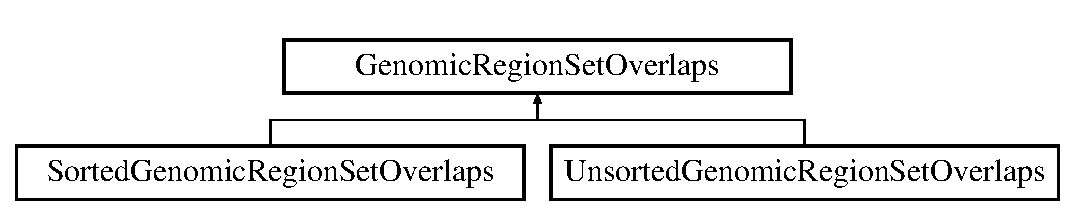
\includegraphics[height=2cm]{classGenomicRegionSetOverlaps}
\end{center}
\end{figure}
\subsection*{Public Member Functions}
\begin{CompactItemize}
\item 
\hyperlink{classGenomicRegionSetOverlaps_67c96149c0881747110db61e76f8c5de}{GenomicRegionSetOverlaps} (\hyperlink{classGenomicRegionSet}{GenomicRegionSet} $\ast$\hyperlink{classGenomicRegionSetOverlaps_e513304379055f6d379bc5907733dbe2}{QuerySet}, \hyperlink{classGenomicRegionSet}{GenomicRegionSet} $\ast$\hyperlink{classGenomicRegionSetOverlaps_c587bf854c827381493735b473622e03}{IndexSet})
\begin{CompactList}\small\item\em Class constructor. \item\end{CompactList}\item 
\hypertarget{classGenomicRegionSetOverlaps_6d9f677e16839c931657c0200b56d99e}{
virtual \hyperlink{classGenomicRegionSetOverlaps_6d9f677e16839c931657c0200b56d99e}{$\sim$GenomicRegionSetOverlaps} ()}
\label{classGenomicRegionSetOverlaps_6d9f677e16839c931657c0200b56d99e}

\begin{CompactList}\small\item\em Class destructor. \item\end{CompactList}\item 
\hypertarget{classGenomicRegionSetOverlaps_709ccfbe8c41154eaf590ca5aa9e12c5}{
virtual \hyperlink{classGenomicRegion}{GenomicRegion} $\ast$ \hyperlink{classGenomicRegionSetOverlaps_709ccfbe8c41154eaf590ca5aa9e12c5}{GetQuery} ()=0}
\label{classGenomicRegionSetOverlaps_709ccfbe8c41154eaf590ca5aa9e12c5}

\begin{CompactList}\small\item\em Returns a pointer to the current query region ('NULL' if no more query regions are available). \item\end{CompactList}\item 
\hypertarget{classGenomicRegionSetOverlaps_21900a952fc925e5bc1840aff106a887}{
virtual \hyperlink{classGenomicRegion}{GenomicRegion} $\ast$ \hyperlink{classGenomicRegionSetOverlaps_21900a952fc925e5bc1840aff106a887}{NextQuery} ()=0}
\label{classGenomicRegionSetOverlaps_21900a952fc925e5bc1840aff106a887}

\begin{CompactList}\small\item\em Returns a pointer to the next query region ('NULL' if no more query regions are available). \item\end{CompactList}\item 
\hypertarget{classGenomicRegionSetOverlaps_e6d1c3bd67b0a902649aab01909a9c10}{
virtual \hyperlink{classGenomicRegion}{GenomicRegion} $\ast$ \hyperlink{classGenomicRegionSetOverlaps_e6d1c3bd67b0a902649aab01909a9c10}{GetMatch} ()=0}
\label{classGenomicRegionSetOverlaps_e6d1c3bd67b0a902649aab01909a9c10}

\begin{CompactList}\small\item\em Returns a pointer to the current index region that overlaps the current query region (even if the overlap is only in the gaps between intervals). \item\end{CompactList}\item 
\hypertarget{classGenomicRegionSetOverlaps_402b8d4c8e9b4499a0612899b0b9ba05}{
virtual \hyperlink{classGenomicRegion}{GenomicRegion} $\ast$ \hyperlink{classGenomicRegionSetOverlaps_402b8d4c8e9b4499a0612899b0b9ba05}{NextMatch} ()=0}
\label{classGenomicRegionSetOverlaps_402b8d4c8e9b4499a0612899b0b9ba05}

\begin{CompactList}\small\item\em Returns a pointer to the next index region that overlaps the current query region (even if the overlap is only in the gaps between intervals). \item\end{CompactList}\item 
\hypertarget{classGenomicRegionSetOverlaps_3371a386fed061f58dbd395aff7afefe}{
virtual bool \hyperlink{classGenomicRegionSetOverlaps_3371a386fed061f58dbd395aff7afefe}{Done} ()=0}
\label{classGenomicRegionSetOverlaps_3371a386fed061f58dbd395aff7afefe}

\begin{CompactList}\small\item\em Returns true, if no more query or index regions are available and the \hyperlink{classSortedGenomicRegionSetOverlaps_19fa18e6abd9f045786698fff48a445f}{SortedGenomicRegionSetOverlaps::IRegBuffer} buffer is empty. \item\end{CompactList}\item 
\hyperlink{classGenomicRegion}{GenomicRegion} $\ast$ \hyperlink{classGenomicRegionSetOverlaps_46c3193d39eb61430b0267ca301b226e}{GetOverlap} (bool match\_\-gaps, bool ignore\_\-strand)
\begin{CompactList}\small\item\em Returns a pointer to the current index region that overlaps the current query region. \item\end{CompactList}\item 
\hyperlink{classGenomicRegion}{GenomicRegion} $\ast$ \hyperlink{classGenomicRegionSetOverlaps_2fa112eab38f07e7bc75ac76f5b9fc67}{NextOverlap} (bool match\_\-gaps, bool ignore\_\-strand)
\begin{CompactList}\small\item\em Returns a pointer to the next index region that overlaps the current query region (even if the overlap is only in the gaps between intervals). \item\end{CompactList}\item 
unsigned long int \hyperlink{classGenomicRegionSetOverlaps_1e30ae0e49423a432b7a1d3e3ff09011}{CalcQueryCoverage} (bool match\_\-gaps, bool ignore\_\-strand, bool use\_\-labels\_\-as\_\-values)
\begin{CompactList}\small\item\em Calculates the total overlap between the current query region and the index region set. \item\end{CompactList}\item 
unsigned long int $\ast$ \hyperlink{classGenomicRegionSetOverlaps_5c31081b154c624ba35487d988082ffa}{CalcIndexCoverage} (bool match\_\-gaps, bool ignore\_\-strand, bool use\_\-labels\_\-as\_\-values)
\begin{CompactList}\small\item\em Calculates the total overlap for each index region. The index region set must be loaded in memory. \item\end{CompactList}\item 
unsigned long int \hyperlink{classGenomicRegionSetOverlaps_012372e8ca88ef24bead47db23ab8ee4}{CountQueryOverlaps} (bool match\_\-gaps, bool ignore\_\-strand, bool use\_\-labels\_\-as\_\-values)
\begin{CompactList}\small\item\em Calculates the total number of matches between the current query region and the index region set. \item\end{CompactList}\item 
unsigned long int $\ast$ \hyperlink{classGenomicRegionSetOverlaps_4b004114f9868c6a077d9207bd9b1901}{CountIndexOverlaps} (bool match\_\-gaps, bool ignore\_\-strand, bool use\_\-labels\_\-as\_\-values)
\begin{CompactList}\small\item\em Calculates the total number of matches for each index region. The index region set must be loaded in memory. \item\end{CompactList}\end{CompactItemize}
\subsection*{Public Attributes}
\begin{CompactItemize}
\item 
\hypertarget{classGenomicRegionSetOverlaps_e513304379055f6d379bc5907733dbe2}{
\hyperlink{classGenomicRegionSet}{GenomicRegionSet} $\ast$ \hyperlink{classGenomicRegionSetOverlaps_e513304379055f6d379bc5907733dbe2}{QuerySet}}
\label{classGenomicRegionSetOverlaps_e513304379055f6d379bc5907733dbe2}

\begin{CompactList}\small\item\em pointer to query region set \item\end{CompactList}\item 
\hypertarget{classGenomicRegionSetOverlaps_c587bf854c827381493735b473622e03}{
\hyperlink{classGenomicRegionSet}{GenomicRegionSet} $\ast$ \hyperlink{classGenomicRegionSetOverlaps_c587bf854c827381493735b473622e03}{IndexSet}}
\label{classGenomicRegionSetOverlaps_c587bf854c827381493735b473622e03}

\begin{CompactList}\small\item\em pointer to index region set \item\end{CompactList}\item 
\hypertarget{classGenomicRegionSetOverlaps_31d1dbc3407c616a0bda0f42af7acbae}{
\hyperlink{classGenomicRegion}{GenomicRegion} $\ast$ \hyperlink{classGenomicRegionSetOverlaps_31d1dbc3407c616a0bda0f42af7acbae}{current\_\-qreg}}
\label{classGenomicRegionSetOverlaps_31d1dbc3407c616a0bda0f42af7acbae}

\begin{CompactList}\small\item\em pointer to the current query region \item\end{CompactList}\item 
\hypertarget{classGenomicRegionSetOverlaps_537336b7c40b20e6f5113395c11614b6}{
\hyperlink{classGenomicRegion}{GenomicRegion} $\ast$ \hyperlink{classGenomicRegionSetOverlaps_537336b7c40b20e6f5113395c11614b6}{current\_\-ireg}}
\label{classGenomicRegionSetOverlaps_537336b7c40b20e6f5113395c11614b6}

\begin{CompactList}\small\item\em pointer to the current index region \item\end{CompactList}\end{CompactItemize}


\subsection{Detailed Description}
Abstract class for computing overlaps between genomic regions. 

\subsection{Constructor \& Destructor Documentation}
\hypertarget{classGenomicRegionSetOverlaps_67c96149c0881747110db61e76f8c5de}{
\index{GenomicRegionSetOverlaps@{GenomicRegionSetOverlaps}!GenomicRegionSetOverlaps@{GenomicRegionSetOverlaps}}
\index{GenomicRegionSetOverlaps@{GenomicRegionSetOverlaps}!GenomicRegionSetOverlaps@{GenomicRegionSetOverlaps}}
\subsubsection[GenomicRegionSetOverlaps]{\setlength{\rightskip}{0pt plus 5cm}GenomicRegionSetOverlaps::GenomicRegionSetOverlaps ({\bf GenomicRegionSet} $\ast$ {\em QuerySet}, \/  {\bf GenomicRegionSet} $\ast$ {\em IndexSet})}}
\label{classGenomicRegionSetOverlaps_67c96149c0881747110db61e76f8c5de}


Class constructor. 

\begin{Desc}
\item[Parameters:]
\begin{description}
\item[{\em QuerySet}]pointer to query region set \item[{\em IndexSet}]pointer to index region set \end{description}
\end{Desc}


\subsection{Member Function Documentation}
\hypertarget{classGenomicRegionSetOverlaps_46c3193d39eb61430b0267ca301b226e}{
\index{GenomicRegionSetOverlaps@{GenomicRegionSetOverlaps}!GetOverlap@{GetOverlap}}
\index{GetOverlap@{GetOverlap}!GenomicRegionSetOverlaps@{GenomicRegionSetOverlaps}}
\subsubsection[GetOverlap]{\setlength{\rightskip}{0pt plus 5cm}{\bf GenomicRegion} $\ast$ GenomicRegionSetOverlaps::GetOverlap (bool {\em match\_\-gaps}, \/  bool {\em ignore\_\-strand})}}
\label{classGenomicRegionSetOverlaps_46c3193d39eb61430b0267ca301b226e}


Returns a pointer to the current index region that overlaps the current query region. 

\begin{Desc}
\item[Parameters:]
\begin{description}
\item[{\em match\_\-gaps}]if 'true', overlaps are defined as in \hyperlink{classGenomicRegionSetOverlaps_e6d1c3bd67b0a902649aab01909a9c10}{GetMatch}. \item[{\em ignore\_\-strand}]if 'true', overlaps are strand-ignorant \end{description}
\end{Desc}
\hypertarget{classGenomicRegionSetOverlaps_2fa112eab38f07e7bc75ac76f5b9fc67}{
\index{GenomicRegionSetOverlaps@{GenomicRegionSetOverlaps}!NextOverlap@{NextOverlap}}
\index{NextOverlap@{NextOverlap}!GenomicRegionSetOverlaps@{GenomicRegionSetOverlaps}}
\subsubsection[NextOverlap]{\setlength{\rightskip}{0pt plus 5cm}{\bf GenomicRegion} $\ast$ GenomicRegionSetOverlaps::NextOverlap (bool {\em match\_\-gaps}, \/  bool {\em ignore\_\-strand})}}
\label{classGenomicRegionSetOverlaps_2fa112eab38f07e7bc75ac76f5b9fc67}


Returns a pointer to the next index region that overlaps the current query region (even if the overlap is only in the gaps between intervals). 

\begin{Desc}
\item[Parameters:]
\begin{description}
\item[{\em match\_\-gaps}]if 'true', overlaps are defined as in \hyperlink{classGenomicRegionSetOverlaps_e6d1c3bd67b0a902649aab01909a9c10}{GetMatch}. \item[{\em ignore\_\-strand}]if 'true', overlaps are strand-ignorant \end{description}
\end{Desc}
\hypertarget{classGenomicRegionSetOverlaps_1e30ae0e49423a432b7a1d3e3ff09011}{
\index{GenomicRegionSetOverlaps@{GenomicRegionSetOverlaps}!CalcQueryCoverage@{CalcQueryCoverage}}
\index{CalcQueryCoverage@{CalcQueryCoverage}!GenomicRegionSetOverlaps@{GenomicRegionSetOverlaps}}
\subsubsection[CalcQueryCoverage]{\setlength{\rightskip}{0pt plus 5cm}unsigned long int GenomicRegionSetOverlaps::CalcQueryCoverage (bool {\em match\_\-gaps}, \/  bool {\em ignore\_\-strand}, \/  bool {\em use\_\-labels\_\-as\_\-values})}}
\label{classGenomicRegionSetOverlaps_1e30ae0e49423a432b7a1d3e3ff09011}


Calculates the total overlap between the current query region and the index region set. 

\begin{Desc}
\item[Parameters:]
\begin{description}
\item[{\em match\_\-gaps}]if 'true', overlaps are defined as in \hyperlink{classGenomicRegionSetOverlaps_e6d1c3bd67b0a902649aab01909a9c10}{GetMatch}. \item[{\em ignore\_\-strand}]if 'true', overlaps are strand-ignorant \item[{\em use\_\-labels\_\-as\_\-values}]region labels contain number to be used in calculation \end{description}
\end{Desc}
\hypertarget{classGenomicRegionSetOverlaps_5c31081b154c624ba35487d988082ffa}{
\index{GenomicRegionSetOverlaps@{GenomicRegionSetOverlaps}!CalcIndexCoverage@{CalcIndexCoverage}}
\index{CalcIndexCoverage@{CalcIndexCoverage}!GenomicRegionSetOverlaps@{GenomicRegionSetOverlaps}}
\subsubsection[CalcIndexCoverage]{\setlength{\rightskip}{0pt plus 5cm}unsigned long int $\ast$ GenomicRegionSetOverlaps::CalcIndexCoverage (bool {\em match\_\-gaps}, \/  bool {\em ignore\_\-strand}, \/  bool {\em use\_\-labels\_\-as\_\-values})}}
\label{classGenomicRegionSetOverlaps_5c31081b154c624ba35487d988082ffa}


Calculates the total overlap for each index region. The index region set must be loaded in memory. 

\begin{Desc}
\item[Parameters:]
\begin{description}
\item[{\em match\_\-gaps}]if 'true', overlaps are defined as in \hyperlink{classGenomicRegionSetOverlaps_e6d1c3bd67b0a902649aab01909a9c10}{GetMatch}. \item[{\em ignore\_\-strand}]if 'true', overlaps are strand-ignorant \item[{\em use\_\-labels\_\-as\_\-values}]region labels contain number to be used in calculation \end{description}
\end{Desc}
\hypertarget{classGenomicRegionSetOverlaps_012372e8ca88ef24bead47db23ab8ee4}{
\index{GenomicRegionSetOverlaps@{GenomicRegionSetOverlaps}!CountQueryOverlaps@{CountQueryOverlaps}}
\index{CountQueryOverlaps@{CountQueryOverlaps}!GenomicRegionSetOverlaps@{GenomicRegionSetOverlaps}}
\subsubsection[CountQueryOverlaps]{\setlength{\rightskip}{0pt plus 5cm}unsigned long int GenomicRegionSetOverlaps::CountQueryOverlaps (bool {\em match\_\-gaps}, \/  bool {\em ignore\_\-strand}, \/  bool {\em use\_\-labels\_\-as\_\-values})}}
\label{classGenomicRegionSetOverlaps_012372e8ca88ef24bead47db23ab8ee4}


Calculates the total number of matches between the current query region and the index region set. 

\begin{Desc}
\item[Parameters:]
\begin{description}
\item[{\em match\_\-gaps}]if 'true', overlaps are defined as in \hyperlink{classGenomicRegionSetOverlaps_e6d1c3bd67b0a902649aab01909a9c10}{GetMatch}. \item[{\em ignore\_\-strand}]if 'true', overlaps are strand-ignorant \item[{\em use\_\-labels\_\-as\_\-values}]region labels contain number to be used in calculation \end{description}
\end{Desc}
\hypertarget{classGenomicRegionSetOverlaps_4b004114f9868c6a077d9207bd9b1901}{
\index{GenomicRegionSetOverlaps@{GenomicRegionSetOverlaps}!CountIndexOverlaps@{CountIndexOverlaps}}
\index{CountIndexOverlaps@{CountIndexOverlaps}!GenomicRegionSetOverlaps@{GenomicRegionSetOverlaps}}
\subsubsection[CountIndexOverlaps]{\setlength{\rightskip}{0pt plus 5cm}unsigned long int $\ast$ GenomicRegionSetOverlaps::CountIndexOverlaps (bool {\em match\_\-gaps}, \/  bool {\em ignore\_\-strand}, \/  bool {\em use\_\-labels\_\-as\_\-values})}}
\label{classGenomicRegionSetOverlaps_4b004114f9868c6a077d9207bd9b1901}


Calculates the total number of matches for each index region. The index region set must be loaded in memory. 

\begin{Desc}
\item[Parameters:]
\begin{description}
\item[{\em match\_\-gaps}]if 'true', overlaps are defined as in \hyperlink{classGenomicRegionSetOverlaps_e6d1c3bd67b0a902649aab01909a9c10}{GetMatch}. \item[{\em ignore\_\-strand}]if 'true', overlaps are strand-ignorant \item[{\em use\_\-labels\_\-as\_\-values}]region labels contain number to be used in calculation \end{description}
\end{Desc}


The documentation for this class was generated from the following files:\begin{CompactItemize}
\item 
genomic\_\-intervals.h\item 
genomic\_\-intervals.cpp\end{CompactItemize}

\hypertarget{classGenomicRegionSetScanner}{
\section{GenomicRegionSetScanner Class Reference}
\label{classGenomicRegionSetScanner}\index{GenomicRegionSetScanner@{GenomicRegionSetScanner}}
}


This class is used to scan a set of regions by sliding windows. See detailed description below for an example.  




{\ttfamily \#include $<$genomic\_\-intervals.h$>$}

\subsection*{Public Member Functions}
\begin{DoxyCompactItemize}
\item 
\hyperlink{classGenomicRegionSetScanner_a308979aaa369991fcbb3f3f9877c807d}{GenomicRegionSetScanner} (\hyperlink{classGenomicRegionSet}{GenomicRegionSet} $\ast$\hyperlink{classGenomicRegionSetScanner_af76bf4fef482886f23f58cfa12c3eea1}{R}, StringLIntMap $\ast$\hyperlink{classGenomicRegionSetScanner_a7f64551c26331cd4ead1ab01405f1b72}{bounds}, long int \hyperlink{classGenomicRegionSetScanner_ab278dfa27c3589865b9243156c1c727f}{win\_\-step}, long int \hyperlink{classGenomicRegionSetScanner_aeed625b2a12aa2f7900997c4e20cd9b5}{win\_\-size}, bool \hyperlink{classGenomicRegionSetScanner_ad47603d08614ab993fe9036662c421e7}{use\_\-labels\_\-as\_\-values}, bool \hyperlink{classGenomicRegionSetScanner_a10c1d22ae74e6f295cd17259f70eff8a}{ignore\_\-reverse\_\-strand}, char \hyperlink{classGenomicRegionSetScanner_af2a536e23023f96c57f51e2276b4be0e}{preprocess})
\begin{DoxyCompactList}\small\item\em Class constructor. \end{DoxyCompactList}\item 
\hypertarget{classGenomicRegionSetScanner_ad0e45066dc2f22d3c211d1e7d885bd87}{
long int \hyperlink{classGenomicRegionSetScanner_ad0e45066dc2f22d3c211d1e7d885bd87}{Next} ()}
\label{classGenomicRegionSetScanner_ad0e45066dc2f22d3c211d1e7d885bd87}

\begin{DoxyCompactList}\small\item\em computes value in the next window \end{DoxyCompactList}\item 
\hypertarget{classGenomicRegionSetScanner_a4b8c62b87b640dedb5d37647c5dfb844}{
long int \hyperlink{classGenomicRegionSetScanner_a4b8c62b87b640dedb5d37647c5dfb844}{Next} (\hyperlink{classGenomicRegionSet}{GenomicRegionSet} $\ast$Ref)}
\label{classGenomicRegionSetScanner_a4b8c62b87b640dedb5d37647c5dfb844}

\begin{DoxyCompactList}\small\item\em computes value in the next window that overlaps with {\bfseries Ref} \end{DoxyCompactList}\item 
\hypertarget{classGenomicRegionSetScanner_a142b27e90970f87a2902e62aa143af8e}{
void \hyperlink{classGenomicRegionSetScanner_a142b27e90970f87a2902e62aa143af8e}{PrintInterval} (FILE $\ast$out\_\-file=stdout)}
\label{classGenomicRegionSetScanner_a142b27e90970f87a2902e62aa143af8e}

\begin{DoxyCompactList}\small\item\em prints current window's interval \end{DoxyCompactList}\end{DoxyCompactItemize}
\subsection*{Private Member Functions}
\begin{DoxyCompactItemize}
\item 
\hypertarget{classGenomicRegionSetScanner_a2687f9ec4d1fac4856f6fd8bf823b65d}{
bool \hyperlink{classGenomicRegionSetScanner_a2687f9ec4d1fac4856f6fd8bf823b65d}{Test} ()}
\label{classGenomicRegionSetScanner_a2687f9ec4d1fac4856f6fd8bf823b65d}

\begin{DoxyCompactList}\small\item\em tests whether current input region should be skipped because it does not match any chromosome name in the provided bounds \end{DoxyCompactList}\end{DoxyCompactItemize}
\subsection*{Private Attributes}
\begin{DoxyCompactItemize}
\item 
\hypertarget{classGenomicRegionSetScanner_af76bf4fef482886f23f58cfa12c3eea1}{
\hyperlink{classGenomicRegionSet}{GenomicRegionSet} $\ast$ \hyperlink{classGenomicRegionSetScanner_af76bf4fef482886f23f58cfa12c3eea1}{R}}
\label{classGenomicRegionSetScanner_af76bf4fef482886f23f58cfa12c3eea1}

\begin{DoxyCompactList}\small\item\em pointer to the \hyperlink{classGenomicRegionSet}{GenomicRegionSet} which will be scanned by sliding windows \end{DoxyCompactList}\item 
\hypertarget{classGenomicRegionSetScanner_a7f64551c26331cd4ead1ab01405f1b72}{
StringLIntMap $\ast$ \hyperlink{classGenomicRegionSetScanner_a7f64551c26331cd4ead1ab01405f1b72}{bounds}}
\label{classGenomicRegionSetScanner_a7f64551c26331cd4ead1ab01405f1b72}

\begin{DoxyCompactList}\small\item\em chromosome sizes \end{DoxyCompactList}\item 
\hypertarget{classGenomicRegionSetScanner_ab278dfa27c3589865b9243156c1c727f}{
long int \hyperlink{classGenomicRegionSetScanner_ab278dfa27c3589865b9243156c1c727f}{win\_\-step}}
\label{classGenomicRegionSetScanner_ab278dfa27c3589865b9243156c1c727f}

\begin{DoxyCompactList}\small\item\em sliding window step \end{DoxyCompactList}\item 
\hypertarget{classGenomicRegionSetScanner_aeed625b2a12aa2f7900997c4e20cd9b5}{
long int \hyperlink{classGenomicRegionSetScanner_aeed625b2a12aa2f7900997c4e20cd9b5}{win\_\-size}}
\label{classGenomicRegionSetScanner_aeed625b2a12aa2f7900997c4e20cd9b5}

\begin{DoxyCompactList}\small\item\em sliding window size (must be a multiple of window step) \end{DoxyCompactList}\item 
\hypertarget{classGenomicRegionSetScanner_ad47603d08614ab993fe9036662c421e7}{
bool \hyperlink{classGenomicRegionSetScanner_ad47603d08614ab993fe9036662c421e7}{use\_\-labels\_\-as\_\-values}}
\label{classGenomicRegionSetScanner_ad47603d08614ab993fe9036662c421e7}

\begin{DoxyCompactList}\small\item\em if true, genomic region labels are assumed to be integers and are included in the counting \end{DoxyCompactList}\item 
\hypertarget{classGenomicRegionSetScanner_a10c1d22ae74e6f295cd17259f70eff8a}{
bool \hyperlink{classGenomicRegionSetScanner_a10c1d22ae74e6f295cd17259f70eff8a}{ignore\_\-reverse\_\-strand}}
\label{classGenomicRegionSetScanner_a10c1d22ae74e6f295cd17259f70eff8a}

\begin{DoxyCompactList}\small\item\em if true, no sliding windows on the negative strand are reported \end{DoxyCompactList}\item 
\hypertarget{classGenomicRegionSetScanner_af2a536e23023f96c57f51e2276b4be0e}{
char \hyperlink{classGenomicRegionSetScanner_af2a536e23023f96c57f51e2276b4be0e}{preprocess}}
\label{classGenomicRegionSetScanner_af2a536e23023f96c57f51e2276b4be0e}

\begin{DoxyCompactList}\small\item\em if '1', only start position is counted; if 'p', all positions are counted; if 'c', center of interval is counted \end{DoxyCompactList}\item 
\hypertarget{classGenomicRegionSetScanner_abab8a5c92ec438168e22eb6e33098aba}{
long int \hyperlink{classGenomicRegionSetScanner_abab8a5c92ec438168e22eb6e33098aba}{n\_\-win\_\-combine}}
\label{classGenomicRegionSetScanner_abab8a5c92ec438168e22eb6e33098aba}

\begin{DoxyCompactList}\small\item\em win\_\-size divided by win\_\-step (note: each window is comprised of non-\/overlapping sub-\/windows of size win\_\-step) \end{DoxyCompactList}\item 
\hypertarget{classGenomicRegionSetScanner_a60dff3d69ed195c0492711ee295720c2}{
\hyperlink{classGenomicRegion}{GenomicRegion} $\ast$ \hyperlink{classGenomicRegionSetScanner_a60dff3d69ed195c0492711ee295720c2}{r}}
\label{classGenomicRegionSetScanner_a60dff3d69ed195c0492711ee295720c2}

\begin{DoxyCompactList}\small\item\em pointer to the most recently scanned region \end{DoxyCompactList}\item 
\hypertarget{classGenomicRegionSetScanner_a3f0ba2ab42e8029297f63ba5cf2f9b95}{
StringLIntMap::iterator \hyperlink{classGenomicRegionSetScanner_a3f0ba2ab42e8029297f63ba5cf2f9b95}{chr}}
\label{classGenomicRegionSetScanner_a3f0ba2ab42e8029297f63ba5cf2f9b95}

\begin{DoxyCompactList}\small\item\em keeps track of current window's chromosome information \end{DoxyCompactList}\item 
\hypertarget{classGenomicRegionSetScanner_a0b9c57901528e75d9d32f4f98a708f4b}{
char \hyperlink{classGenomicRegionSetScanner_a0b9c57901528e75d9d32f4f98a708f4b}{strand}}
\label{classGenomicRegionSetScanner_a0b9c57901528e75d9d32f4f98a708f4b}

\begin{DoxyCompactList}\small\item\em keeps track of current window's strand information \end{DoxyCompactList}\item 
\hypertarget{classGenomicRegionSetScanner_a305a53be4686bb873996e83b3c393701}{
long int \hyperlink{classGenomicRegionSetScanner_a305a53be4686bb873996e83b3c393701}{start}}
\label{classGenomicRegionSetScanner_a305a53be4686bb873996e83b3c393701}

\begin{DoxyCompactList}\small\item\em keeps track of current window's start information \end{DoxyCompactList}\item 
\hypertarget{classGenomicRegionSetScanner_af39ff3f8e4f1a1ab55c004cd06c2378a}{
long int \hyperlink{classGenomicRegionSetScanner_af39ff3f8e4f1a1ab55c004cd06c2378a}{stop}}
\label{classGenomicRegionSetScanner_af39ff3f8e4f1a1ab55c004cd06c2378a}

\begin{DoxyCompactList}\small\item\em keeps track of current window's stop information \end{DoxyCompactList}\item 
\hypertarget{classGenomicRegionSetScanner_a19e26d0661ce5f380a72f3eb43b0b07f}{
long int $\ast$ \hyperlink{classGenomicRegionSetScanner_a19e26d0661ce5f380a72f3eb43b0b07f}{v}}
\label{classGenomicRegionSetScanner_a19e26d0661ce5f380a72f3eb43b0b07f}

\begin{DoxyCompactList}\small\item\em a vector that keeps track of values in the sub-\/windows (of size win\_\-step) that comprise the window (of size win\_\-size) \end{DoxyCompactList}\item 
\hypertarget{classGenomicRegionSetScanner_afa341bbfce6cffdc2880c8f1c80abeb1}{
long int \hyperlink{classGenomicRegionSetScanner_afa341bbfce6cffdc2880c8f1c80abeb1}{k}}
\label{classGenomicRegionSetScanner_afa341bbfce6cffdc2880c8f1c80abeb1}

\begin{DoxyCompactList}\small\item\em the k-\/th element of v to be updated next (in a round-\/robin manner) \end{DoxyCompactList}\item 
\hypertarget{classGenomicRegionSetScanner_a80be27fad3a3456e7aecd71fb7439c5a}{
long int \hyperlink{classGenomicRegionSetScanner_a80be27fad3a3456e7aecd71fb7439c5a}{v\_\-sum}}
\label{classGenomicRegionSetScanner_a80be27fad3a3456e7aecd71fb7439c5a}

\begin{DoxyCompactList}\small\item\em keeps track of current window's value information (this is the sum of elements in vector v); it is set to '-\/1' if no more windows are available. \end{DoxyCompactList}\end{DoxyCompactItemize}


\subsection{Detailed Description}
This class is used to scan a set of regions by sliding windows. See detailed description below for an example. 

Example: 
\begin{DoxyCode}
    // initialize (note: you need to set inputs and parameters, such as genome_re
      g_file, input_reg_file, WIN_DIST and WIN_SIZE)
    StringLIntMap *bounds = ReadBounds(genome_reg_file);
    GenomicRegionSet InputRegSet(input_reg_file,10000,true,false);
    GenomicRegionSetScanner input_scanner(&InputRegSet,bounds,WIN_DIST,WIN_SIZE,f
      alse,false,'c');

    // run
    Progress PRG("Scanning...",1);
    for (long int v=input_scanner.Next(); v!=-1; v=input_scanner.Next()) {
      if (v>=MIN_READS) {
        cout << v << '\t';
        input_scanner.PrintInterval();
        cout << '\n';
      }
      PRG.Check();
    }
    PRG.Done();
  
    // cleanup
    if (bounds!=NULL) delete bounds;
\end{DoxyCode}
 

\subsection{Constructor \& Destructor Documentation}
\hypertarget{classGenomicRegionSetScanner_a308979aaa369991fcbb3f3f9877c807d}{
\index{GenomicRegionSetScanner@{GenomicRegionSetScanner}!GenomicRegionSetScanner@{GenomicRegionSetScanner}}
\index{GenomicRegionSetScanner@{GenomicRegionSetScanner}!GenomicRegionSetScanner@{GenomicRegionSetScanner}}
\subsubsection[{GenomicRegionSetScanner}]{\setlength{\rightskip}{0pt plus 5cm}GenomicRegionSetScanner::GenomicRegionSetScanner (
\begin{DoxyParamCaption}
\item[{{\bf GenomicRegionSet} $\ast$}]{R, }
\item[{StringLIntMap $\ast$}]{bounds, }
\item[{long int}]{win\_\-step, }
\item[{long int}]{win\_\-size, }
\item[{bool}]{use\_\-labels\_\-as\_\-values, }
\item[{bool}]{ignore\_\-reverse\_\-strand, }
\item[{char}]{preprocess}
\end{DoxyParamCaption}
)}}
\label{classGenomicRegionSetScanner_a308979aaa369991fcbb3f3f9877c807d}


Class constructor. 


\begin{DoxyParams}{Parameters}
{\em R} & the \hyperlink{classGenomicRegionSet}{GenomicRegionSet} which will be scanned by sliding windows \\
\hline
{\em bounds} & chromosome sizes \\
\hline
{\em win\_\-step} & sliding window step \\
\hline
{\em win\_\-size} & sliding window size (must be a multiple of window step) \\
\hline
{\em use\_\-labels\_\-as\_\-values} & if true, genomic region labels are assumed to be integers and are included in the counting \\
\hline
{\em ignore\_\-reverse\_\-strand} & if true, no sliding windows on the negative strand are reported \\
\hline
{\em preprocess} & if '1', only start position is counted; if 'p', all positions are counted; if 'c', center of interval is counted \\
\hline
\end{DoxyParams}


The documentation for this class was generated from the following files:\begin{DoxyCompactItemize}
\item 
genomic\_\-intervals.h\item 
genomic\_\-intervals.cpp\end{DoxyCompactItemize}

\hypertarget{classProgress}{
\section{Progress Class Reference}
\label{classProgress}\index{Progress@{Progress}}
}
This class is used to report progress of loop computations.  


{\tt \#include $<$core.h$>$}

\subsection*{Public Member Functions}
\begin{CompactItemize}
\item 
\hyperlink{classProgress_fc6164b4ac61db61319559b1b8cc99f2}{Progress} (const char $\ast$\hyperlink{classProgress_7eeeaec06e0ab3c1fc871ccb225ede3d}{msg}, long int \hyperlink{classProgress_9cfb7b6b93778e9c617c38ab26d3d0a0}{max\_\-count})
\begin{CompactList}\small\item\em Class constructor. \item\end{CompactList}\item 
\hypertarget{classProgress_01d83f02dc49939dd5d14057932a8a8d}{
\hyperlink{classProgress_01d83f02dc49939dd5d14057932a8a8d}{Progress} ()}
\label{classProgress_01d83f02dc49939dd5d14057932a8a8d}

\begin{CompactList}\small\item\em Class constructor. \item\end{CompactList}\item 
void \hyperlink{classProgress_3400f3a809c40b45b63c5196e701db8a}{Init} (const char $\ast$\hyperlink{classProgress_7eeeaec06e0ab3c1fc871ccb225ede3d}{msg}, long int \hyperlink{classProgress_9cfb7b6b93778e9c617c38ab26d3d0a0}{max\_\-count})
\begin{CompactList}\small\item\em Prints message and initializes counter. \item\end{CompactList}\item 
void \hyperlink{classProgress_58375cdfa5fc9e27d3db6c216c6c2248}{Check} ()
\begin{CompactList}\small\item\em Updates counter and reports progress every 1sec. \item\end{CompactList}\item 
void \hyperlink{classProgress_cabb2c4a989f7583dab1c75eb173ebf7}{Done} ()
\begin{CompactList}\small\item\em Prints final count. \item\end{CompactList}\end{CompactItemize}
\subsection*{Private Attributes}
\begin{CompactItemize}
\item 
\hypertarget{classProgress_7eeeaec06e0ab3c1fc871ccb225ede3d}{
char $\ast$ \hyperlink{classProgress_7eeeaec06e0ab3c1fc871ccb225ede3d}{msg}}
\label{classProgress_7eeeaec06e0ab3c1fc871ccb225ede3d}

\begin{CompactList}\small\item\em message \item\end{CompactList}\item 
\hypertarget{classProgress_9cfb7b6b93778e9c617c38ab26d3d0a0}{
long int \hyperlink{classProgress_9cfb7b6b93778e9c617c38ab26d3d0a0}{max\_\-count}}
\label{classProgress_9cfb7b6b93778e9c617c38ab26d3d0a0}

\begin{CompactList}\small\item\em maximum number of iterations in the loop \item\end{CompactList}\item 
\hypertarget{classProgress_f7e775f01228c66c3ee7617a2ba1ab5c}{
long int \hyperlink{classProgress_f7e775f01228c66c3ee7617a2ba1ab5c}{count}}
\label{classProgress_f7e775f01228c66c3ee7617a2ba1ab5c}

\begin{CompactList}\small\item\em current iteration \item\end{CompactList}\item 
\hypertarget{classProgress_ac96c2b090cf1fe16e16c9a4be676888}{
time\_\-t \hyperlink{classProgress_ac96c2b090cf1fe16e16c9a4be676888}{TIME}}
\label{classProgress_ac96c2b090cf1fe16e16c9a4be676888}

\begin{CompactList}\small\item\em time stamp (updated every second) \item\end{CompactList}\end{CompactItemize}


\subsection{Detailed Description}
This class is used to report progress of loop computations. 

\subsection{Constructor \& Destructor Documentation}
\hypertarget{classProgress_fc6164b4ac61db61319559b1b8cc99f2}{
\index{Progress@{Progress}!Progress@{Progress}}
\index{Progress@{Progress}!Progress@{Progress}}
\subsubsection[Progress]{\setlength{\rightskip}{0pt plus 5cm}Progress::Progress (const char $\ast$ {\em msg}, \/  long int {\em max\_\-count})}}
\label{classProgress_fc6164b4ac61db61319559b1b8cc99f2}


Class constructor. 

\begin{Desc}
\item[Parameters:]
\begin{description}
\item[{\em msg}]message to be displayed in stderr. \item[{\em max\_\-count}]if greater than 1, the progress is shown as percentage \end{description}
\end{Desc}


\subsection{Member Function Documentation}
\hypertarget{classProgress_3400f3a809c40b45b63c5196e701db8a}{
\index{Progress@{Progress}!Init@{Init}}
\index{Init@{Init}!Progress@{Progress}}
\subsubsection[Init]{\setlength{\rightskip}{0pt plus 5cm}void Progress::Init (const char $\ast$ {\em msg}, \/  long int {\em max\_\-count})}}
\label{classProgress_3400f3a809c40b45b63c5196e701db8a}


Prints message and initializes counter. 

\begin{Desc}
\item[Parameters:]
\begin{description}
\item[{\em msg}]message to be displayed in stderr. \item[{\em max\_\-count}]if greater than 1, the progress is shown as percentage \end{description}
\end{Desc}
\hypertarget{classProgress_58375cdfa5fc9e27d3db6c216c6c2248}{
\index{Progress@{Progress}!Check@{Check}}
\index{Check@{Check}!Progress@{Progress}}
\subsubsection[Check]{\setlength{\rightskip}{0pt plus 5cm}void Progress::Check ()}}
\label{classProgress_58375cdfa5fc9e27d3db6c216c6c2248}


Updates counter and reports progress every 1sec. 

Call this method inside the loop you want to monitor at the end of each iteration. \hypertarget{classProgress_cabb2c4a989f7583dab1c75eb173ebf7}{
\index{Progress@{Progress}!Done@{Done}}
\index{Done@{Done}!Progress@{Progress}}
\subsubsection[Done]{\setlength{\rightskip}{0pt plus 5cm}void Progress::Done ()}}
\label{classProgress_cabb2c4a989f7583dab1c75eb173ebf7}


Prints final count. 

Call this method after the loop. 

The documentation for this class was generated from the following files:\begin{CompactItemize}
\item 
core.h\item 
core.cpp\end{CompactItemize}

\hypertarget{classSortedGenomicRegionSetOverlaps}{
\section{SortedGenomicRegionSetOverlaps Class Reference}
\label{classSortedGenomicRegionSetOverlaps}\index{SortedGenomicRegionSetOverlaps@{SortedGenomicRegionSetOverlaps}}
}
This class is used to find overlaps between two genomic regions sets. See detailed description below for an example.  


{\tt \#include $<$genomic\_\-intervals.h$>$}

Inheritance diagram for SortedGenomicRegionSetOverlaps::\begin{figure}[H]
\begin{center}
\leavevmode
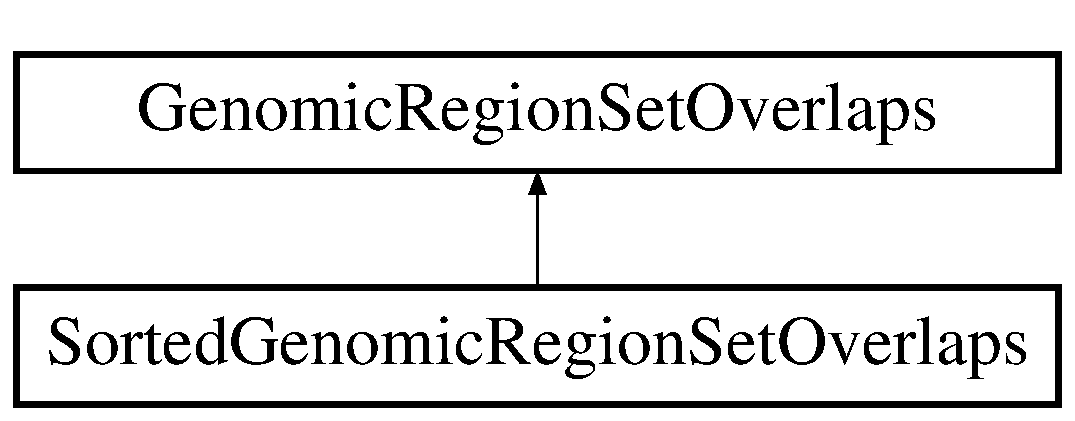
\includegraphics[height=2cm]{classSortedGenomicRegionSetOverlaps}
\end{center}
\end{figure}
\subsection*{Public Member Functions}
\begin{CompactItemize}
\item 
\hyperlink{classSortedGenomicRegionSetOverlaps_0213f6ea908db759f63cea80db4909aa}{SortedGenomicRegionSetOverlaps} (\hyperlink{classGenomicRegionSet}{GenomicRegionSet} $\ast$\hyperlink{classGenomicRegionSetOverlaps_e513304379055f6d379bc5907733dbe2}{QuerySet}, \hyperlink{classGenomicRegionSet}{GenomicRegionSet} $\ast$\hyperlink{classGenomicRegionSetOverlaps_c587bf854c827381493735b473622e03}{IndexSet}, bool \hyperlink{classSortedGenomicRegionSetOverlaps_f08c449faa6ba7be7c6ed9c07f4226e3}{sorted\_\-by\_\-strand})
\begin{CompactList}\small\item\em Class constructor. \item\end{CompactList}\item 
\hypertarget{classSortedGenomicRegionSetOverlaps_1ac0a70899fce3684da0b7e915a13d1e}{
\hyperlink{classSortedGenomicRegionSetOverlaps_1ac0a70899fce3684da0b7e915a13d1e}{$\sim$SortedGenomicRegionSetOverlaps} ()}
\label{classSortedGenomicRegionSetOverlaps_1ac0a70899fce3684da0b7e915a13d1e}

\begin{CompactList}\small\item\em Class destructor. \item\end{CompactList}\item 
\hypertarget{classSortedGenomicRegionSetOverlaps_3b187db0a12f876a9347b4a1641670a0}{
\hyperlink{classGenomicRegion}{GenomicRegion} $\ast$ \hyperlink{classSortedGenomicRegionSetOverlaps_3b187db0a12f876a9347b4a1641670a0}{GetQuery} ()}
\label{classSortedGenomicRegionSetOverlaps_3b187db0a12f876a9347b4a1641670a0}

\begin{CompactList}\small\item\em Returns a pointer to the current query region ('NULL' if no more query regions are available); also, \hyperlink{classSortedGenomicRegionSetOverlaps_19fa18e6abd9f045786698fff48a445f}{SortedGenomicRegionSetOverlaps::IRegBuffer} is automatically updated via \hyperlink{classSortedGenomicRegionSetOverlaps_d894d118c61c3cd11be8b37b8f185120}{SortedGenomicRegionSetOverlaps::LoadIndexBuffer}. \item\end{CompactList}\item 
\hypertarget{classSortedGenomicRegionSetOverlaps_127edf3e9d8fb2ebf189af00e6893e96}{
\hyperlink{classGenomicRegion}{GenomicRegion} $\ast$ \hyperlink{classSortedGenomicRegionSetOverlaps_127edf3e9d8fb2ebf189af00e6893e96}{NextQuery} ()}
\label{classSortedGenomicRegionSetOverlaps_127edf3e9d8fb2ebf189af00e6893e96}

\begin{CompactList}\small\item\em Returns a pointer to the next query region ('NULL' if no more query regions are available); also, \hyperlink{classSortedGenomicRegionSetOverlaps_19fa18e6abd9f045786698fff48a445f}{SortedGenomicRegionSetOverlaps::IRegBuffer} is automatically updated via \hyperlink{classSortedGenomicRegionSetOverlaps_d894d118c61c3cd11be8b37b8f185120}{SortedGenomicRegionSetOverlaps::LoadIndexBuffer}. \item\end{CompactList}\item 
\hypertarget{classSortedGenomicRegionSetOverlaps_d0f7b48e1eb685f0aa62aa799088dbc7}{
\hyperlink{classGenomicRegion}{GenomicRegion} $\ast$ \hyperlink{classSortedGenomicRegionSetOverlaps_d0f7b48e1eb685f0aa62aa799088dbc7}{GetMatch} ()}
\label{classSortedGenomicRegionSetOverlaps_d0f7b48e1eb685f0aa62aa799088dbc7}

\begin{CompactList}\small\item\em Returns a pointer to the current index region that overlaps the current query region (even if the overlap is only in the gaps between intervals). \item\end{CompactList}\item 
\hypertarget{classSortedGenomicRegionSetOverlaps_756bad7ba9a862ae27cd9ad52acbeef2}{
\hyperlink{classGenomicRegion}{GenomicRegion} $\ast$ \hyperlink{classSortedGenomicRegionSetOverlaps_756bad7ba9a862ae27cd9ad52acbeef2}{NextMatch} ()}
\label{classSortedGenomicRegionSetOverlaps_756bad7ba9a862ae27cd9ad52acbeef2}

\begin{CompactList}\small\item\em Returns a pointer to the next index region that overlaps the current query region (even if the overlap is only in the gaps between intervals). \item\end{CompactList}\item 
\hypertarget{classSortedGenomicRegionSetOverlaps_726105d1ee63db6271a90e8092e243c9}{
bool \hyperlink{classSortedGenomicRegionSetOverlaps_726105d1ee63db6271a90e8092e243c9}{Done} ()}
\label{classSortedGenomicRegionSetOverlaps_726105d1ee63db6271a90e8092e243c9}

\begin{CompactList}\small\item\em Returns true, if no more query or index regions are available and the \hyperlink{classSortedGenomicRegionSetOverlaps_19fa18e6abd9f045786698fff48a445f}{SortedGenomicRegionSetOverlaps::IRegBuffer} buffer is empty. \item\end{CompactList}\end{CompactItemize}
\subsection*{Private Member Functions}
\begin{CompactItemize}
\item 
\hypertarget{classSortedGenomicRegionSetOverlaps_d894d118c61c3cd11be8b37b8f185120}{
void \hyperlink{classSortedGenomicRegionSetOverlaps_d894d118c61c3cd11be8b37b8f185120}{LoadIndexBuffer} ()}
\label{classSortedGenomicRegionSetOverlaps_d894d118c61c3cd11be8b37b8f185120}

\begin{CompactList}\small\item\em manages \hyperlink{classSortedGenomicRegionSetOverlaps_19fa18e6abd9f045786698fff48a445f}{SortedGenomicRegionSetOverlaps::IRegBuffer} \item\end{CompactList}\item 
\hypertarget{classSortedGenomicRegionSetOverlaps_c5fe4552253a9d9d802d76b0f4356947}{
void \hyperlink{classSortedGenomicRegionSetOverlaps_c5fe4552253a9d9d802d76b0f4356947}{ClearIndexBuffer} ()}
\label{classSortedGenomicRegionSetOverlaps_c5fe4552253a9d9d802d76b0f4356947}

\begin{CompactList}\small\item\em clears \hyperlink{classSortedGenomicRegionSetOverlaps_19fa18e6abd9f045786698fff48a445f}{SortedGenomicRegionSetOverlaps::IRegBuffer} \item\end{CompactList}\end{CompactItemize}
\subsection*{Private Attributes}
\begin{CompactItemize}
\item 
\hypertarget{classSortedGenomicRegionSetOverlaps_f08c449faa6ba7be7c6ed9c07f4226e3}{
bool \hyperlink{classSortedGenomicRegionSetOverlaps_f08c449faa6ba7be7c6ed9c07f4226e3}{sorted\_\-by\_\-strand}}
\label{classSortedGenomicRegionSetOverlaps_f08c449faa6ba7be7c6ed9c07f4226e3}

\begin{CompactList}\small\item\em if true, query and index regions sorted by strand \item\end{CompactList}\item 
\hypertarget{classSortedGenomicRegionSetOverlaps_19fa18e6abd9f045786698fff48a445f}{
GenomicRegionList \hyperlink{classSortedGenomicRegionSetOverlaps_19fa18e6abd9f045786698fff48a445f}{IRegBuffer}}
\label{classSortedGenomicRegionSetOverlaps_19fa18e6abd9f045786698fff48a445f}

\begin{CompactList}\small\item\em temporary buffer containing index regions that overlap with current query; the buffer is cleared only if the next query has no overlap \item\end{CompactList}\item 
\hypertarget{classSortedGenomicRegionSetOverlaps_71d6eea0c4bf9f19be6cf0c0c562f297}{
GenomicRegionList::iterator \hyperlink{classSortedGenomicRegionSetOverlaps_71d6eea0c4bf9f19be6cf0c0c562f297}{IRegBufferIterator}}
\label{classSortedGenomicRegionSetOverlaps_71d6eea0c4bf9f19be6cf0c0c562f297}

\begin{CompactList}\small\item\em iterator on \hyperlink{classSortedGenomicRegionSetOverlaps_19fa18e6abd9f045786698fff48a445f}{SortedGenomicRegionSetOverlaps::IRegBuffer} \item\end{CompactList}\item 
\hypertarget{classSortedGenomicRegionSetOverlaps_962f8e6ce8c15703cfefa574a07ce42c}{
\hyperlink{classGenomicInterval}{GenomicInterval} $\ast$ \hyperlink{classSortedGenomicRegionSetOverlaps_962f8e6ce8c15703cfefa574a07ce42c}{ireg\_\-buffer\_\-interval}}
\label{classSortedGenomicRegionSetOverlaps_962f8e6ce8c15703cfefa574a07ce42c}

\begin{CompactList}\small\item\em keeps tracks of the (linked) interval stored in \hyperlink{classSortedGenomicRegionSetOverlaps_19fa18e6abd9f045786698fff48a445f}{SortedGenomicRegionSetOverlaps::IRegBuffer} \item\end{CompactList}\item 
\hypertarget{classSortedGenomicRegionSetOverlaps_349d589ff006f742d635b16987fe7b6b}{
unsigned long int \hyperlink{classSortedGenomicRegionSetOverlaps_349d589ff006f742d635b16987fe7b6b}{max\_\-ireg\_\-buffer\_\-size}}
\label{classSortedGenomicRegionSetOverlaps_349d589ff006f742d635b16987fe7b6b}

\begin{CompactList}\small\item\em keeps track of the maximum size of \hyperlink{classSortedGenomicRegionSetOverlaps_19fa18e6abd9f045786698fff48a445f}{SortedGenomicRegionSetOverlaps::IRegBuffer} \item\end{CompactList}\end{CompactItemize}


\subsection{Detailed Description}
This class is used to find overlaps between two genomic regions sets. See detailed description below for an example. 

A simple example for computing RNAseq read densities in known exons (this is actually implemented in the {\bf genomic\_\-overlaps} command-line tool as 'density' operation): 

\begin{Code}\begin{verbatim}    // open region sets
    char *QUERY_REG_FILE = "rnaseq.reads.reg";
    char *INDEX_REG_FILE = "exons.reg";
    double MIN_DENSITY = 0.0;
    bool SORTED_BY_STRAND = false; 
    GenomicRegionSet QueryRegSet(QUERY_REG_FILE,10000,true,false);
    GenomicRegionSet IndexRegSet(INDEX_REG_FILE,10000,true,false);

    SortedGenomicRegionSetOverlaps Overlaps(&QueryRegSet,&IndexRegSet,SORTED_BY_STRAND);
    Progress PRG("Processing queries...",1);
    for (GenomicRegion *qreg=Overlaps.GetQuery(); qreg!=NULL; qreg=Overlaps.NextQuery()) {
      double density = (double)Overlaps.CalcCoverage(USE_VALUES,IGNORE_STRAND)/qreg->GetSize(); 
      if (density>=MIN_DENSITY) printf("%s\t%.4e\n", qreg->LABEL, density);
      PRG.Check();
    }
    PRG.Done();
\end{verbatim}
\end{Code}

 A more complex example for creating ChIPseq read profiles in TSS regions (this is actually implemented in the {\bf genomic\_\-overlaps} command-line tool as 'offset' operation): 

\begin{Code}\begin{verbatim}    // open region sets
    char *QUERY_REG_FILE = "chipseq.reads.reg";
    char *INDEX_REG_FILE = "TSS.flank10kb.reg";
    char *OFFSET_OP = "5p";
    bool SORTED_BY_STRAND = false; 
    bool MATCH_GAPS = true;
    bool IGNORE_STRAND = true;
    GenomicRegionSet QueryRegSet(QUERY_REG_FILE,10000,true,false);
    GenomicRegionSet IndexRegSet(INDEX_REG_FILE,10000,true,false);

    SortedGenomicRegionSetOverlaps Overlaps(&QueryRegSet,&IndexRegSet,SORTED_BY_STRAND);
    Progress PRG("Processing queries...",1);
    for (GenomicRegion *qreg=Overlaps.GetQuery(); Overlaps.Done()==false; qreg=Overlaps.NextQuery()) {
      size_t Qsize = qreg->GetSize();
      for (GenomicRegion *ireg=Overlaps.GetOverlap(MATCH_GAPS,IGNORE_STRAND); ireg!=NULL; ireg=Overlaps.NextOverlap(MATCH_GAPS,IGNORE_STRAND)) {
        cout << qreg->LABEL << '\t';
        long int start_offset, stop_offset;
        ireg->I.front()->GetOffsetFrom(qreg->I.front(),OFFSET_OP,IGNORE_STRAND,&start_offset,&stop_offset);
        printf("%f", ((float)start_offset/Qsize+(float)stop_offset/Qsize)/2); 
        cout << '\n';
      }
      PRG.Check();
    }
    PRG.Done();
\end{verbatim}
\end{Code}

 

\subsection{Constructor \& Destructor Documentation}
\hypertarget{classSortedGenomicRegionSetOverlaps_0213f6ea908db759f63cea80db4909aa}{
\index{SortedGenomicRegionSetOverlaps@{SortedGenomicRegionSetOverlaps}!SortedGenomicRegionSetOverlaps@{SortedGenomicRegionSetOverlaps}}
\index{SortedGenomicRegionSetOverlaps@{SortedGenomicRegionSetOverlaps}!SortedGenomicRegionSetOverlaps@{SortedGenomicRegionSetOverlaps}}
\subsubsection[SortedGenomicRegionSetOverlaps]{\setlength{\rightskip}{0pt plus 5cm}SortedGenomicRegionSetOverlaps::SortedGenomicRegionSetOverlaps ({\bf GenomicRegionSet} $\ast$ {\em QuerySet}, \/  {\bf GenomicRegionSet} $\ast$ {\em IndexSet}, \/  bool {\em sorted\_\-by\_\-strand})}}
\label{classSortedGenomicRegionSetOverlaps_0213f6ea908db759f63cea80db4909aa}


Class constructor. 

\begin{Desc}
\item[Parameters:]
\begin{description}
\item[{\em QuerySet}]pointer to query region set \item[{\em IndexSet}]pointer to index region set \item[{\em sorted\_\-by\_\-strand}]if true, query and index regions are sorted by strand \end{description}
\end{Desc}


The documentation for this class was generated from the following files:\begin{CompactItemize}
\item 
genomic\_\-intervals.h\item 
genomic\_\-intervals.cpp\end{CompactItemize}

\hypertarget{classUnsortedGenomicRegionSetOverlaps}{
\section{UnsortedGenomicRegionSetOverlaps Class Reference}
\label{classUnsortedGenomicRegionSetOverlaps}\index{UnsortedGenomicRegionSetOverlaps@{UnsortedGenomicRegionSetOverlaps}}
}
\mbox{[}UNDER DEVELOPMENT\mbox{]} Class for computing overlaps between unsorted regions.  


{\tt \#include $<$genomic\_\-intervals.h$>$}

Inheritance diagram for UnsortedGenomicRegionSetOverlaps::\begin{figure}[H]
\begin{center}
\leavevmode
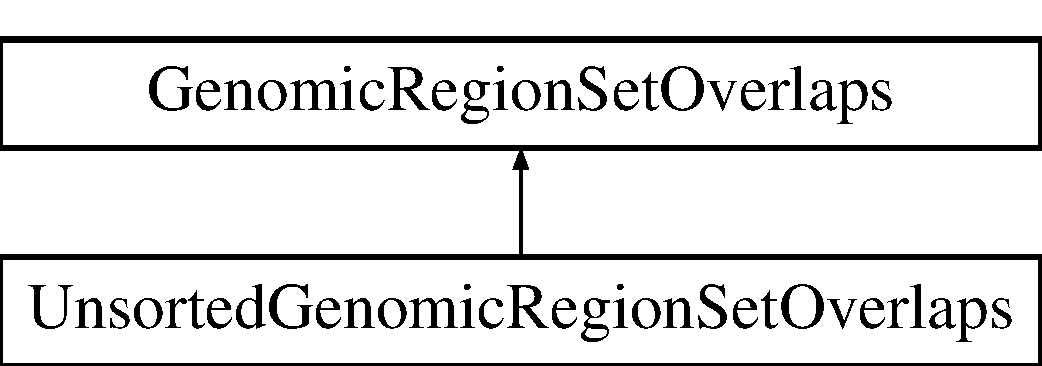
\includegraphics[height=2cm]{classUnsortedGenomicRegionSetOverlaps}
\end{center}
\end{figure}
\subsection*{Public Types}
\begin{CompactItemize}
\item 
\hypertarget{classUnsortedGenomicRegionSetOverlaps_0f0857dd93ad3c047d1f5056a57edc14}{
typedef pair$<$ long int $\ast$, long int $\ast$$\ast$ $>$ \hyperlink{classUnsortedGenomicRegionSetOverlaps_0f0857dd93ad3c047d1f5056a57edc14}{BinSet}}
\label{classUnsortedGenomicRegionSetOverlaps_0f0857dd93ad3c047d1f5056a57edc14}

\begin{CompactList}\small\item\em a two-dimensional grid of bins \item\end{CompactList}\end{CompactItemize}
\subsection*{Public Member Functions}
\begin{CompactItemize}
\item 
\hyperlink{classUnsortedGenomicRegionSetOverlaps_6a1255dfaac34080fae7880981b47acb}{UnsortedGenomicRegionSetOverlaps} (\hyperlink{classGenomicRegionSet}{GenomicRegionSet} $\ast$\hyperlink{classGenomicRegionSetOverlaps_e513304379055f6d379bc5907733dbe2}{QuerySet}, \hyperlink{classGenomicRegionSet}{GenomicRegionSet} $\ast$\hyperlink{classGenomicRegionSetOverlaps_c587bf854c827381493735b473622e03}{IndexSet})
\begin{CompactList}\small\item\em Class constructor. \item\end{CompactList}\item 
\hypertarget{classUnsortedGenomicRegionSetOverlaps_7682171bb52c651af44e4e8f3bf33f52}{
\hyperlink{classUnsortedGenomicRegionSetOverlaps_7682171bb52c651af44e4e8f3bf33f52}{$\sim$UnsortedGenomicRegionSetOverlaps} ()}
\label{classUnsortedGenomicRegionSetOverlaps_7682171bb52c651af44e4e8f3bf33f52}

\begin{CompactList}\small\item\em Class destructor. \item\end{CompactList}\item 
\hypertarget{classUnsortedGenomicRegionSetOverlaps_bf7e2f8d35f7a9cf8441caa9d765de44}{
\hyperlink{classGenomicRegion}{GenomicRegion} $\ast$ \hyperlink{classUnsortedGenomicRegionSetOverlaps_bf7e2f8d35f7a9cf8441caa9d765de44}{GetQuery} ()}
\label{classUnsortedGenomicRegionSetOverlaps_bf7e2f8d35f7a9cf8441caa9d765de44}

\begin{CompactList}\small\item\em Returns a pointer to the current query region ('NULL' if no more query regions are available). \item\end{CompactList}\item 
\hypertarget{classUnsortedGenomicRegionSetOverlaps_96e68ef99a958665f5da74572edcc854}{
\hyperlink{classGenomicRegion}{GenomicRegion} $\ast$ \hyperlink{classUnsortedGenomicRegionSetOverlaps_96e68ef99a958665f5da74572edcc854}{NextQuery} ()}
\label{classUnsortedGenomicRegionSetOverlaps_96e68ef99a958665f5da74572edcc854}

\begin{CompactList}\small\item\em Returns a pointer to the next query region ('NULL' if no more query regions are available). \item\end{CompactList}\item 
\hypertarget{classUnsortedGenomicRegionSetOverlaps_61c2c6e9203acb0e0a9bfa4f0176308f}{
\hyperlink{classGenomicRegion}{GenomicRegion} $\ast$ \hyperlink{classUnsortedGenomicRegionSetOverlaps_61c2c6e9203acb0e0a9bfa4f0176308f}{GetMatch} ()}
\label{classUnsortedGenomicRegionSetOverlaps_61c2c6e9203acb0e0a9bfa4f0176308f}

\begin{CompactList}\small\item\em Returns a pointer to the current index region that overlaps the current query region (even if the overlap is only in the gaps between intervals). \item\end{CompactList}\item 
\hypertarget{classUnsortedGenomicRegionSetOverlaps_0bcd12697611caa5216db7a4c4fca4e2}{
\hyperlink{classGenomicRegion}{GenomicRegion} $\ast$ \hyperlink{classUnsortedGenomicRegionSetOverlaps_0bcd12697611caa5216db7a4c4fca4e2}{NextMatch} ()}
\label{classUnsortedGenomicRegionSetOverlaps_0bcd12697611caa5216db7a4c4fca4e2}

\begin{CompactList}\small\item\em Returns a pointer to the next index region that overlaps the current query region (even if the overlap is only in the gaps between intervals). \item\end{CompactList}\item 
\hypertarget{classUnsortedGenomicRegionSetOverlaps_fc18fc203debad6a2d48200ea8ccb42f}{
bool \hyperlink{classUnsortedGenomicRegionSetOverlaps_fc18fc203debad6a2d48200ea8ccb42f}{Done} ()}
\label{classUnsortedGenomicRegionSetOverlaps_fc18fc203debad6a2d48200ea8ccb42f}

\begin{CompactList}\small\item\em Returns true, if no more query or index regions are available and the \hyperlink{classSortedGenomicRegionSetOverlaps_19fa18e6abd9f045786698fff48a445f}{SortedGenomicRegionSetOverlaps::IRegBuffer} buffer is empty. \item\end{CompactList}\end{CompactItemize}
\subsection*{Public Attributes}
\begin{CompactItemize}
\item 
\hypertarget{classUnsortedGenomicRegionSetOverlaps_251e09b7f0a13a56b902c30791228ce4}{
long int $\ast$ \hyperlink{classUnsortedGenomicRegionSetOverlaps_251e09b7f0a13a56b902c30791228ce4}{r\_\-next}}
\label{classUnsortedGenomicRegionSetOverlaps_251e09b7f0a13a56b902c30791228ce4}

\begin{CompactList}\small\item\em for each region store, store a pointer to the \char`\"{}next\char`\"{} one in the same bin \item\end{CompactList}\item 
\hypertarget{classUnsortedGenomicRegionSetOverlaps_1cc721de471ed40dcc7d8eae258e5833}{
int \hyperlink{classUnsortedGenomicRegionSetOverlaps_1cc721de471ed40dcc7d8eae258e5833}{n\_\-levels}}
\label{classUnsortedGenomicRegionSetOverlaps_1cc721de471ed40dcc7d8eae258e5833}

\begin{CompactList}\small\item\em number of levels in the two-dimensional grid of bins \item\end{CompactList}\item 
\hypertarget{classUnsortedGenomicRegionSetOverlaps_76ecebfcf839a940bdae26069ceef748}{
int $\ast$ \hyperlink{classUnsortedGenomicRegionSetOverlaps_76ecebfcf839a940bdae26069ceef748}{n\_\-bits}}
\label{classUnsortedGenomicRegionSetOverlaps_76ecebfcf839a940bdae26069ceef748}

\begin{CompactList}\small\item\em number of bits (per level) by which the start position is right-shifted to compute its bin \item\end{CompactList}\item 
\hypertarget{classUnsortedGenomicRegionSetOverlaps_beeb94562abdf4aebc36684959a5bc78}{
map$<$ string, \hyperlink{classUnsortedGenomicRegionSetOverlaps_0f0857dd93ad3c047d1f5056a57edc14}{BinSet} $\ast$ $>$ \hyperlink{classUnsortedGenomicRegionSetOverlaps_beeb94562abdf4aebc36684959a5bc78}{index}}
\label{classUnsortedGenomicRegionSetOverlaps_beeb94562abdf4aebc36684959a5bc78}

\begin{CompactList}\small\item\em the two-dimensional grid of bins per chromosome \item\end{CompactList}\item 
\hypertarget{classUnsortedGenomicRegionSetOverlaps_6bbb87f3c66d04527f06a5761df1ab56}{
\hyperlink{classUnsortedGenomicRegionSetOverlaps_0f0857dd93ad3c047d1f5056a57edc14}{BinSet} $\ast$ \hyperlink{classUnsortedGenomicRegionSetOverlaps_6bbb87f3c66d04527f06a5761df1ab56}{current\_\-binset}}
\label{classUnsortedGenomicRegionSetOverlaps_6bbb87f3c66d04527f06a5761df1ab56}

\begin{CompactList}\small\item\em pointer to the current chromosome set of bins \item\end{CompactList}\item 
\hypertarget{classUnsortedGenomicRegionSetOverlaps_bafc544ce2c677ce071fa4e30ec2ecaf}{
bool \hyperlink{classUnsortedGenomicRegionSetOverlaps_bafc544ce2c677ce071fa4e30ec2ecaf}{new\_\-query}}
\label{classUnsortedGenomicRegionSetOverlaps_bafc544ce2c677ce071fa4e30ec2ecaf}

\begin{CompactList}\small\item\em 'true', if a new query is about to be processed \item\end{CompactList}\end{CompactItemize}


\subsection{Detailed Description}
\mbox{[}UNDER DEVELOPMENT\mbox{]} Class for computing overlaps between unsorted regions. 

\subsection{Constructor \& Destructor Documentation}
\hypertarget{classUnsortedGenomicRegionSetOverlaps_6a1255dfaac34080fae7880981b47acb}{
\index{UnsortedGenomicRegionSetOverlaps@{UnsortedGenomicRegionSetOverlaps}!UnsortedGenomicRegionSetOverlaps@{UnsortedGenomicRegionSetOverlaps}}
\index{UnsortedGenomicRegionSetOverlaps@{UnsortedGenomicRegionSetOverlaps}!UnsortedGenomicRegionSetOverlaps@{UnsortedGenomicRegionSetOverlaps}}
\subsubsection[UnsortedGenomicRegionSetOverlaps]{\setlength{\rightskip}{0pt plus 5cm}UnsortedGenomicRegionSetOverlaps::UnsortedGenomicRegionSetOverlaps ({\bf GenomicRegionSet} $\ast$ {\em QuerySet}, \/  {\bf GenomicRegionSet} $\ast$ {\em IndexSet})}}
\label{classUnsortedGenomicRegionSetOverlaps_6a1255dfaac34080fae7880981b47acb}


Class constructor. 

\begin{Desc}
\item[Parameters:]
\begin{description}
\item[{\em QuerySet}]pointer to query region set \item[{\em IndexSet}]pointer to index region set \end{description}
\end{Desc}


The documentation for this class was generated from the following files:\begin{CompactItemize}
\item 
genomic\_\-intervals.h\item 
genomic\_\-intervals.cpp\end{CompactItemize}

\printindex
\end{document}
